\documentclass[12pt]{extarticle}
\usepackage[paperwidth=15in,paperheight=7.2in]{geometry}
\usepackage{amsmath}
\usepackage{hyperref}
\usepackage{multirow}
\usepackage{pdfpages}
\usepackage[utf8]{inputenc}
\title{Kaon mixing: chiral and continuum extrapolations}
\author{R Mukherjee}
\date{\today}
\begin{document}
\maketitle
\tableofcontents
\clearpage
\begin{figure}
\centering
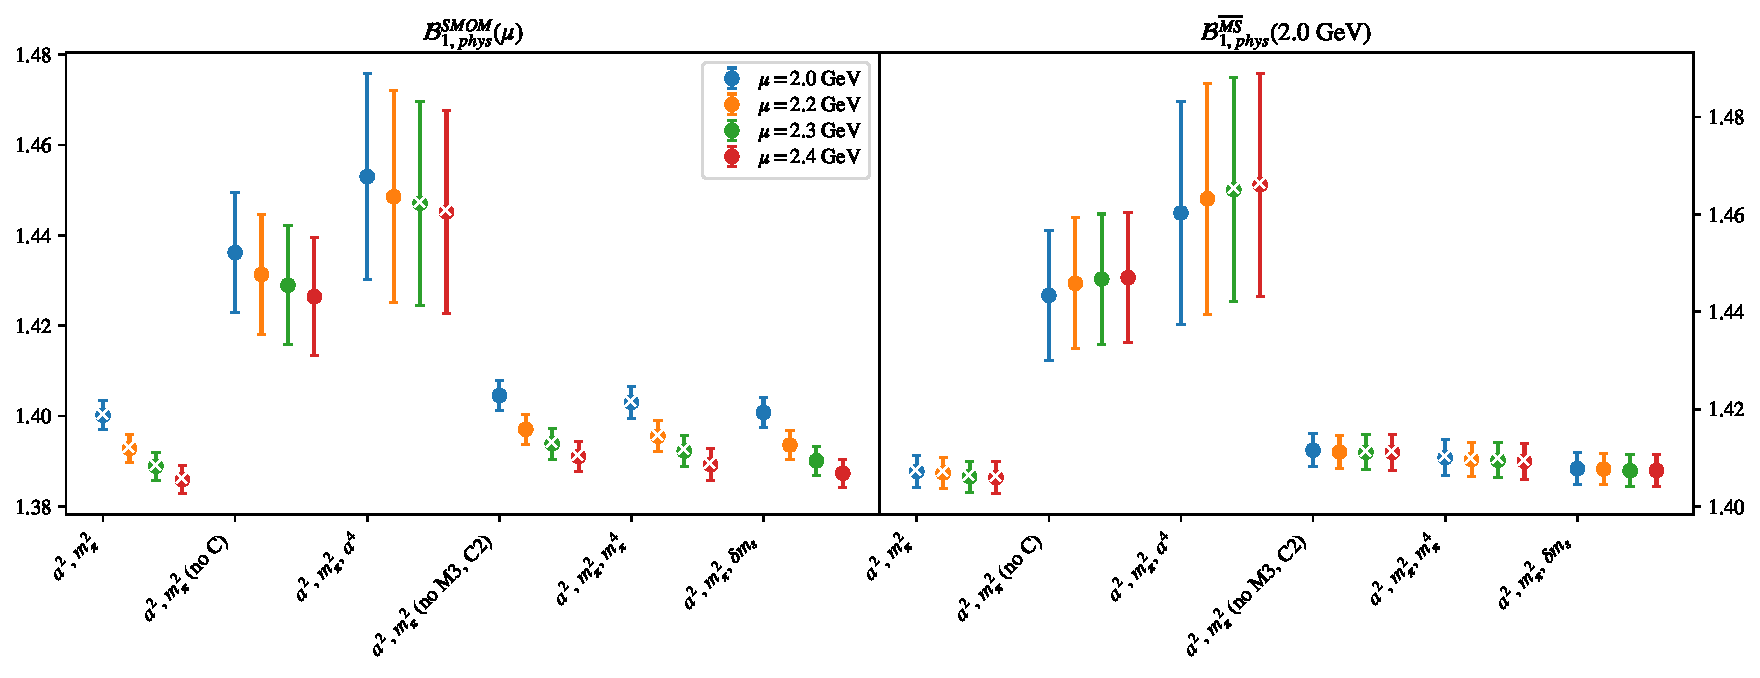
\includegraphics[page=1, width=1.1\textwidth]{VVpAA/NPR/fit_summary_bag.pdf}
\caption{$\mathcal{B}_{1}$\\(left) $\mathcal{B}_{phys}$ in RI/SMOM scheme from fit variations (fits with $p$-value $<0.05$ marked with ``$\times$"). \\(right) $\mathcal{B}_{phys}$ in $\overline{MS}$ computed using $\mathcal{B}^{\overline{MS}} = R^{\overline{MS}\leftarrow SMOM}(2.0)\sigma_{npt}(2.0,\mu) \mathcal{B}^{SMOM}(\mu)$.}
\end{figure}
\clearpage
\begin{figure}
\centering
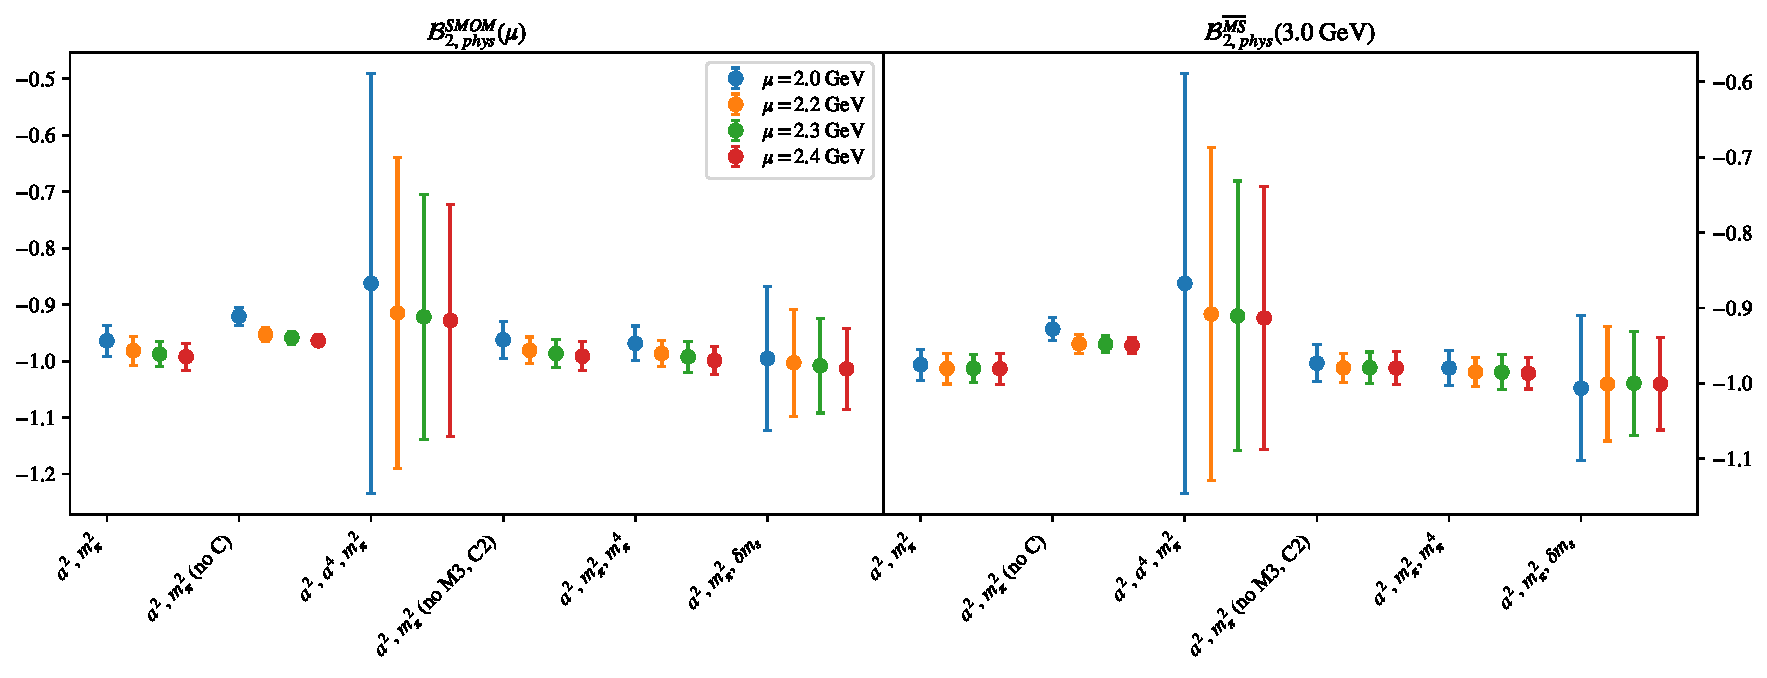
\includegraphics[page=1, width=1.1\textwidth]{VVmAA/NPR/fit_summary_bag.pdf}
\caption{$\mathcal{B}_{2}$\\(left) $\mathcal{B}_{phys}$ in RI/SMOM scheme from fit variations (fits with $p$-value $<0.05$ marked with ``$\times$"). \\(right) $\mathcal{B}_{phys}$ in $\overline{MS}$ computed using $\mathcal{B}^{\overline{MS}} = R^{\overline{MS}\leftarrow SMOM}(3.0)\sigma_{npt}(3.0,\mu) \mathcal{B}^{SMOM}(\mu)$.}
\end{figure}
\clearpage
\begin{figure}
\centering
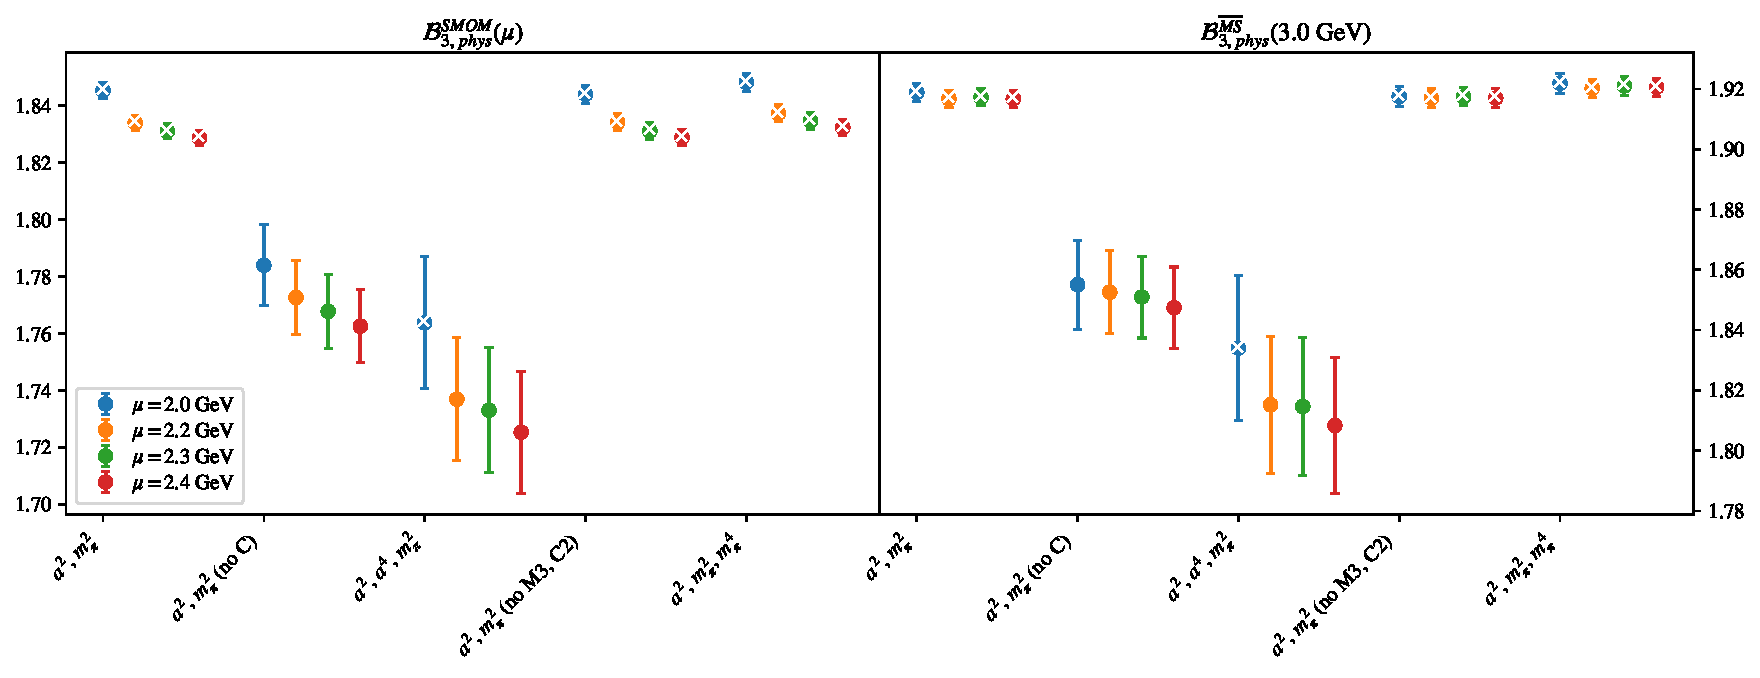
\includegraphics[page=1, width=1.1\textwidth]{SSmPP/NPR/fit_summary_bag.pdf}
\caption{$\mathcal{B}_{3}$\\(left) $\mathcal{B}_{phys}$ in RI/SMOM scheme from fit variations (fits with $p$-value $<0.05$ marked with ``$\times$"). \\(right) $\mathcal{B}_{phys}$ in $\overline{MS}$ computed using $\mathcal{B}^{\overline{MS}} = R^{\overline{MS}\leftarrow SMOM}(3.0)\sigma_{npt}(3.0,\mu) \mathcal{B}^{SMOM}(\mu)$.}
\end{figure}
\clearpage
\begin{figure}
\centering
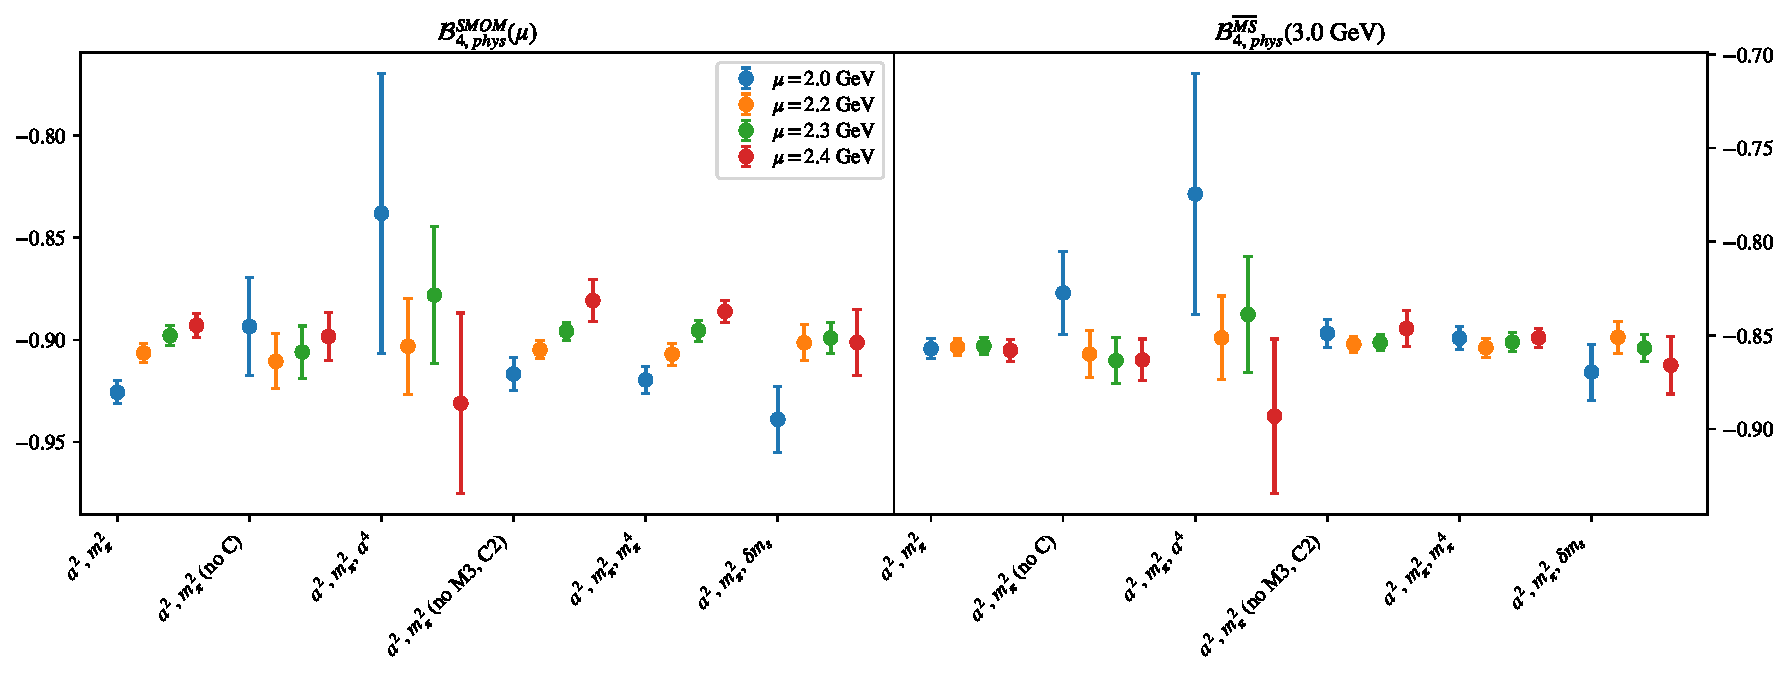
\includegraphics[page=1, width=1.1\textwidth]{SSpPP/NPR/fit_summary_bag.pdf}
\caption{$\mathcal{B}_{4}$\\(left) $\mathcal{B}_{phys}$ in RI/SMOM scheme from fit variations (fits with $p$-value $<0.05$ marked with ``$\times$"). \\(right) $\mathcal{B}_{phys}$ in $\overline{MS}$ computed using $\mathcal{B}^{\overline{MS}} = R^{\overline{MS}\leftarrow SMOM}(3.0)\sigma_{npt}(3.0,\mu) \mathcal{B}^{SMOM}(\mu)$.}
\end{figure}
\clearpage
\begin{figure}
\centering
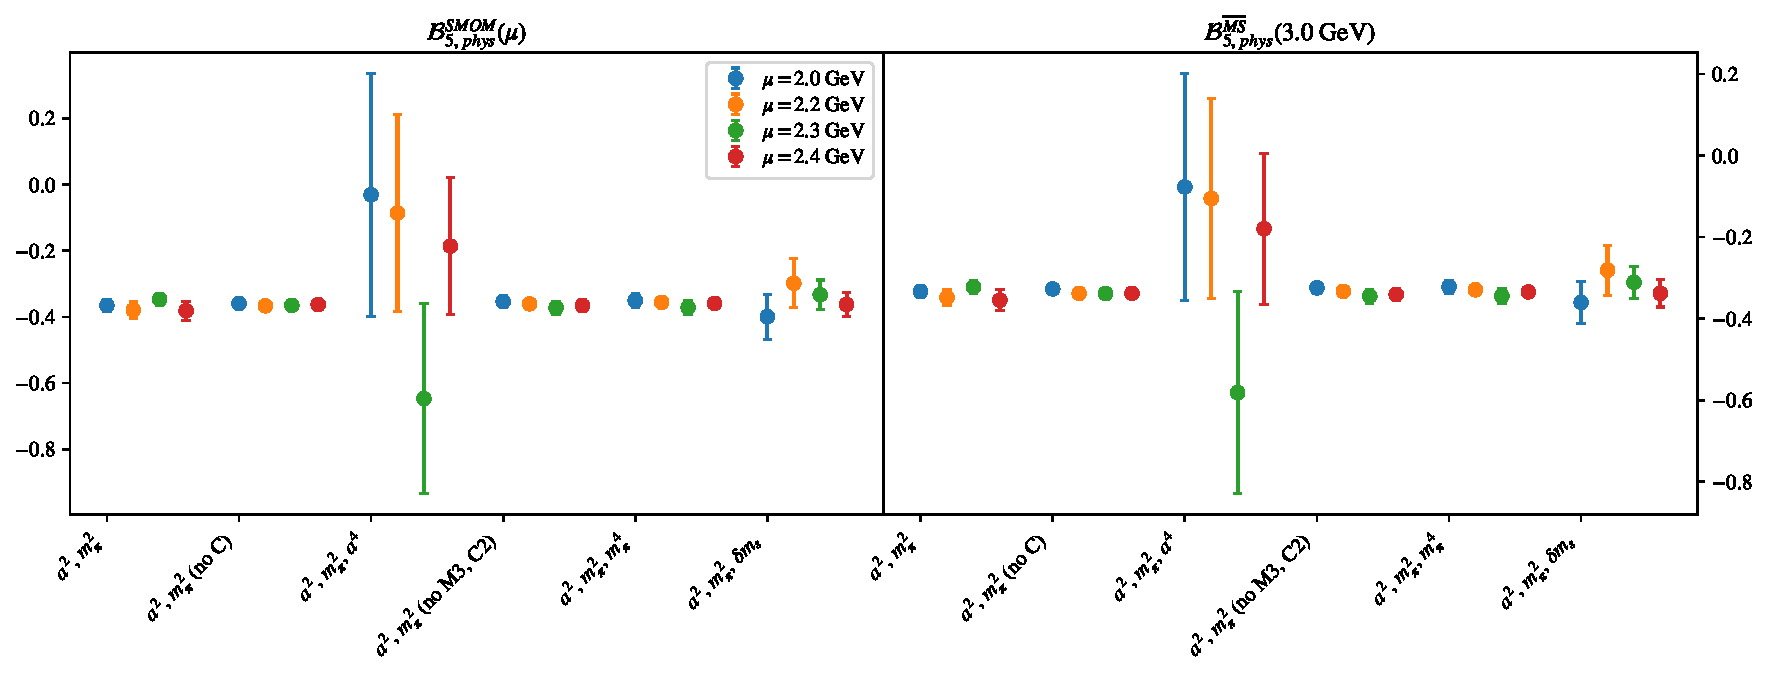
\includegraphics[page=1, width=1.1\textwidth]{TT/NPR/fit_summary_bag.pdf}
\caption{$\mathcal{B}_{5}$\\(left) $\mathcal{B}_{phys}$ in RI/SMOM scheme from fit variations (fits with $p$-value $<0.05$ marked with ``$\times$"). \\(right) $\mathcal{B}_{phys}$ in $\overline{MS}$ computed using $\mathcal{B}^{\overline{MS}} = R^{\overline{MS}\leftarrow SMOM}(3.0)\sigma_{npt}(3.0,\mu) \mathcal{B}^{SMOM}(\mu)$.}
\end{figure}
\clearpage
\section{$\mathcal{B}_1$}
\begin{table}[h!]
\begin{center}
\begin{tabular}{|c|c|c|c|c|c|}
\hline
$\mu$ (GeV) & $a^2$, $m_\pi^2$& $a^2$, $m_\pi^2$ (no C)& $a^2$, $a^4$, $m_\pi^2$& $a^2$, $m_\pi^2$ (no M3, C2)& $a^2$, $m_\pi^2$, $m_\pi^4$\\
\hline
2.0& \hyperlink{VVpAA/NPR/a2m2_20.pdf.1}{\textbf{1.4039(27)}: 1.866 (0.097)} & \hyperlink{VVpAA/NPR/a2m2noC_20.pdf.1}{\textbf{1.416(12)}: 0.927 (0.396)} & \hyperlink{VVpAA/NPR/a2a4m2_20.pdf.1}{\textbf{1.421(21)}: 2.159 (0.071)} & \hyperlink{VVpAA/NPR/a2m2mcut_20.pdf.1}{\textbf{1.4090(32)}: 0.265 (0.851)} & \hyperlink{VVpAA/NPR/a2m2m4_20.pdf.1}{\textbf{1.4092(33)}: 0.698 (0.593)}\\
2.2& \hyperlink{VVpAA/NPR/a2m2_22.pdf.1}{\textbf{1.3964(27)}: 2.198 (0.052)} & \hyperlink{VVpAA/NPR/a2m2noC_22.pdf.1}{\textbf{1.410(12)}: 1.171 (0.31)} & \hyperlink{VVpAA/NPR/a2a4m2_22.pdf.1}{\textbf{1.417(21)}: 2.501 (0.04)} & \hyperlink{VVpAA/NPR/a2m2mcut_22.pdf.1}{\textbf{1.4018(32)}: 0.361 (0.781)} & \hyperlink{VVpAA/NPR/a2m2m4_22.pdf.1}{\textbf{1.4020(33)}: 0.919 (0.452)}\\
2.3& \hyperlink{VVpAA/NPR/a2m2_23.pdf.1}{\textbf{1.3931(27)}: 2.287 (0.043)} & \hyperlink{VVpAA/NPR/a2m2noC_23.pdf.1}{\textbf{1.408(12)}: 1.218 (0.296)} & \hyperlink{VVpAA/NPR/a2a4m2_23.pdf.1}{\textbf{1.415(21)}: 2.579 (0.035)} & \hyperlink{VVpAA/NPR/a2m2mcut_23.pdf.1}{\textbf{1.3986(32)}: 0.411 (0.745)} & \hyperlink{VVpAA/NPR/a2m2m4_23.pdf.1}{\textbf{1.3988(33)}: 0.988 (0.413)}\\
2.4& \hyperlink{VVpAA/NPR/a2m2_24.pdf.1}{\textbf{1.3902(27)}: 2.335 (0.04)} & \hyperlink{VVpAA/NPR/a2m2noC_24.pdf.1}{\textbf{1.405(12)}: 1.243 (0.289)} & \hyperlink{VVpAA/NPR/a2a4m2_24.pdf.1}{\textbf{1.412(21)}: 2.639 (0.032)} & \hyperlink{VVpAA/NPR/a2m2mcut_24.pdf.1}{\textbf{1.3958(32)}: 0.413 (0.744)} & \hyperlink{VVpAA/NPR/a2m2m4_24.pdf.1}{\textbf{1.3960(33)}: 1.004 (0.404)}\\
\hline
\end{tabular}
\caption{Physical point value from chiral and continuum extrapolation at renormalisation scale $\mu$. Entries are \textbf{value(error)}: $\chi^2/\text{DOF}$ ($p$-value).}
\end{center}
\end{table}
\begin{table}[h!]
\begin{center}
\begin{tabular}{|c c|c|c|c|c|c|}
\hline
$\mu$ (GeV) &  & $a^2$, $m_\pi^2$& $a^2$, $m_\pi^2$ (no C)& $a^2$, $a^4$, $m_\pi^2$& $a^2$, $m_\pi^2$ (no M3, C2)& $a^2$, $m_\pi^2$, $m_\pi^4$\\
\hline
\multirow{2}{0.5in}{2.0} & $\alpha$ & 0.0935(72)& 0.047(53)& -0.022& 0.0814(84)& 0.0811(84)\\
 & $\beta$ & 0.00260(15)& 0.00224(27)& 0.00263(15)& 0.00189(28)& 0.00033(88)\\
\hline
\multirow{2}{0.5in}{2.2} & $\alpha$ & 0.0977(72)& 0.042(52)& -0.04& 0.0848(85)& 0.0847(84)\\
 & $\beta$ & 0.00261(15)& 0.00221(27)& 0.00264(15)& 0.00183(28)& 0.00020(88)\\
\hline
\multirow{2}{0.5in}{2.3} & $\alpha$ & 0.0992(72)& 0.039(52)& -0.047& 0.0860(85)& 0.0860(84)\\
 & $\beta$ & 0.00261(15)& 0.00221(27)& 0.00265(15)& 0.00183(28)& 0.00018(88)\\
\hline
\multirow{2}{0.5in}{2.4} & $\alpha$ & 0.0999(72)& 0.040(52)& -0.046& 0.0865(85)& 0.0865(84)\\
 & $\beta$ & 0.00263(15)& 0.00221(27)& 0.00266(15)& 0.00184(28)& 0.00017(88)\\
\hline
\end{tabular}
\caption{Fit values of coefficients in $Q = Q_{phys} + \mathbf{\alpha} a^2 + \mathbf{\beta}\left(\frac{m_\pi^2}{f_\pi^2}-\frac{m_{\pi,PDG}^2}{f_\pi^2}\right) + \ldots$.}
\end{center}
\end{table}
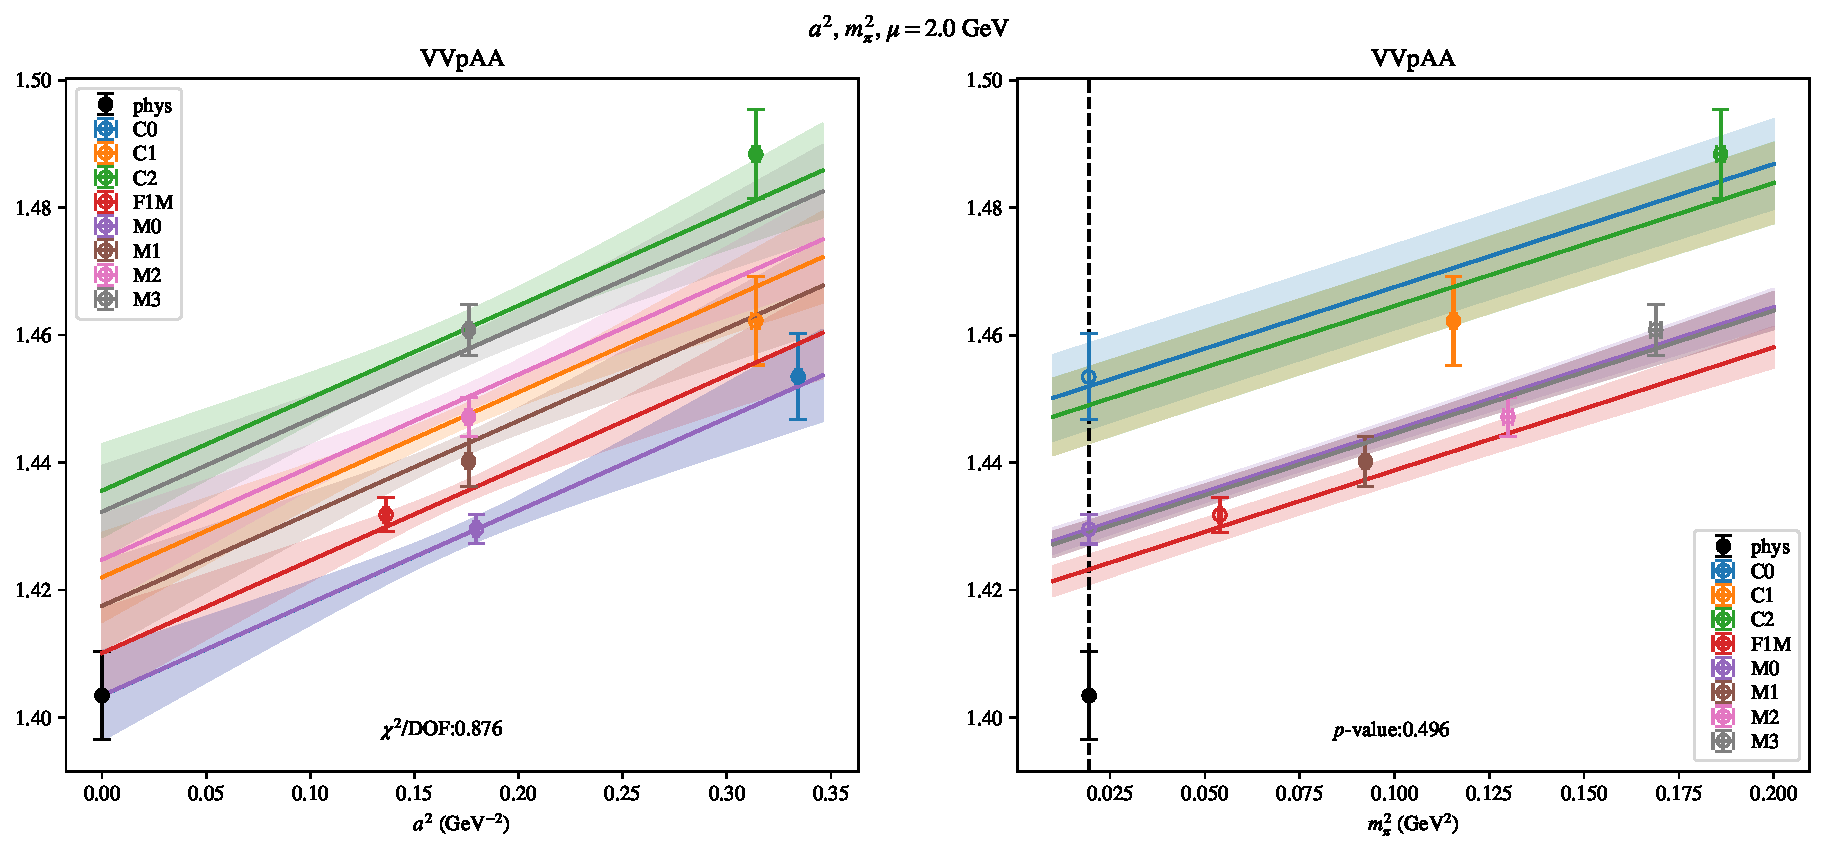
\includepdf[link, pages=-]{VVpAA/NPR/a2m2_20.pdf}
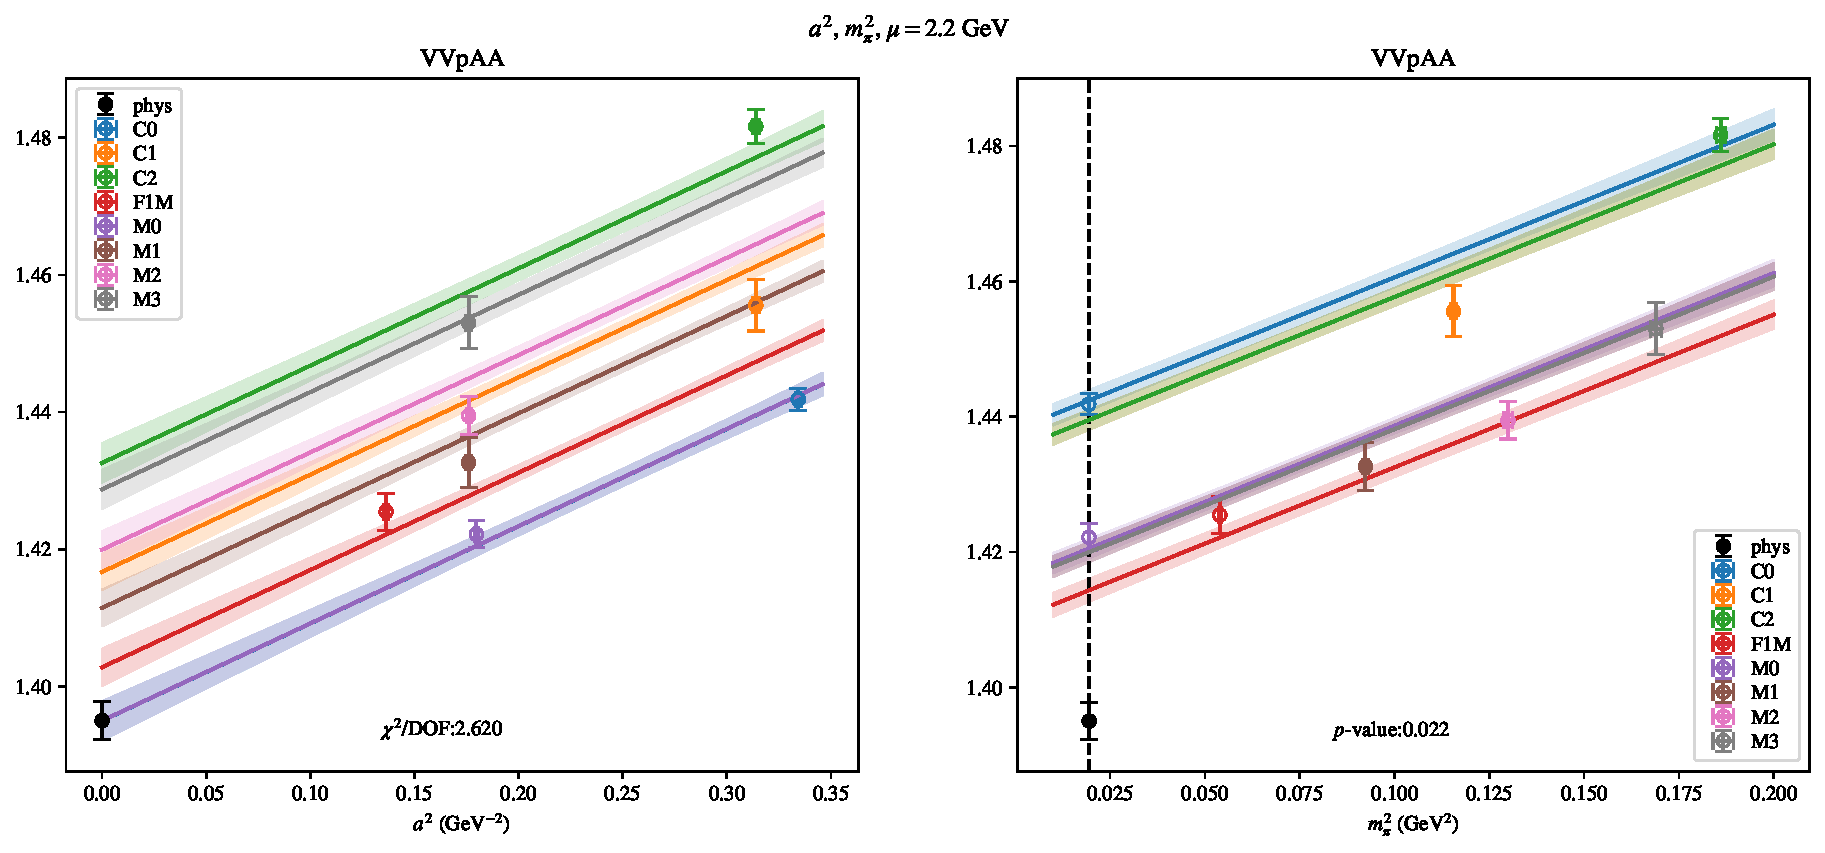
\includepdf[link, pages=-]{VVpAA/NPR/a2m2_22.pdf}
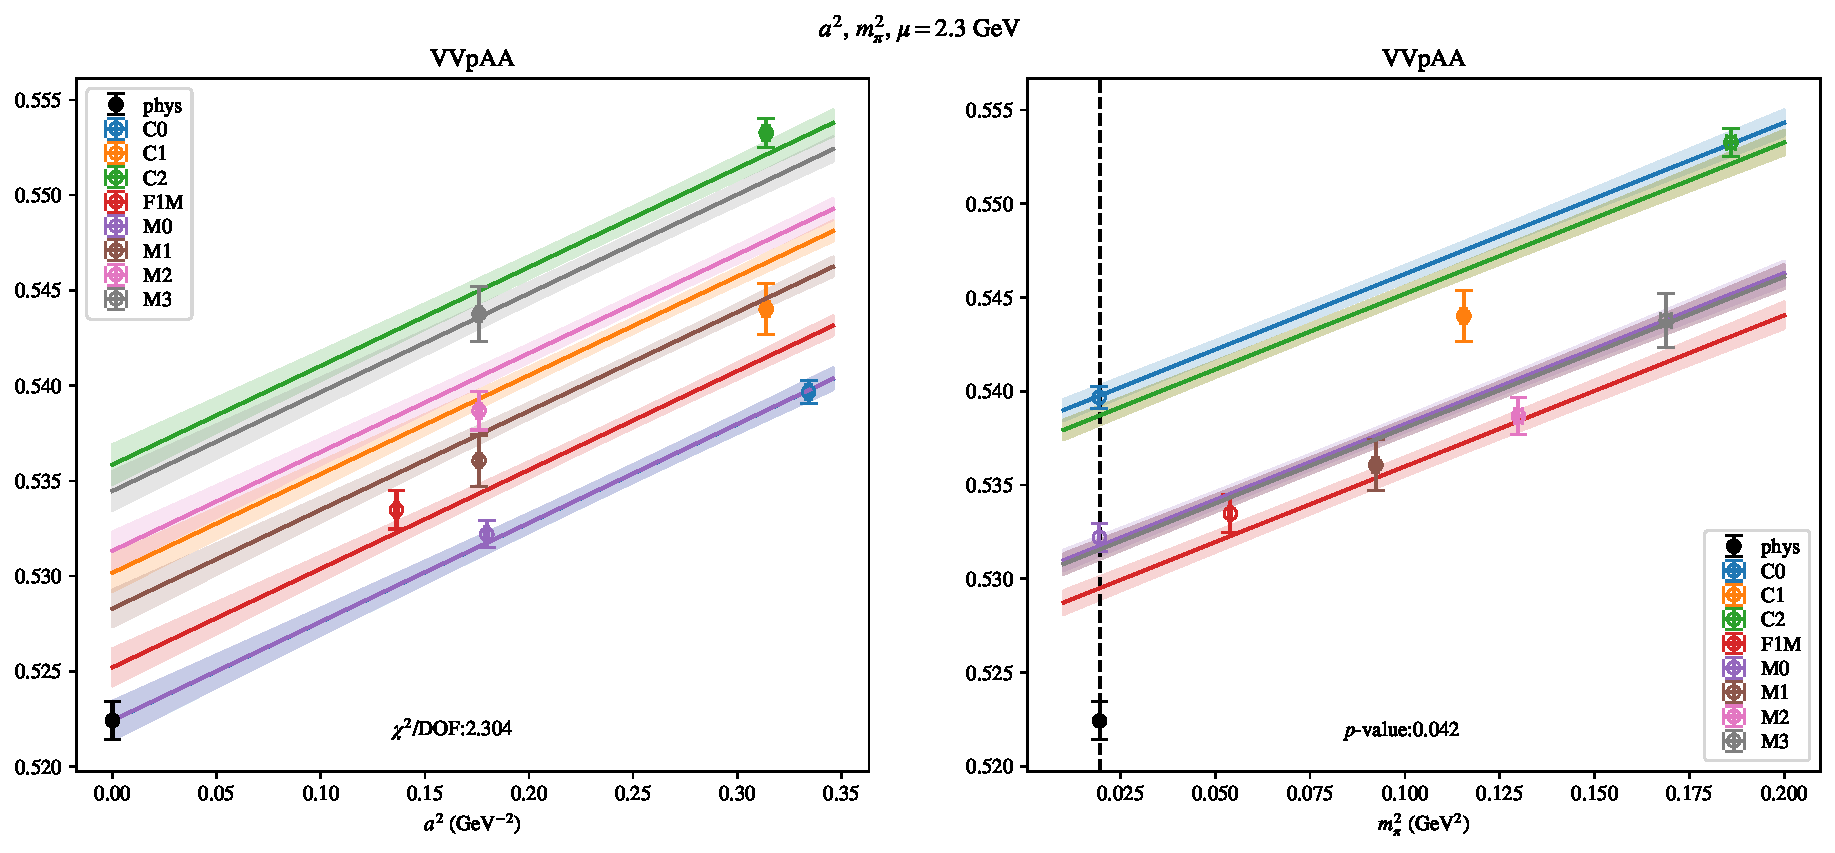
\includepdf[link, pages=-]{VVpAA/NPR/a2m2_23.pdf}
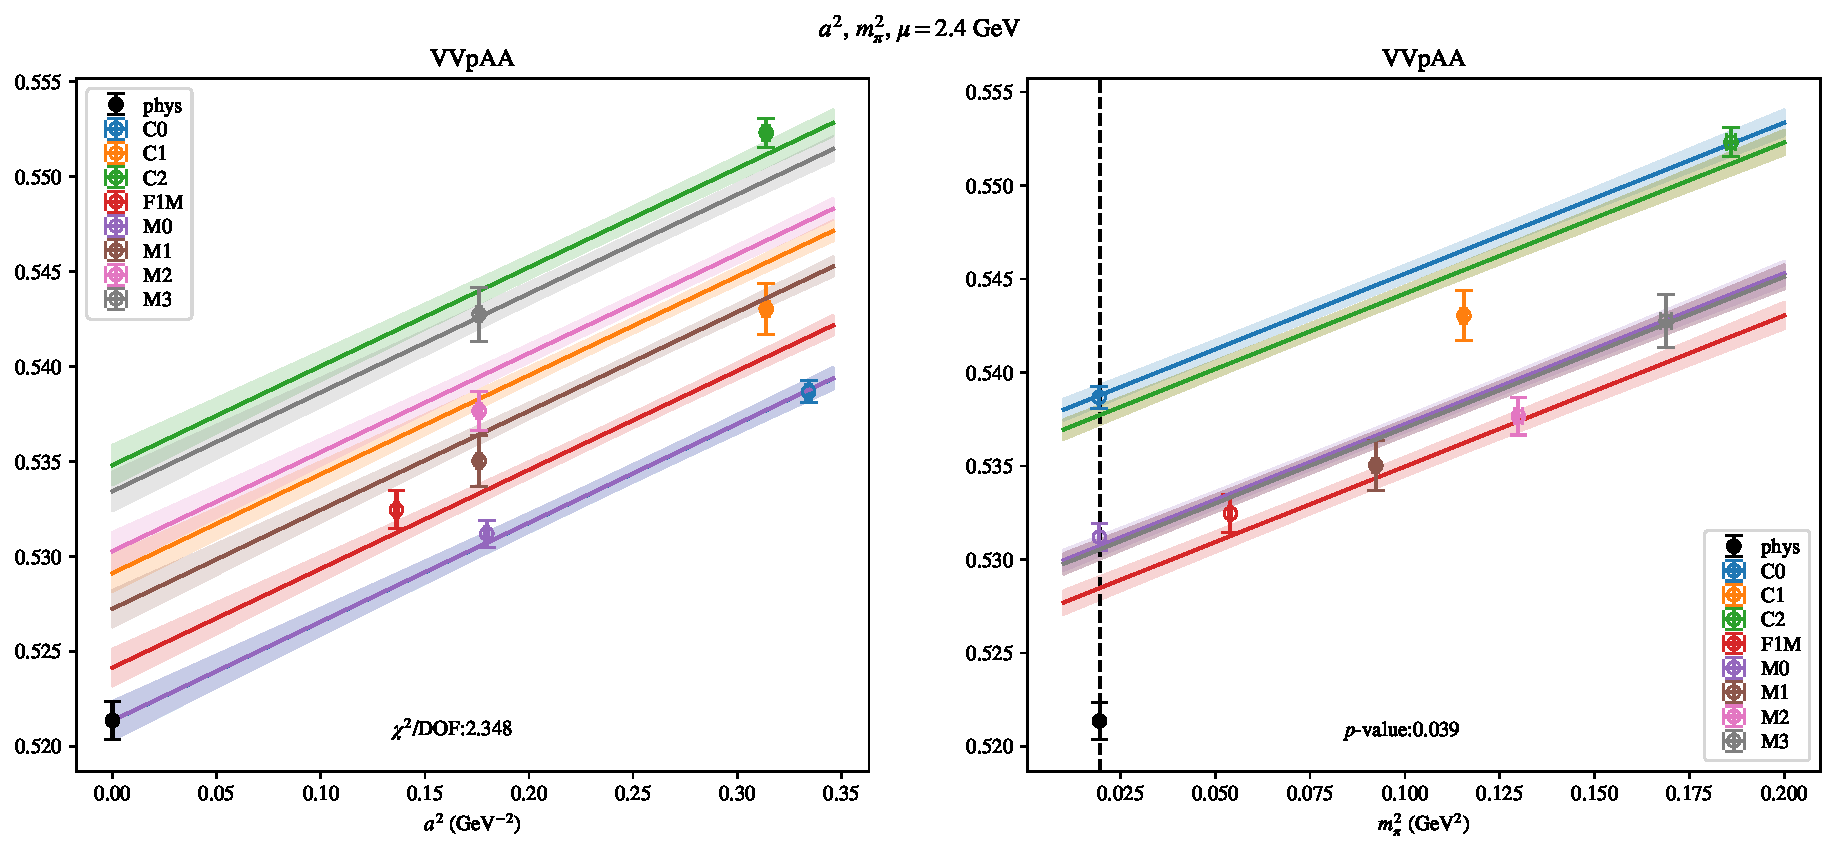
\includepdf[link, pages=-]{VVpAA/NPR/a2m2_24.pdf}
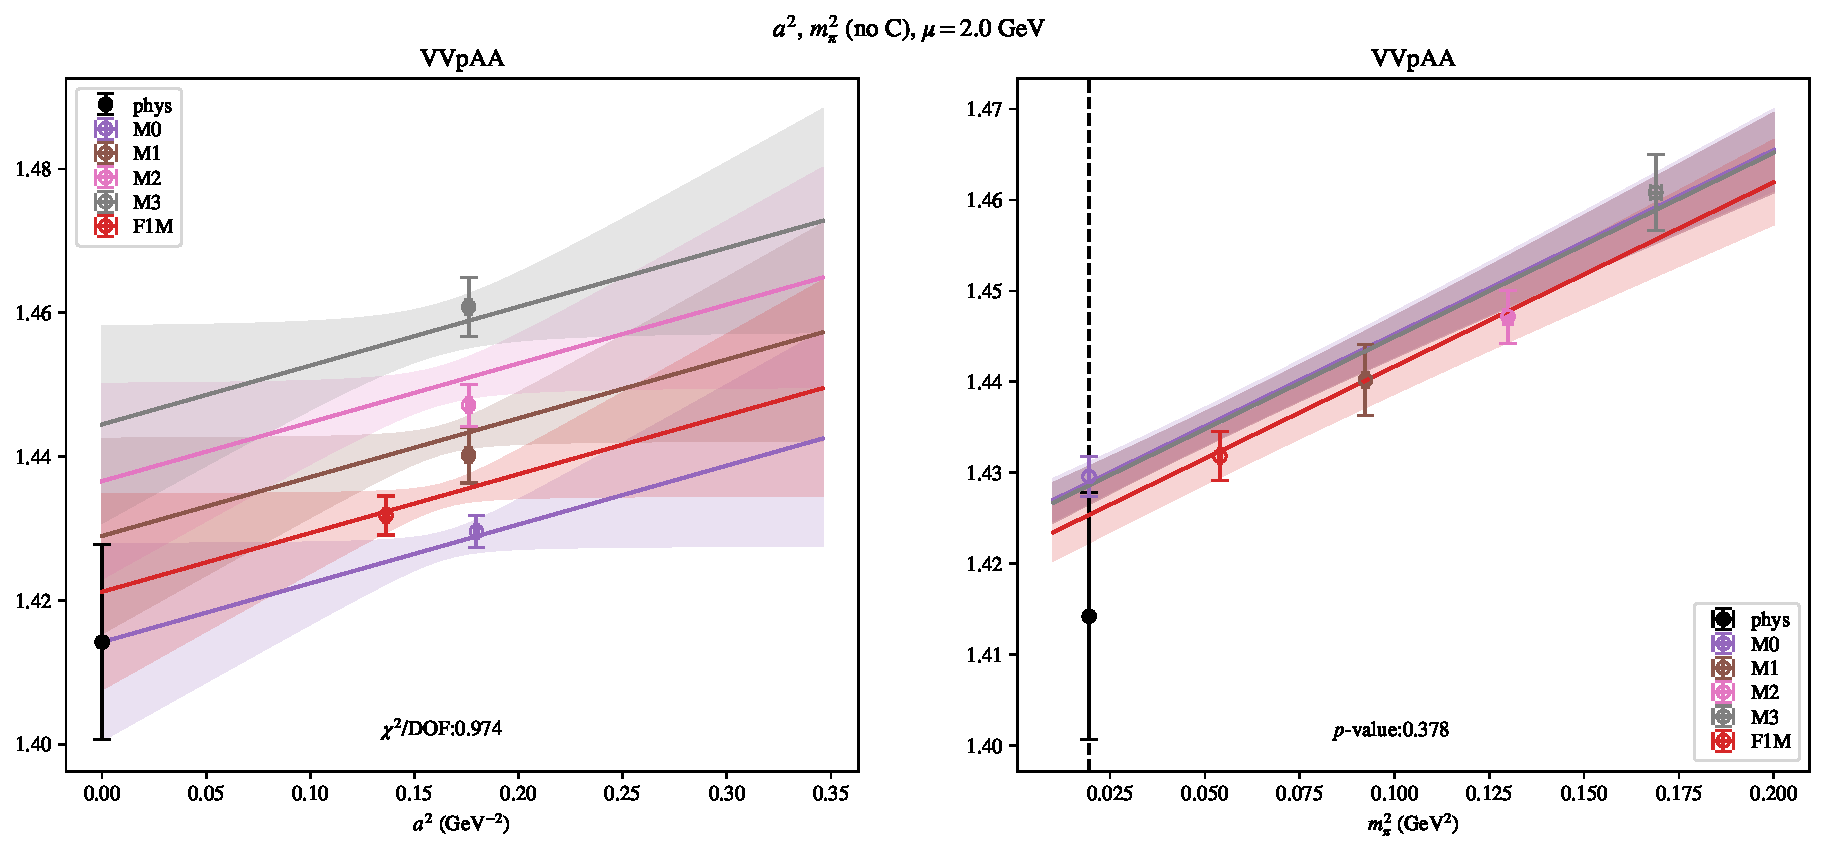
\includepdf[link, pages=-]{VVpAA/NPR/a2m2noC_20.pdf}
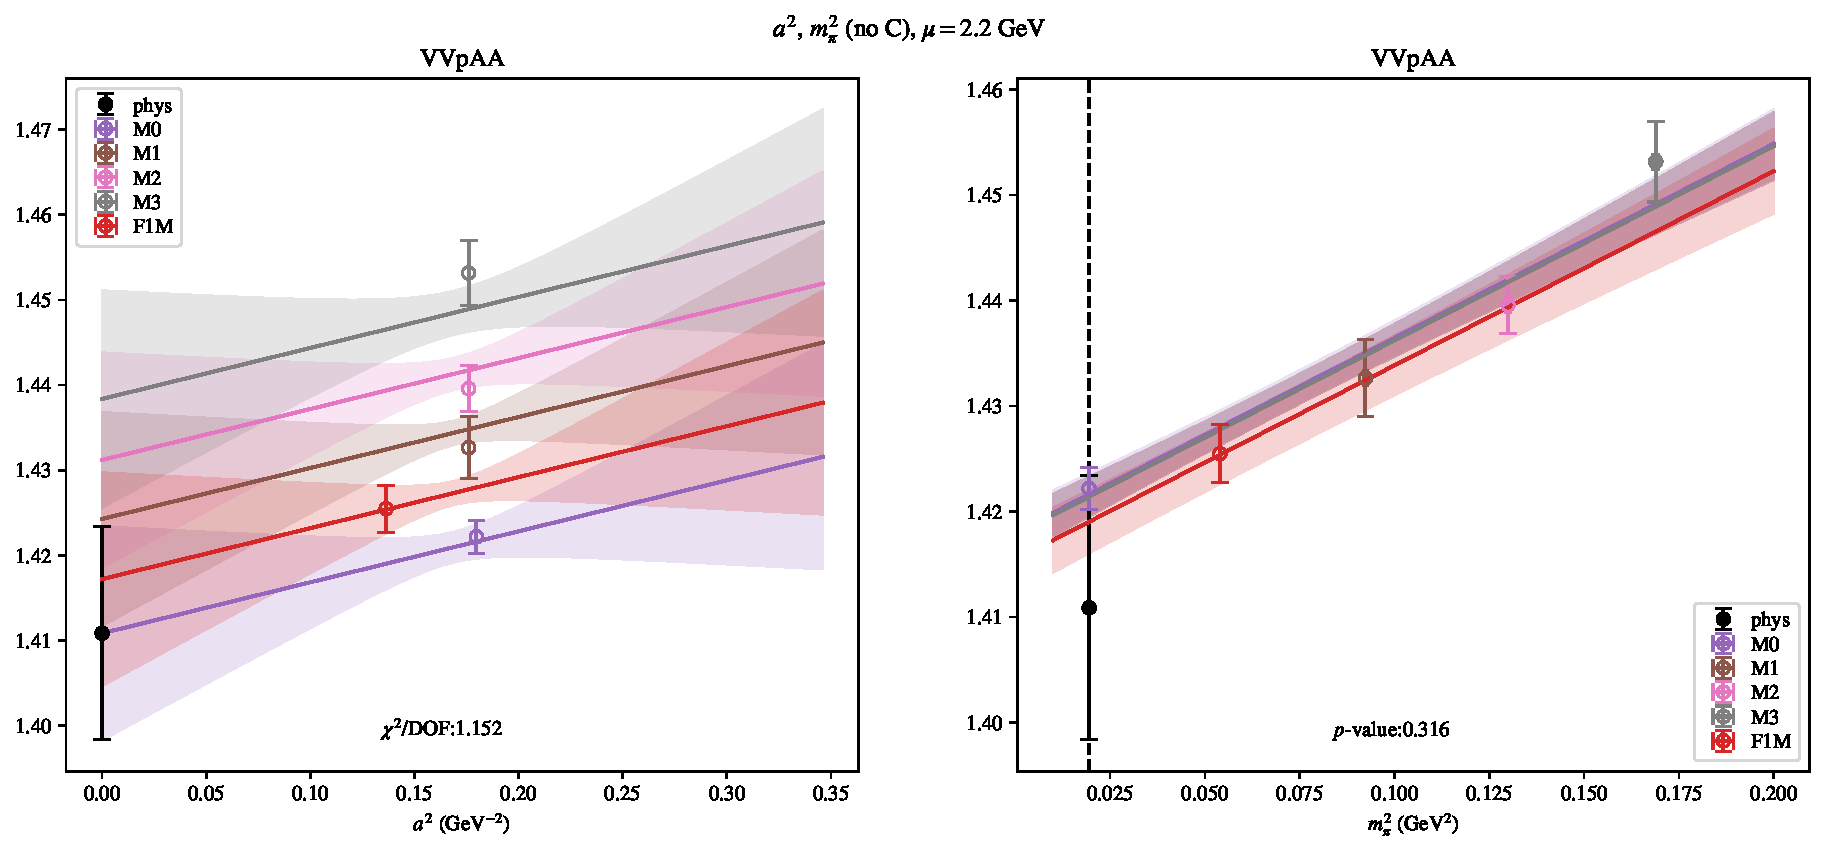
\includepdf[link, pages=-]{VVpAA/NPR/a2m2noC_22.pdf}
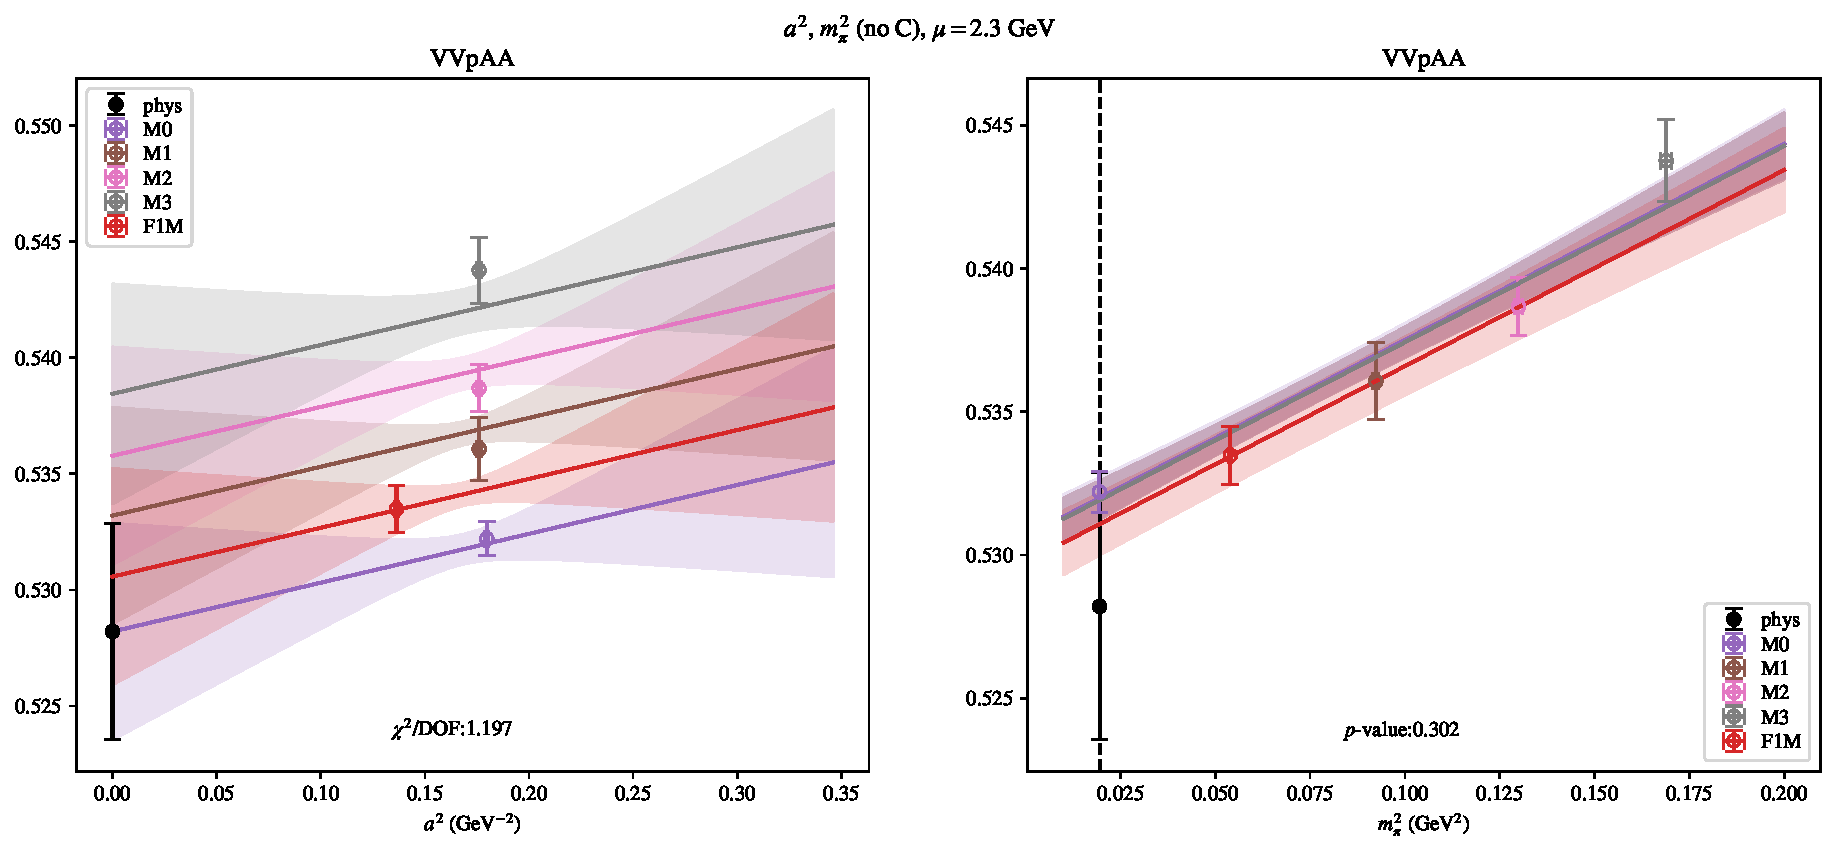
\includepdf[link, pages=-]{VVpAA/NPR/a2m2noC_23.pdf}
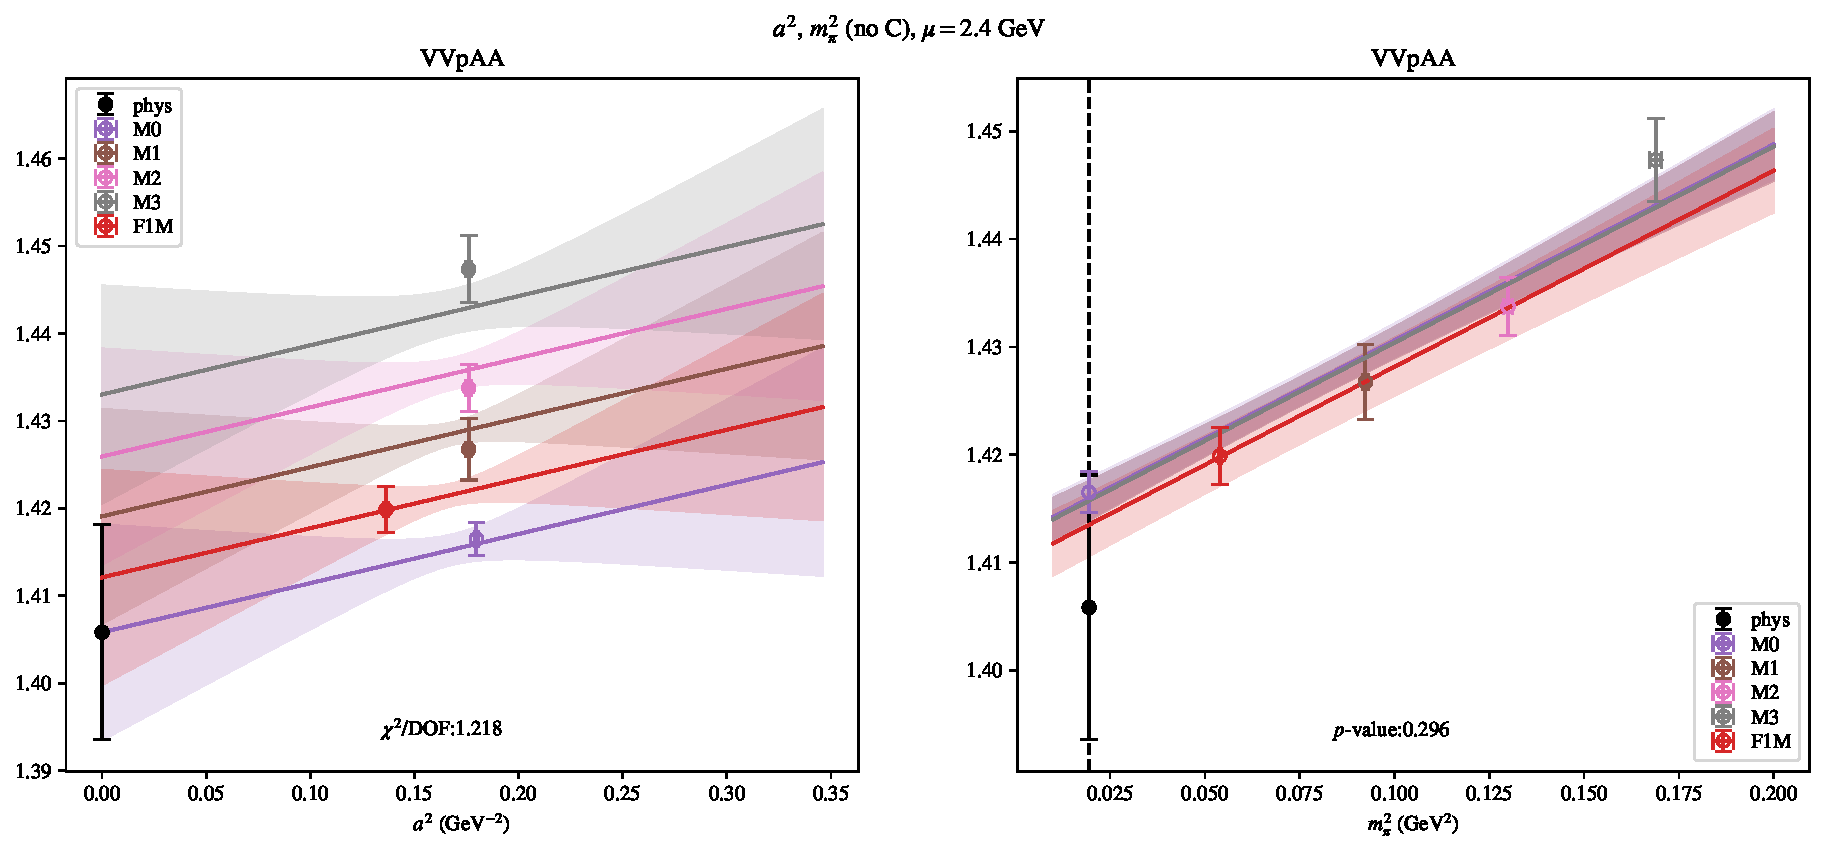
\includepdf[link, pages=-]{VVpAA/NPR/a2m2noC_24.pdf}
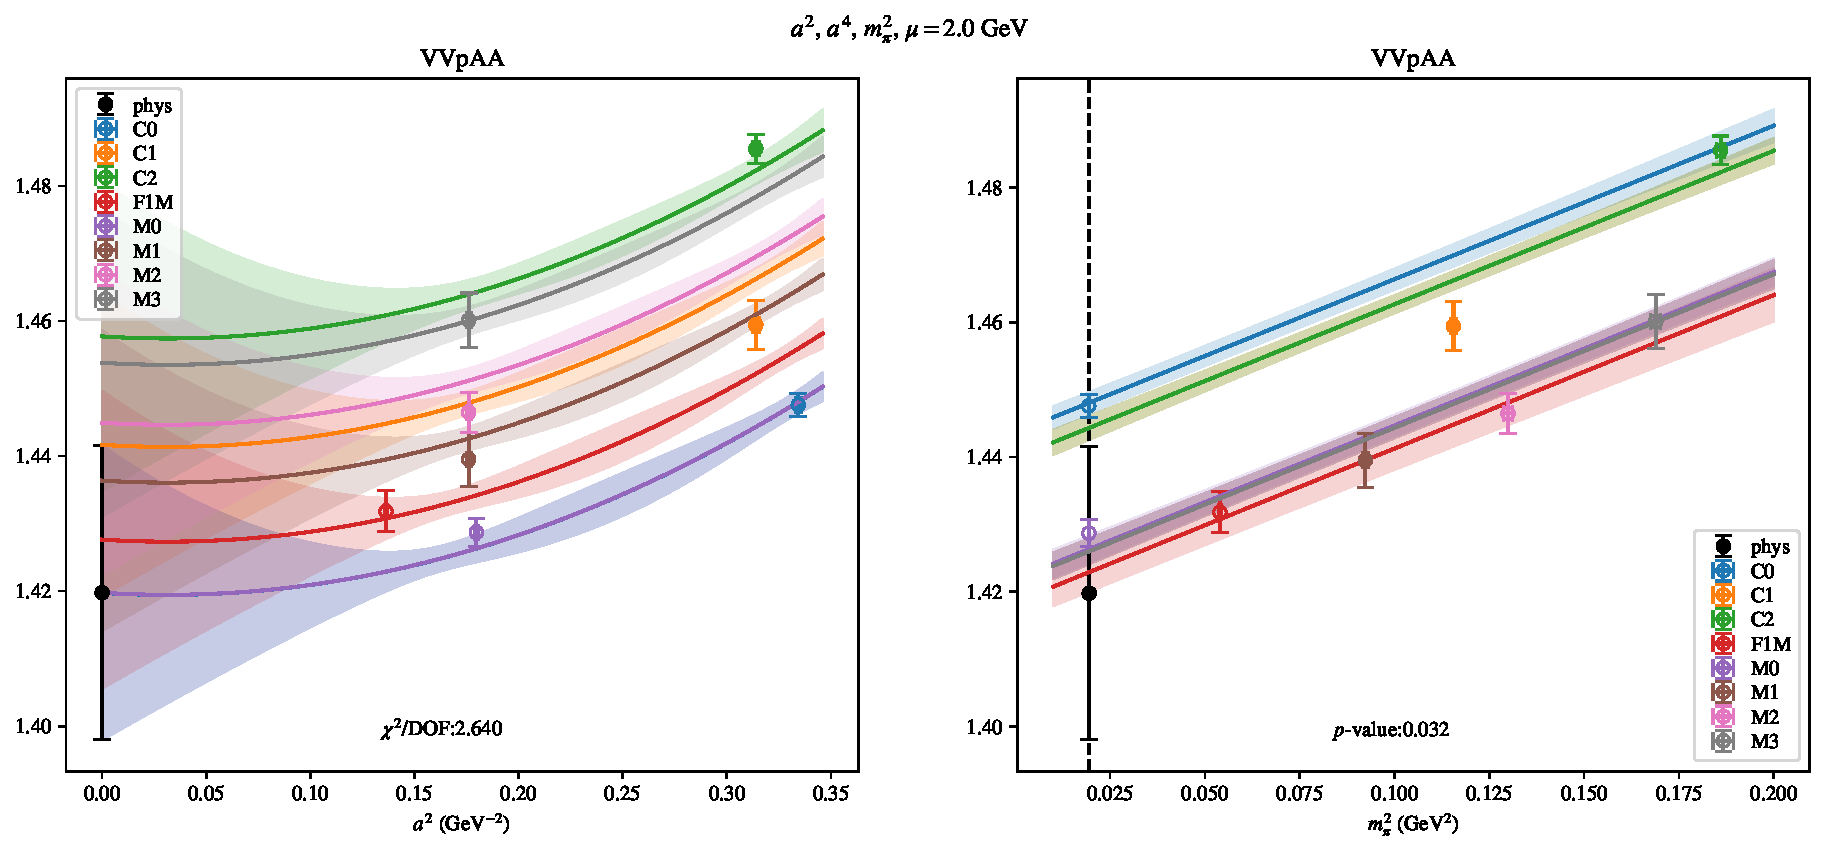
\includepdf[link, pages=-]{VVpAA/NPR/a2a4m2_20.pdf}
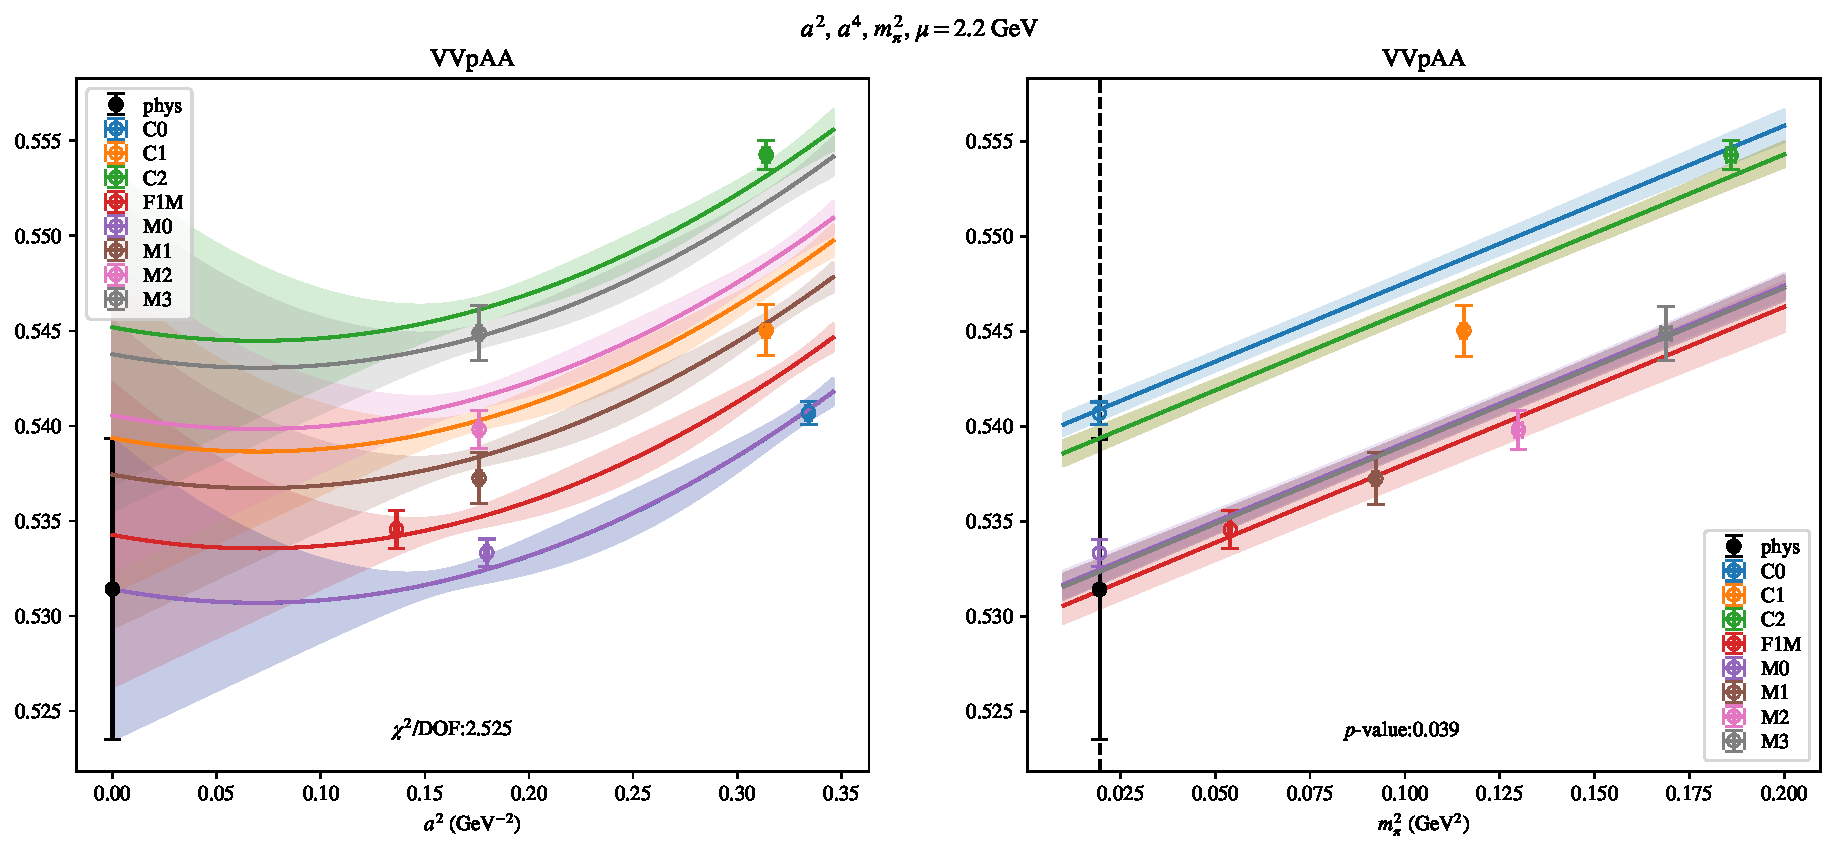
\includepdf[link, pages=-]{VVpAA/NPR/a2a4m2_22.pdf}
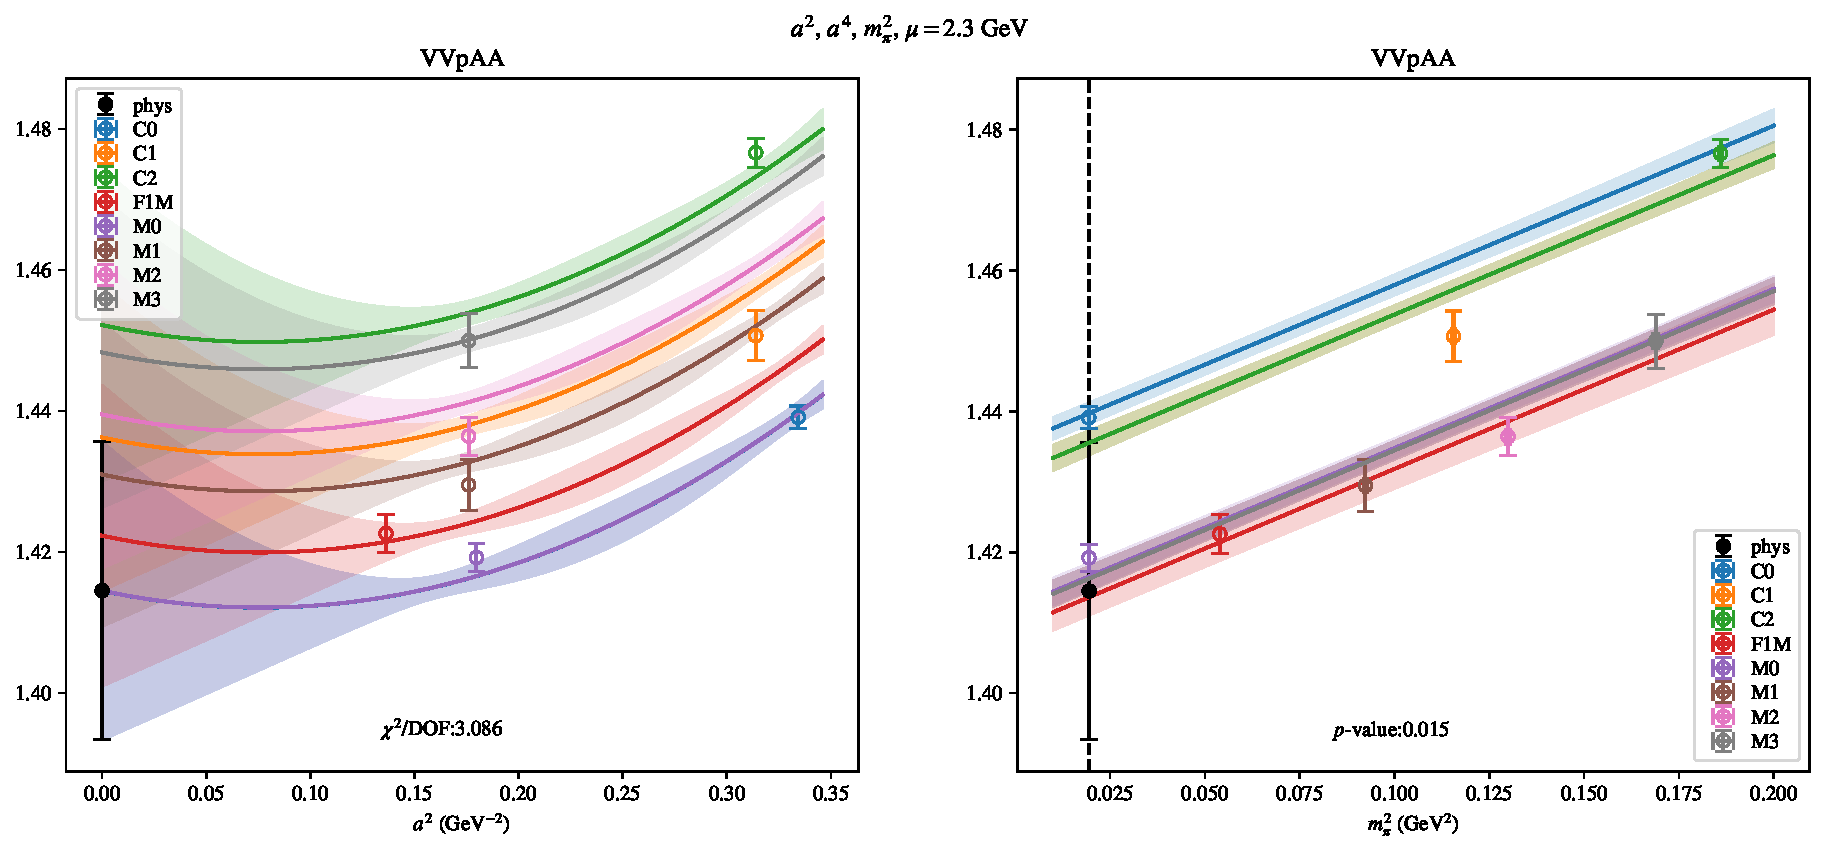
\includepdf[link, pages=-]{VVpAA/NPR/a2a4m2_23.pdf}
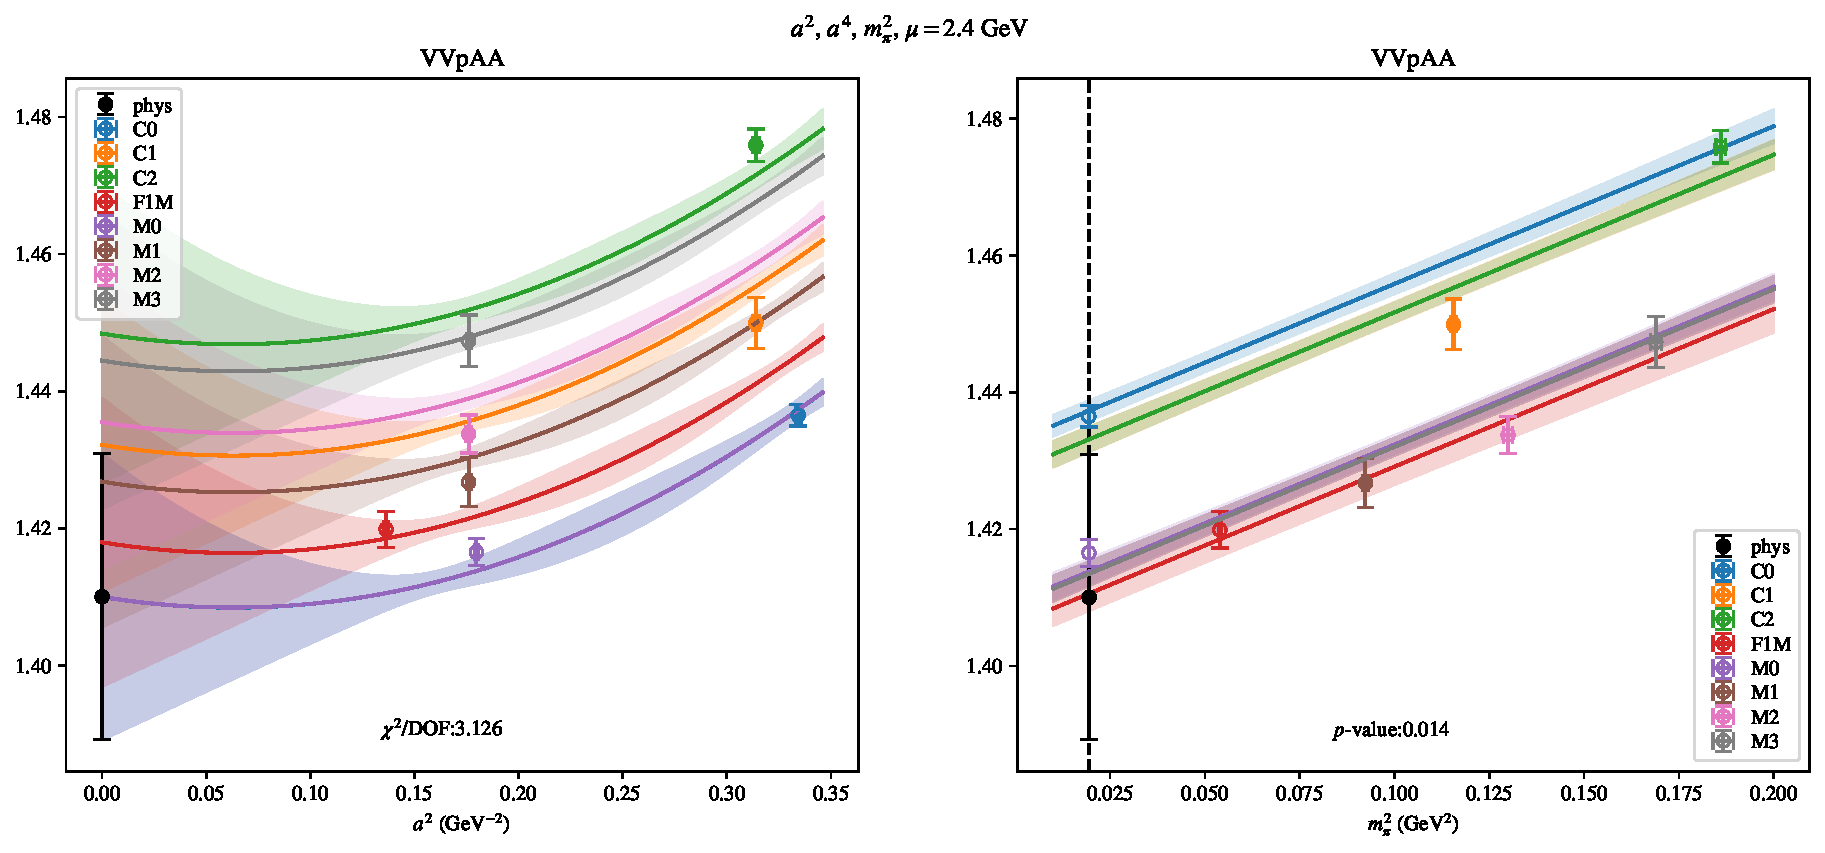
\includepdf[link, pages=-]{VVpAA/NPR/a2a4m2_24.pdf}
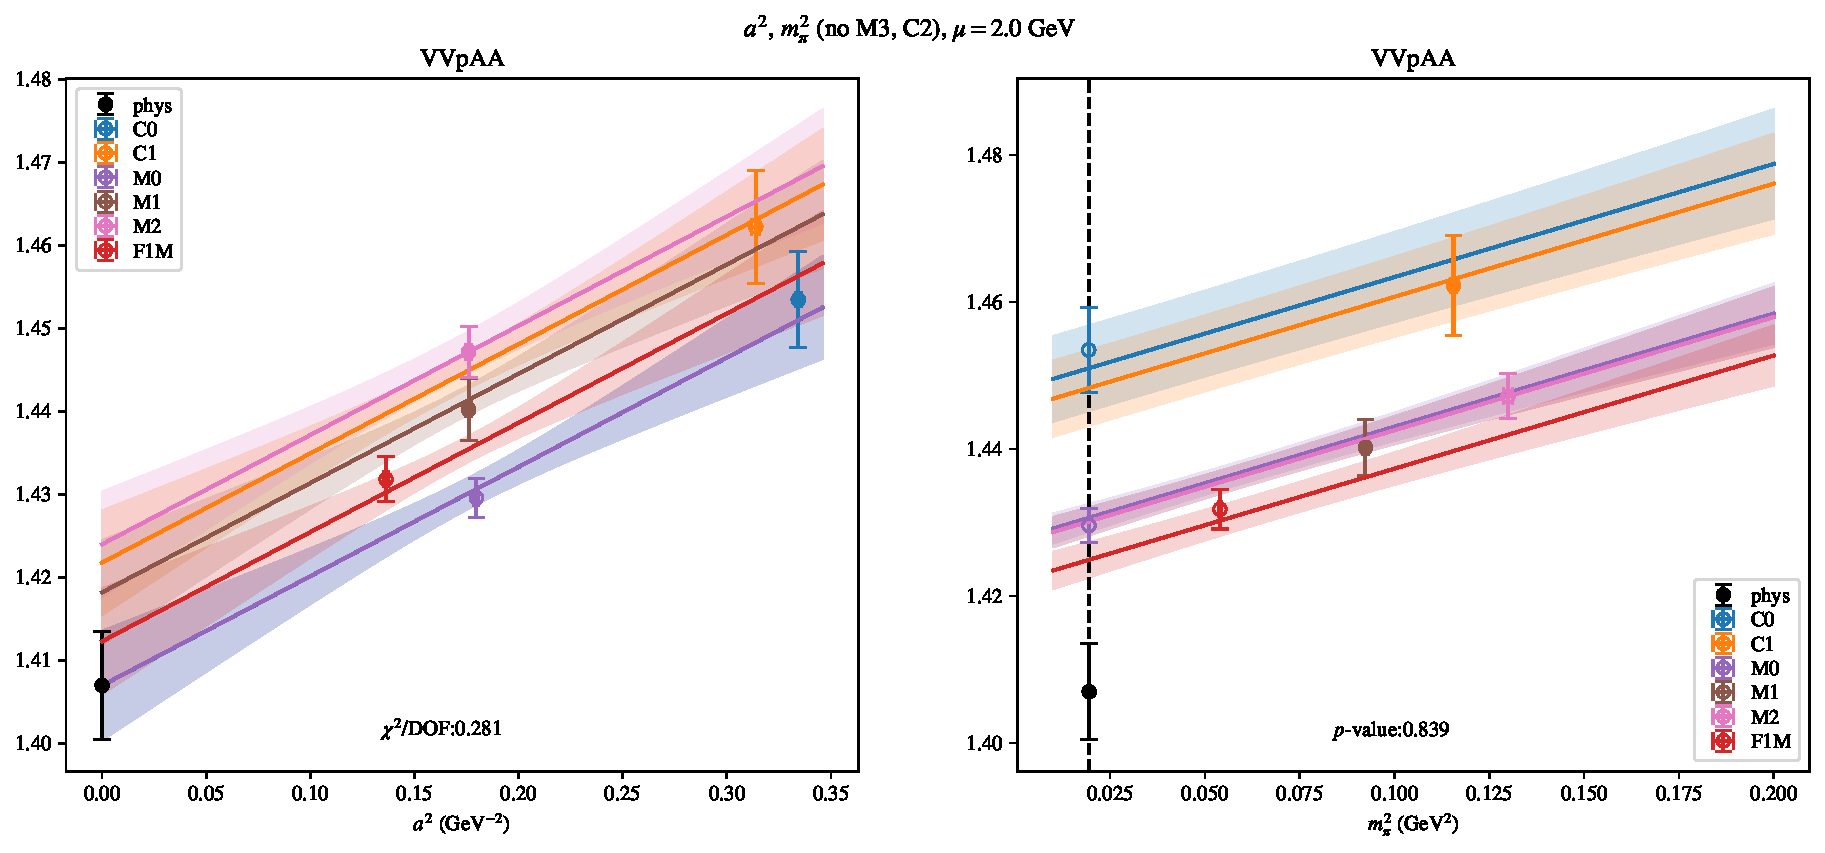
\includepdf[link, pages=-]{VVpAA/NPR/a2m2mcut_20.pdf}
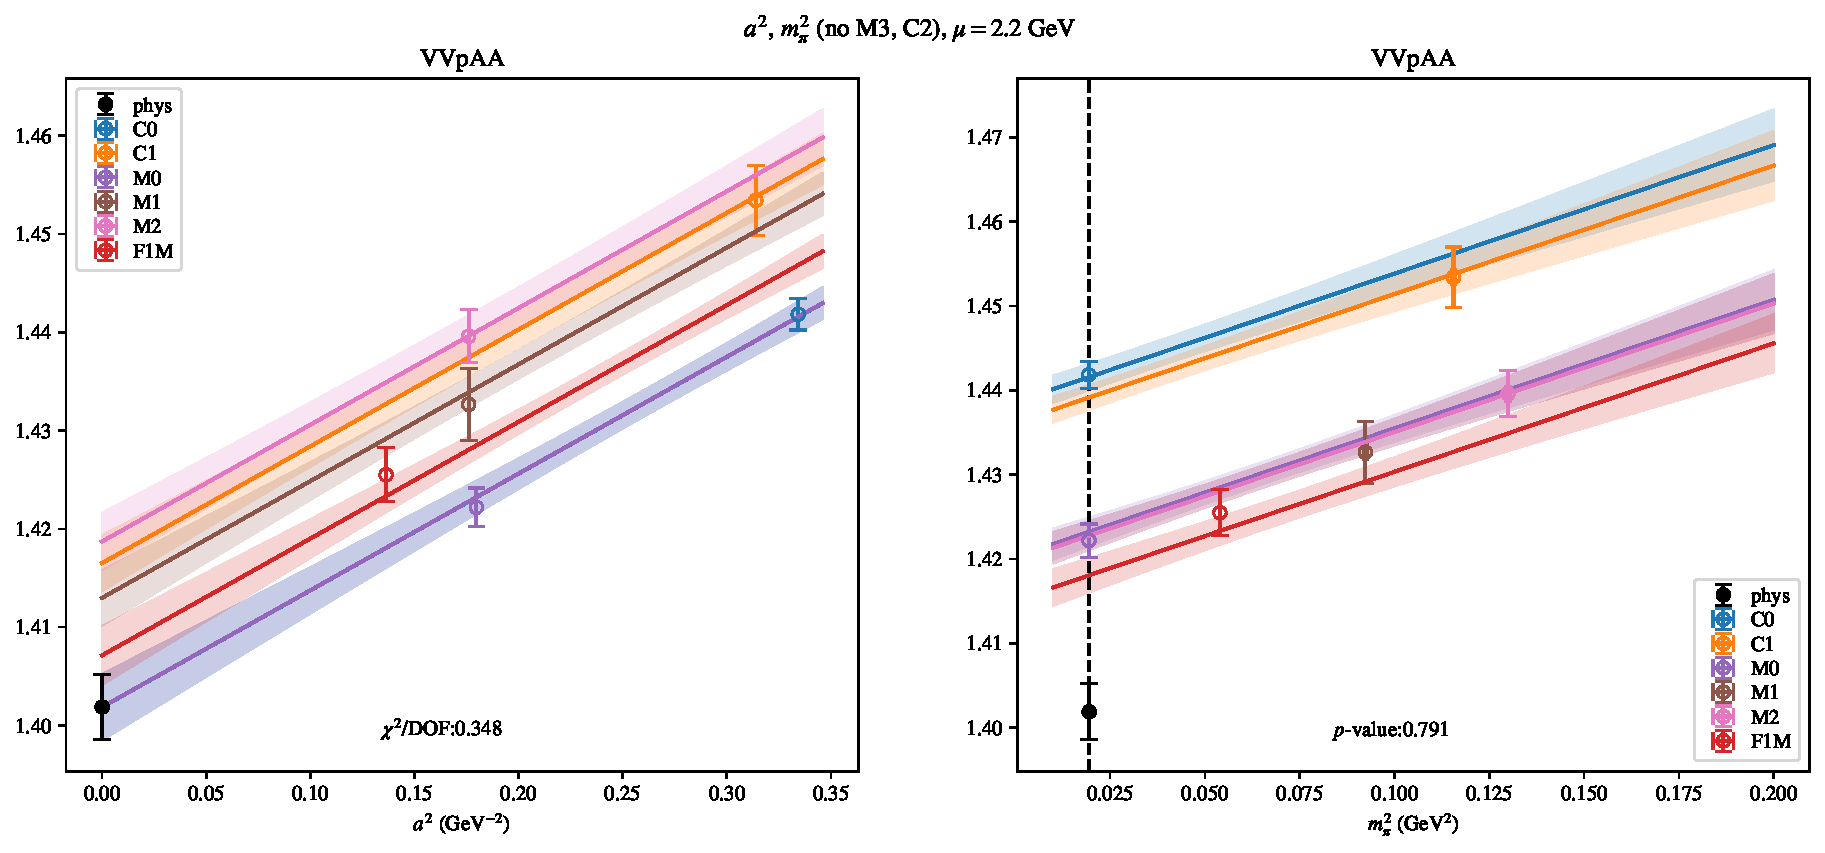
\includepdf[link, pages=-]{VVpAA/NPR/a2m2mcut_22.pdf}
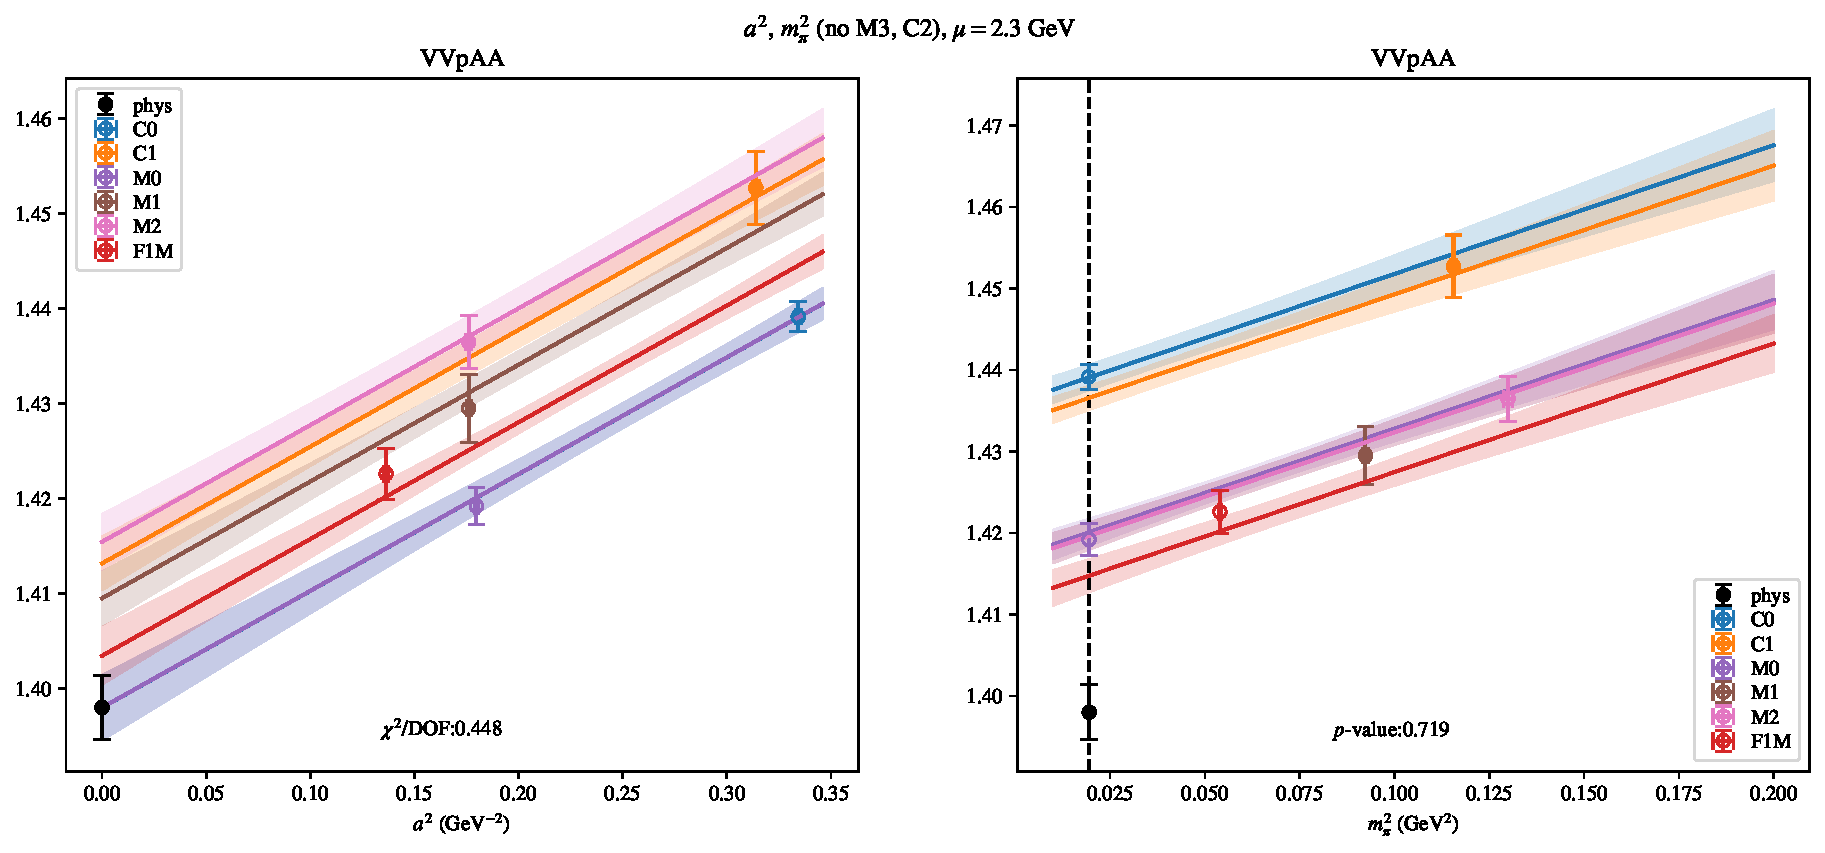
\includepdf[link, pages=-]{VVpAA/NPR/a2m2mcut_23.pdf}
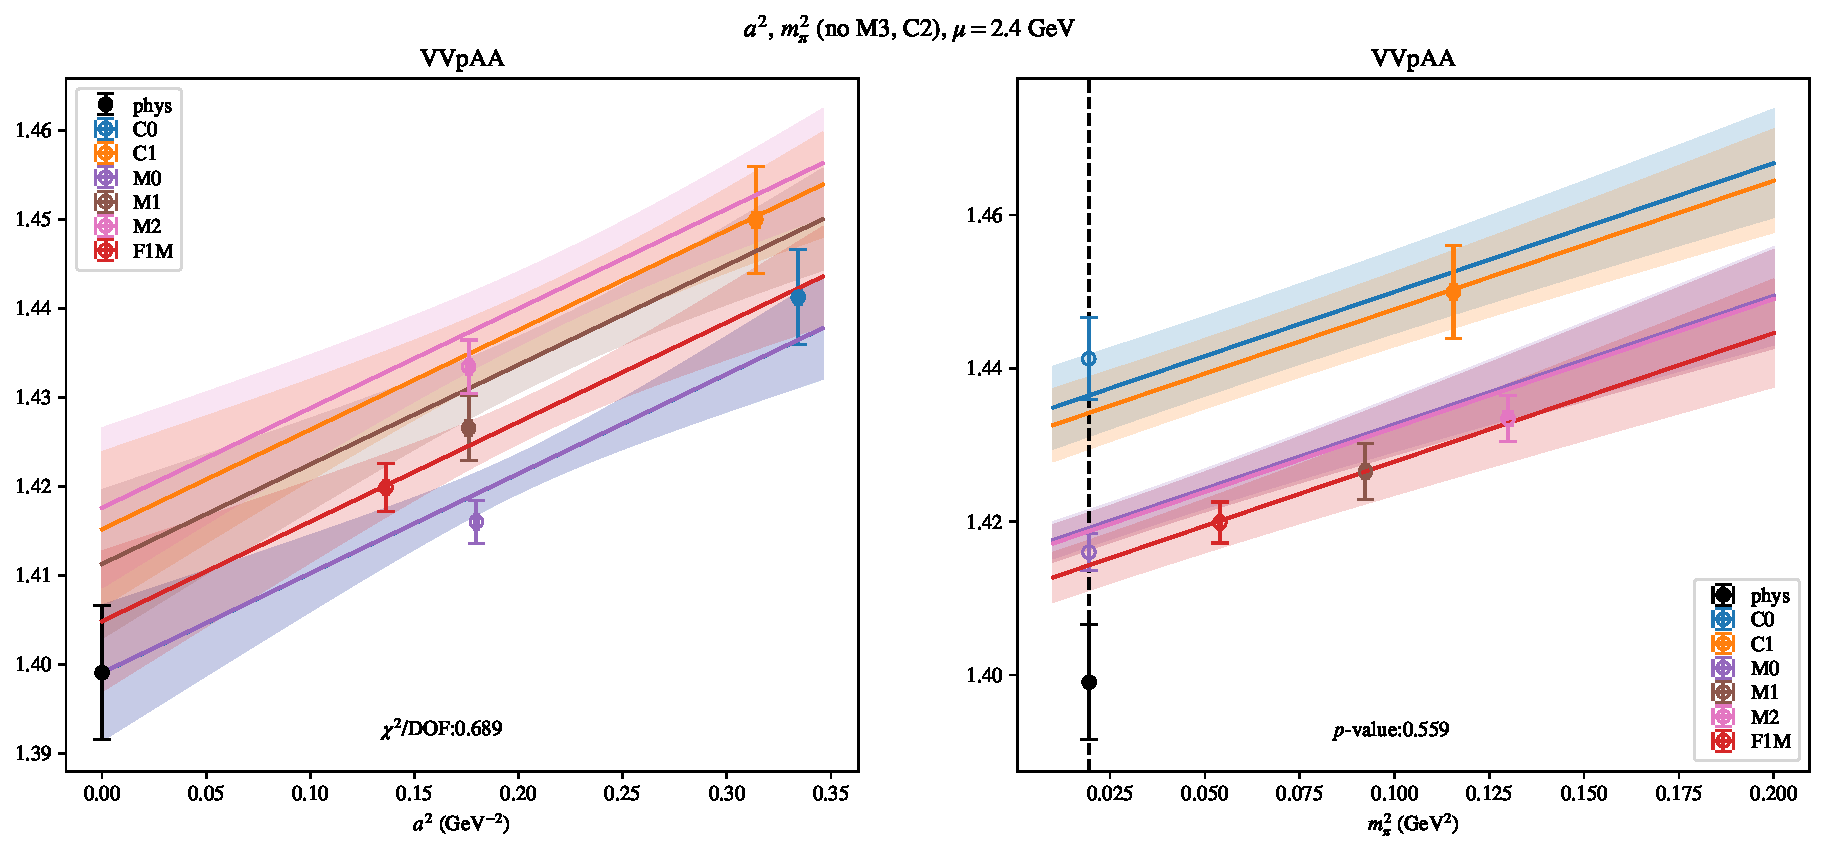
\includepdf[link, pages=-]{VVpAA/NPR/a2m2mcut_24.pdf}
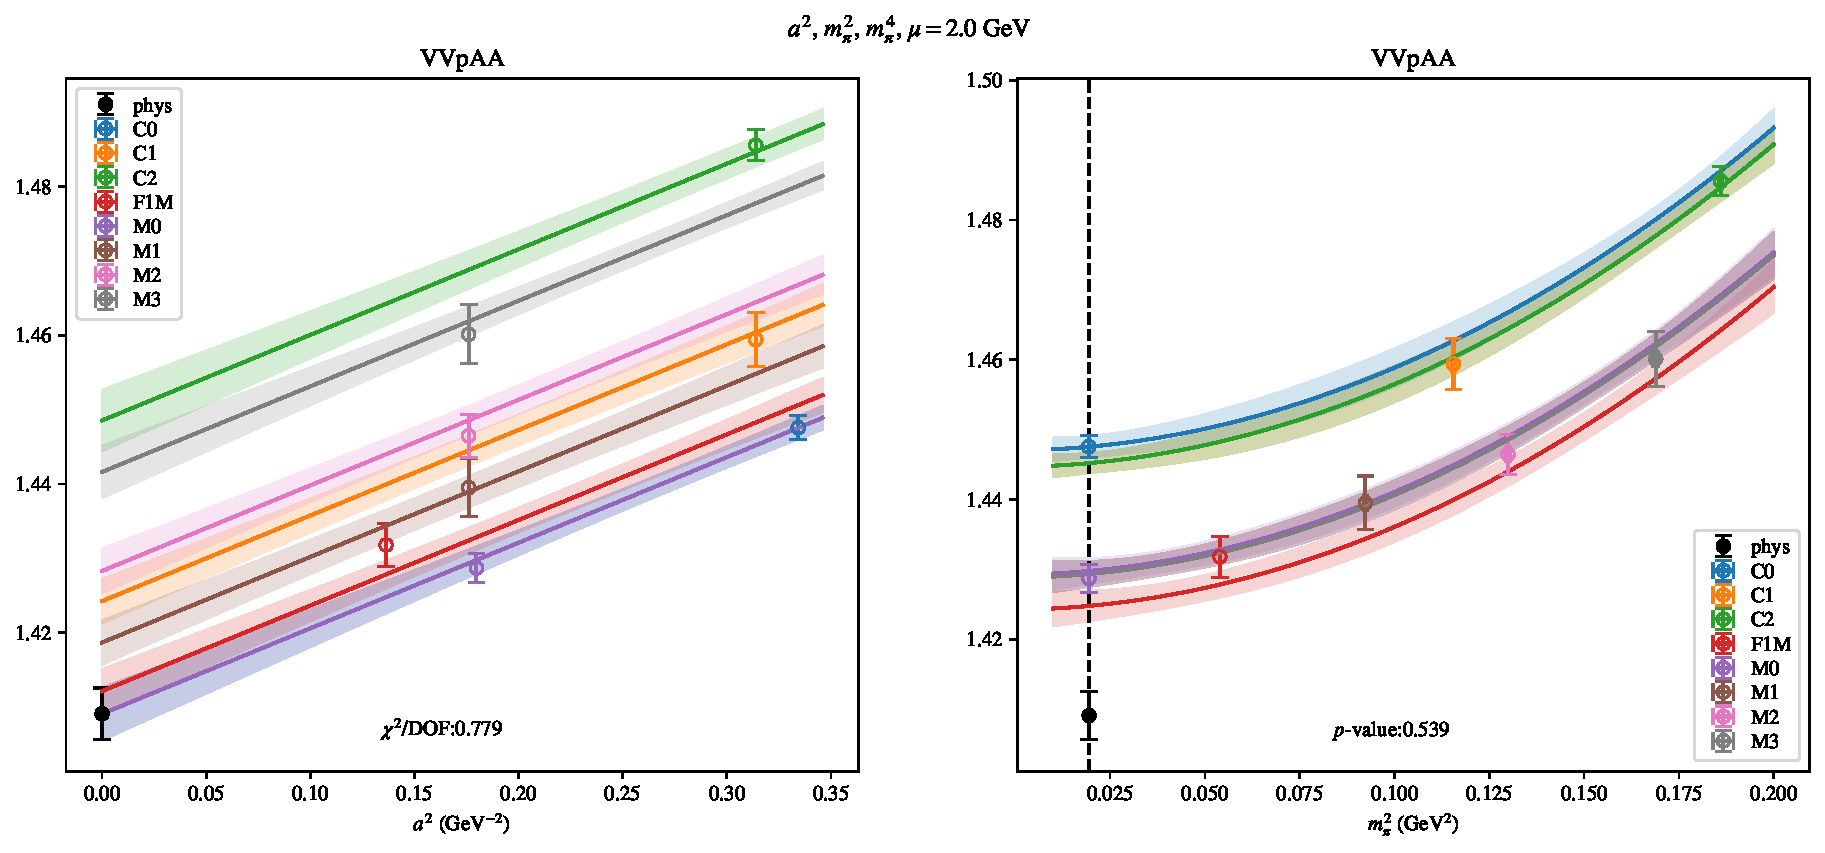
\includepdf[link, pages=-]{VVpAA/NPR/a2m2m4_20.pdf}
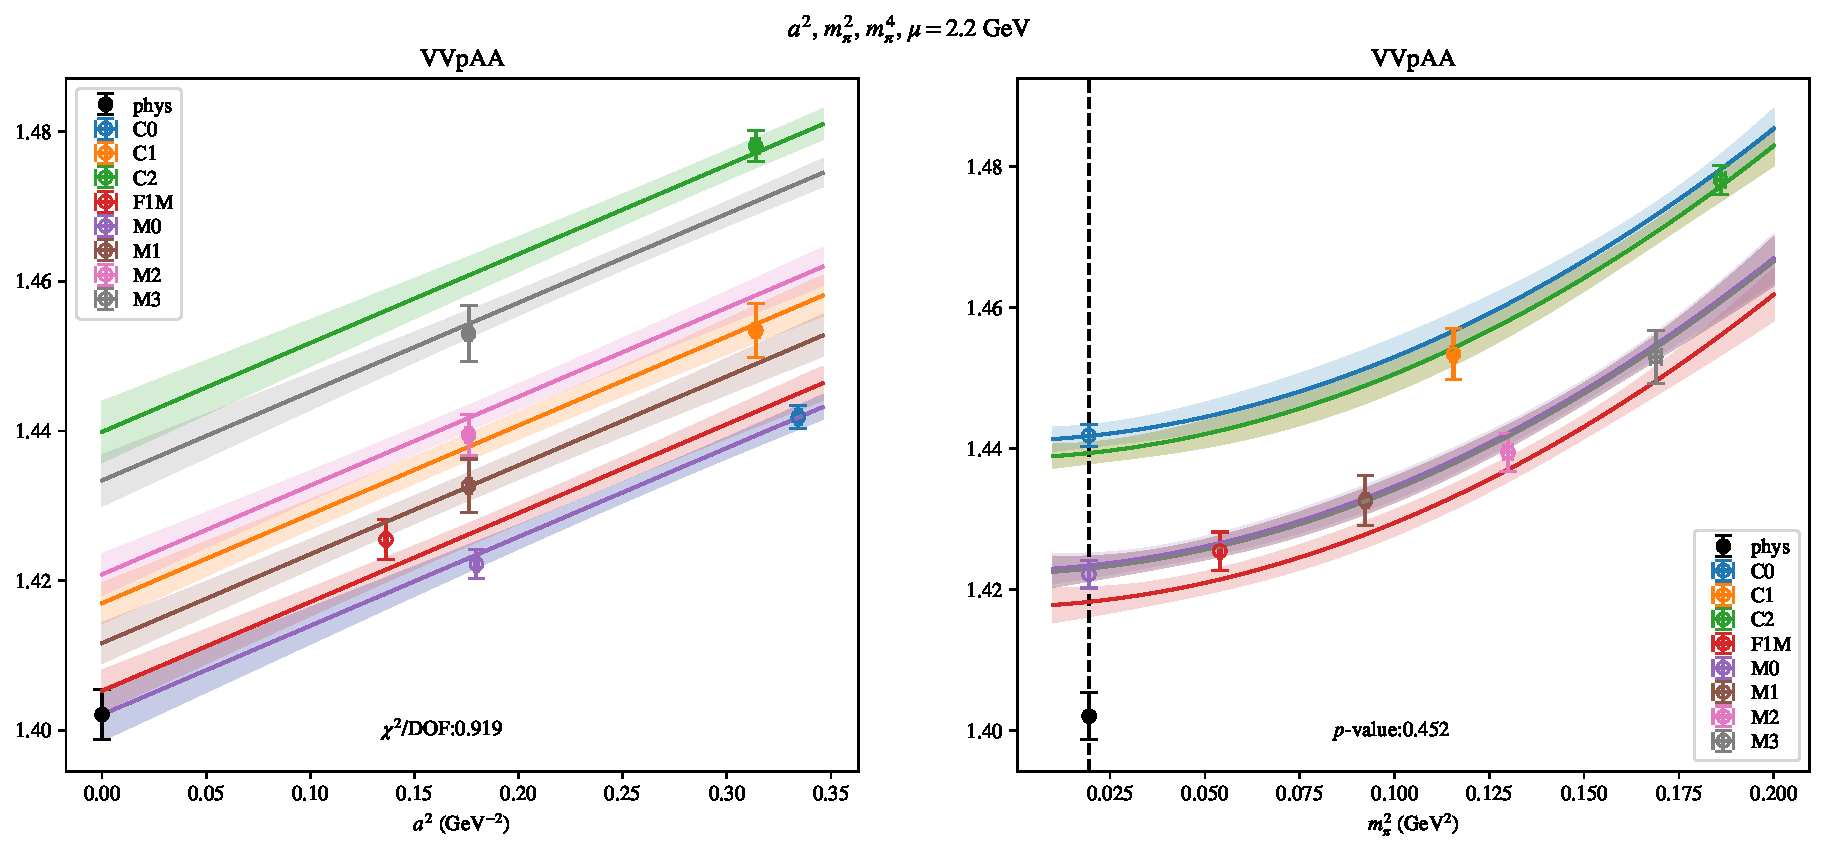
\includepdf[link, pages=-]{VVpAA/NPR/a2m2m4_22.pdf}
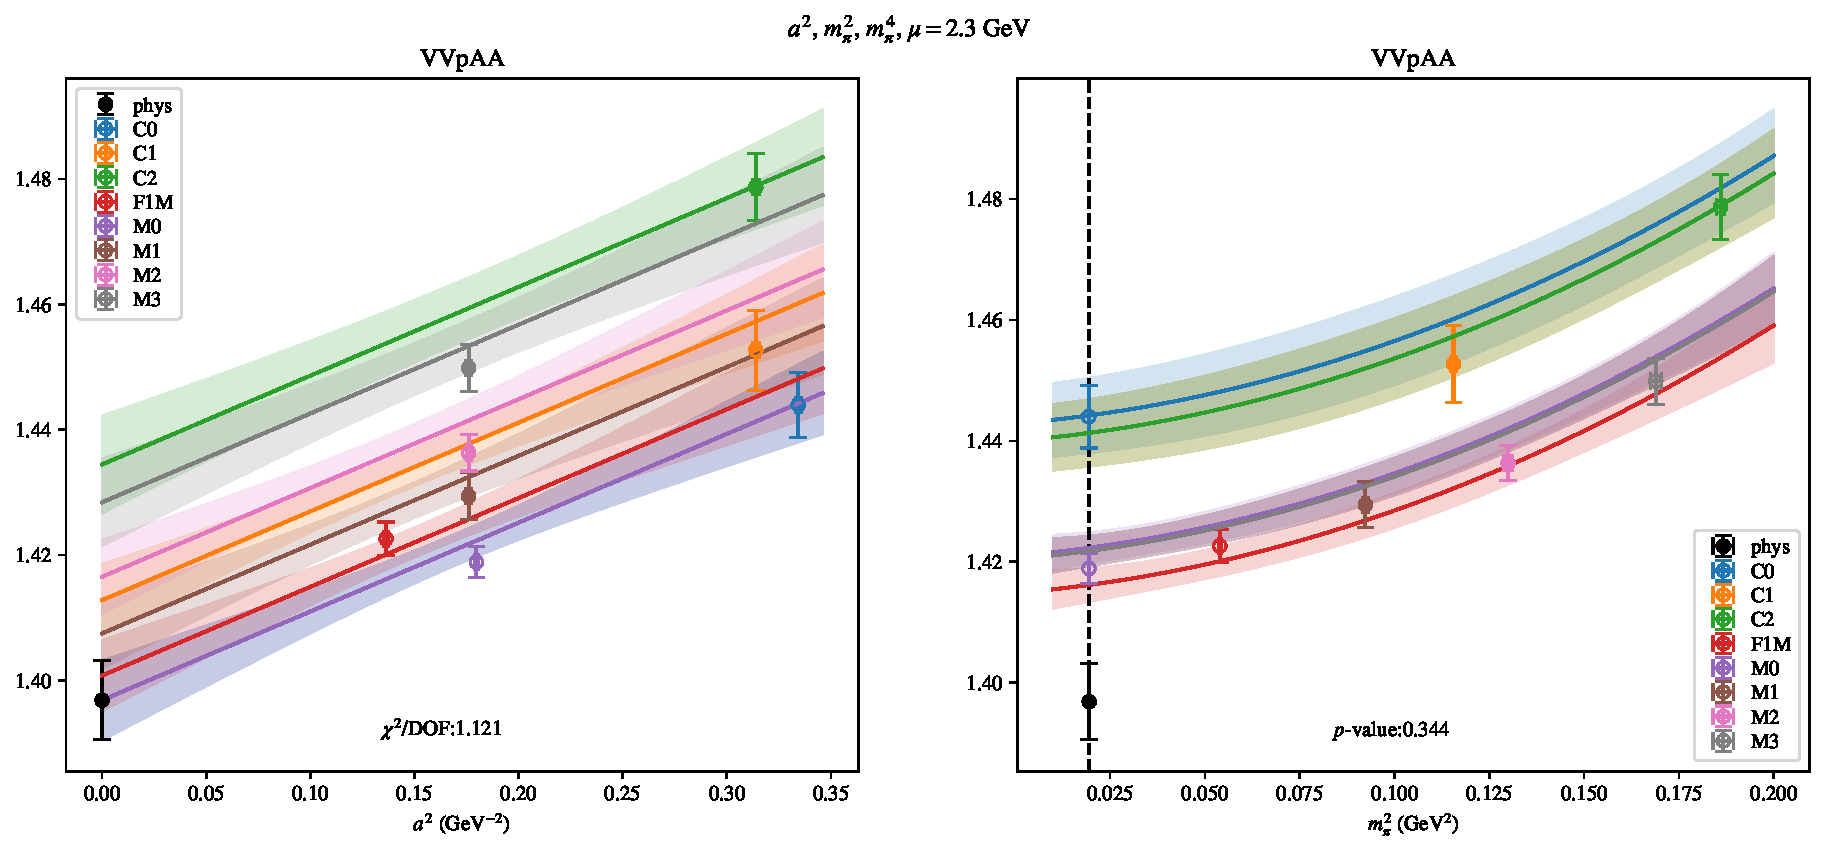
\includepdf[link, pages=-]{VVpAA/NPR/a2m2m4_23.pdf}
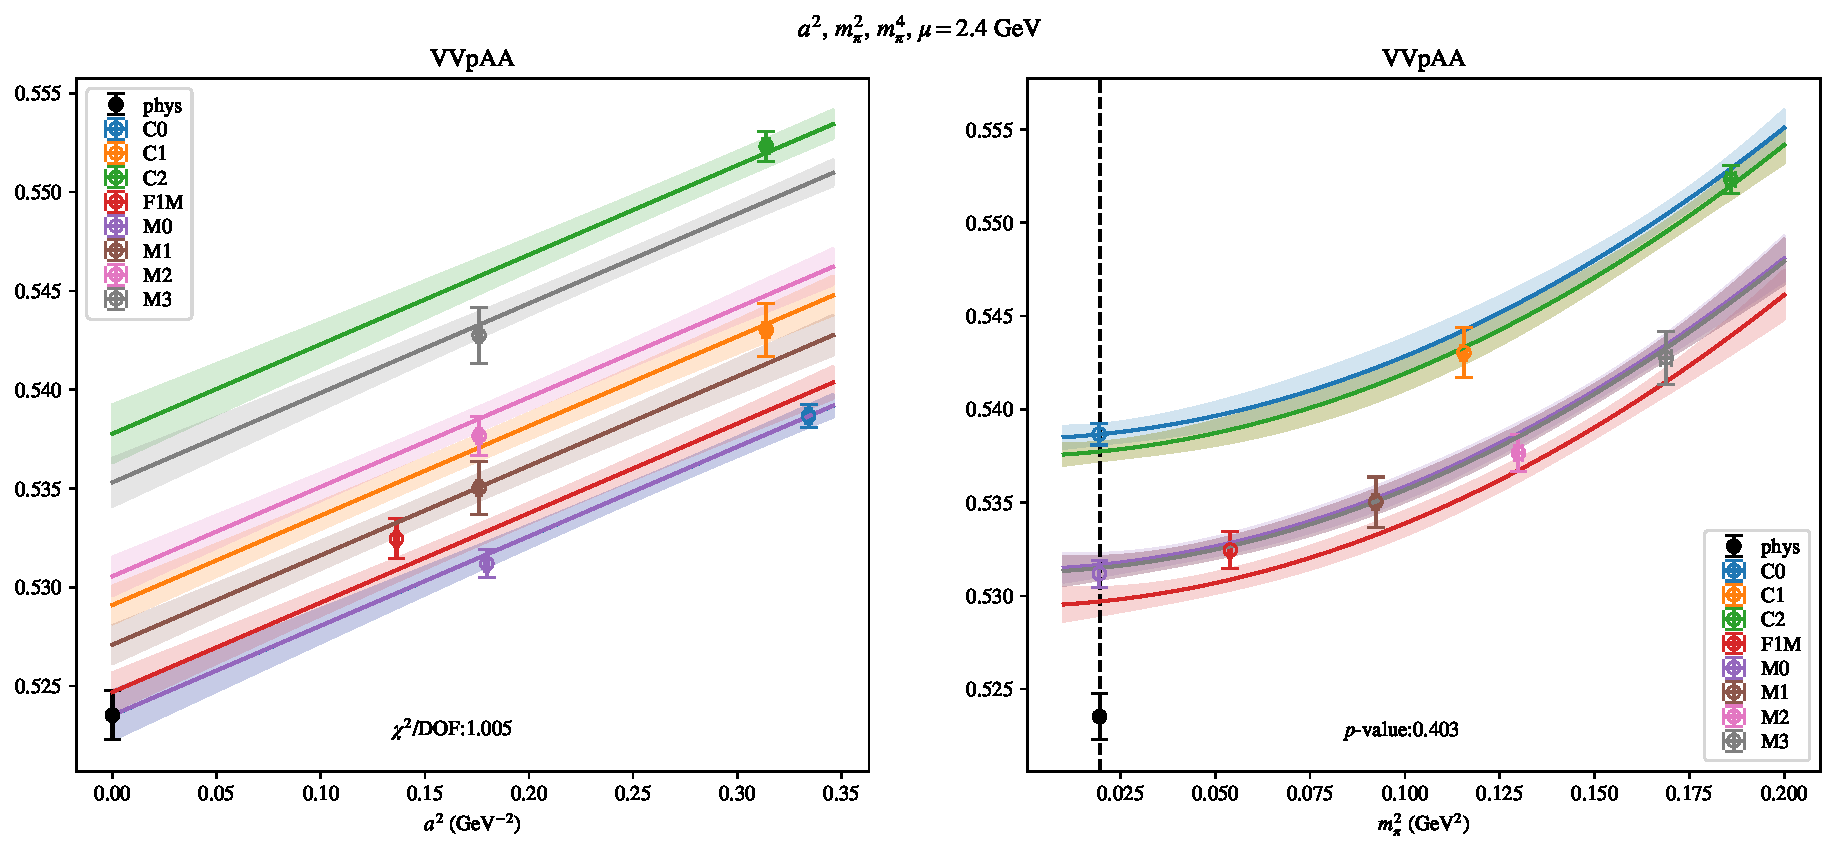
\includepdf[link, pages=-]{VVpAA/NPR/a2m2m4_24.pdf}
\clearpage
\section{$\mathcal{B}_2$}
\begin{table}[h!]
\begin{center}
\begin{tabular}{|c|c|c|c|c|c|}
\hline
$\mu$ (GeV) & $a^2$, $m_\pi^2$& $a^2$, $m_\pi^2$ (no C)& $a^2$, $a^4$, $m_\pi^2$& $a^2$, $m_\pi^2$ (no M3, C2)& $a^2$, $m_\pi^2$, $m_\pi^4$\\
\hline
2.0& \hyperlink{VVmAA/NPR/a2m2_20.pdf.1}{\textbf{-0.991(15)}: 10.213 (0.0)} & \hyperlink{VVmAA/NPR/a2m2noC_20.pdf.1}{\textbf{-0.931(92)}: 1.858 (0.156)} & \hyperlink{VVmAA/NPR/a2a4m2_20.pdf.1}{\textbf{-0.89(13)}: 1.848 (0.117)} & \hyperlink{VVmAA/NPR/a2m2mcut_20.pdf.1}{\textbf{-0.992(15)}: 16.011 (0.0)} & \hyperlink{VVmAA/NPR/a2m2m4_20.pdf.1}{\textbf{-0.993(16)}: 9.846 (0.0)}\\
2.2& \hyperlink{VVmAA/NPR/a2m2_22.pdf.1}{\textbf{-1.005(15)}: 9.863 (0.0)} & \hyperlink{VVmAA/NPR/a2m2noC_22.pdf.1}{\textbf{-0.950(90)}: 2.946 (0.053)} & \hyperlink{VVmAA/NPR/a2a4m2_22.pdf.1}{\textbf{-0.92(13)}: 2.585 (0.035)} & \hyperlink{VVmAA/NPR/a2m2mcut_22.pdf.1}{\textbf{-1.006(15)}: 13.946 (0.0)} & \hyperlink{VVmAA/NPR/a2m2m4_22.pdf.1}{\textbf{-1.007(15)}: 8.397 (0.0)}\\
2.3& \hyperlink{VVmAA/NPR/a2m2_23.pdf.1}{\textbf{-1.012(15)}: 10.017 (0.0)} & \hyperlink{VVmAA/NPR/a2m2noC_23.pdf.1}{\textbf{-0.956(88)}: 3.134 (0.044)} & \hyperlink{VVmAA/NPR/a2a4m2_23.pdf.1}{\textbf{-0.92(13)}: 2.463 (0.043)} & \hyperlink{VVmAA/NPR/a2m2mcut_23.pdf.1}{\textbf{-1.012(15)}: 14.356 (0.0)} & \hyperlink{VVmAA/NPR/a2m2m4_23.pdf.1}{\textbf{-1.014(15)}: 8.831 (0.0)}\\
2.4& \hyperlink{VVmAA/NPR/a2m2_24.pdf.1}{\textbf{-1.016(15)}: 9.213 (0.0)} & \hyperlink{VVmAA/NPR/a2m2noC_24.pdf.1}{\textbf{-0.964(86)}: 3.097 (0.045)} & \hyperlink{VVmAA/NPR/a2a4m2_24.pdf.1}{\textbf{-0.93(13)}: 2.627 (0.033)} & \hyperlink{VVmAA/NPR/a2m2mcut_24.pdf.1}{\textbf{-1.017(15)}: 13.074 (0.0)} & \hyperlink{VVmAA/NPR/a2m2m4_24.pdf.1}{\textbf{-1.018(15)}: 8.22 (0.0)}\\
\hline
\end{tabular}
\caption{Physical point value from chiral and continuum extrapolation at renormalisation scale $\mu$. Entries are \textbf{value(error)}: $\chi^2/\text{DOF}$ ($p$-value).}
\end{center}
\end{table}
\begin{table}[h!]
\begin{center}
\begin{tabular}{|c c|c|c|c|c|c|}
\hline
$\mu$ (GeV) &  & $a^2$, $m_\pi^2$& $a^2$, $m_\pi^2$ (no C)& $a^2$, $a^4$, $m_\pi^2$& $a^2$, $m_\pi^2$ (no M3, C2)& $a^2$, $m_\pi^2$, $m_\pi^4$\\
\hline
\multirow{2}{0.5in}{2.0} & $\alpha$ & -0.183(57)& 0.176(58)& 0.71(14)& -0.185(56)& -0.189(57)\\
 & $\beta$ & 0.00106(15)& 0.00114(25)& 0.00085(18)& 0.00072(25)& -0.0013(78)\\
\hline
\multirow{2}{0.5in}{2.2} & $\alpha$ & -0.224(55)& 0.099(55)& 0.57(14)& -0.225(54)& -0.229(55)\\
 & $\beta$ & 0.00117(13)& 0.00120(23)& 0.00098(16)& 0.00068(23)& -0.0013(71)\\
\hline
\multirow{2}{0.5in}{2.3} & $\alpha$ & -0.246(55)& 0.070(53)& 0.54(13)& -0.247(54)& -0.252(55)\\
 & $\beta$ & 0.00117(13)& 0.00119(22)& 0.00098(16)& 0.00071(23)& -0.0012(70)\\
\hline
\multirow{2}{0.5in}{2.4} & $\alpha$ & -0.265(54)& 0.031(51)& 0.45(13)& -0.266(54)& -0.271(55)\\
 & $\beta$ & 0.00112(13)& 0.00120(21)& 0.00095(15)& 0.00070(22)& -0.0010(68)\\
\hline
\end{tabular}
\caption{Fit values of coefficients in $Q = Q_{phys} + \mathbf{\alpha} a^2 + \mathbf{\beta}\left(\frac{m_\pi^2}{f_\pi^2}-\frac{m_{\pi,PDG}^2}{f_\pi^2}\right) + \ldots$.}
\end{center}
\end{table}
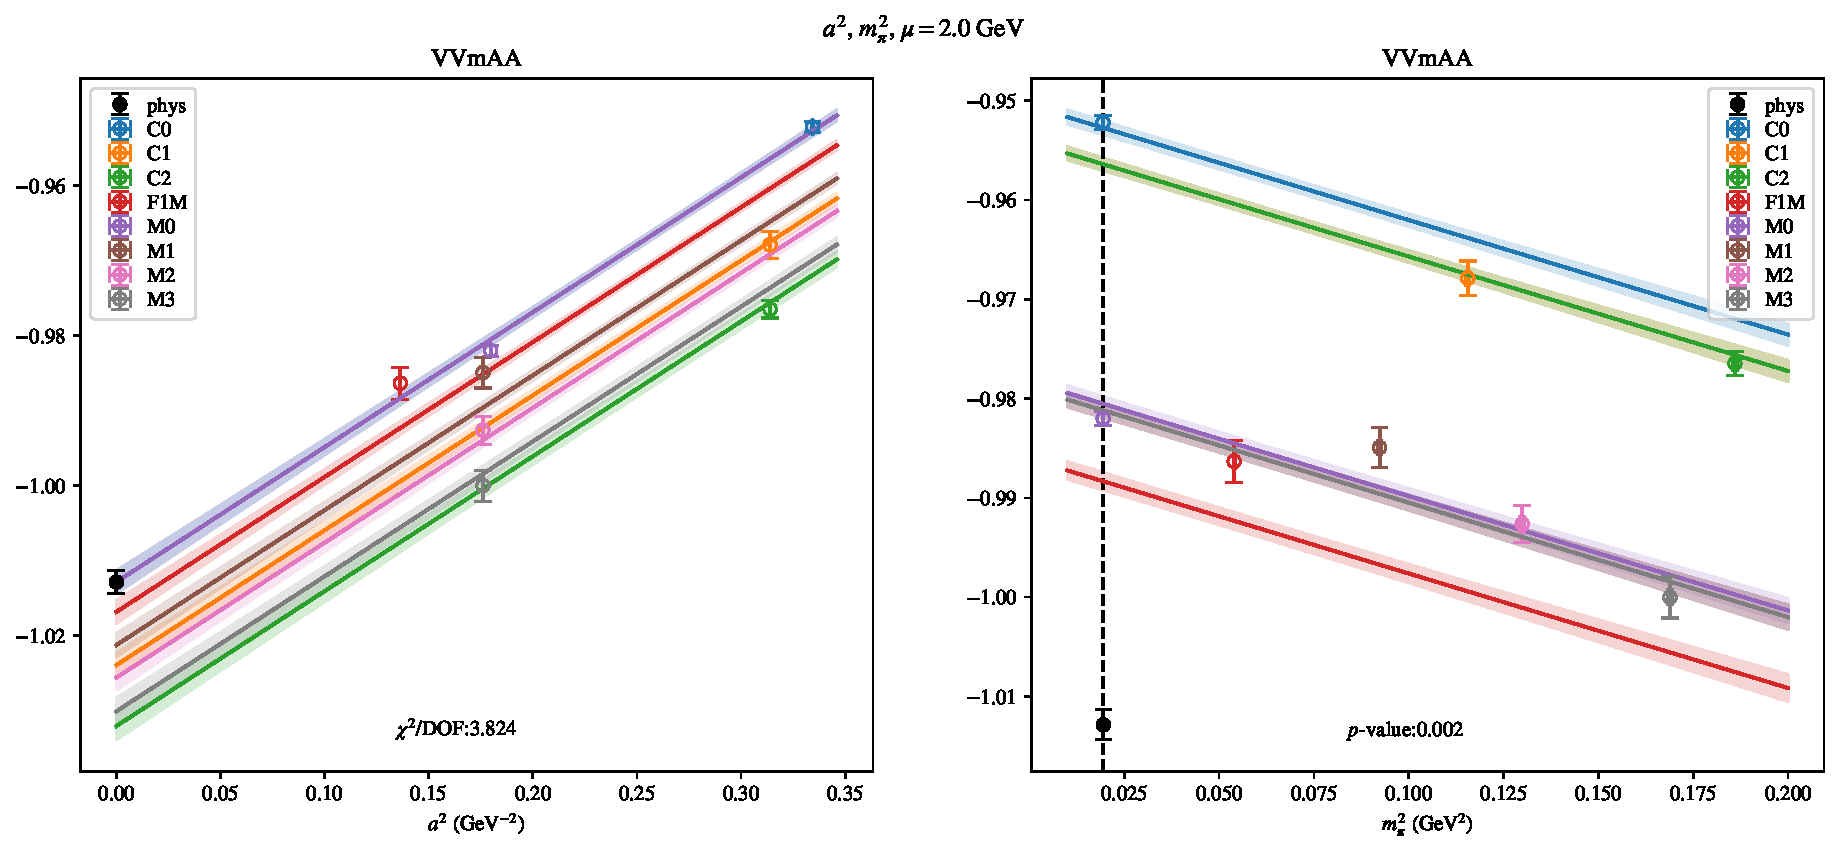
\includepdf[link, pages=-]{VVmAA/NPR/a2m2_20.pdf}
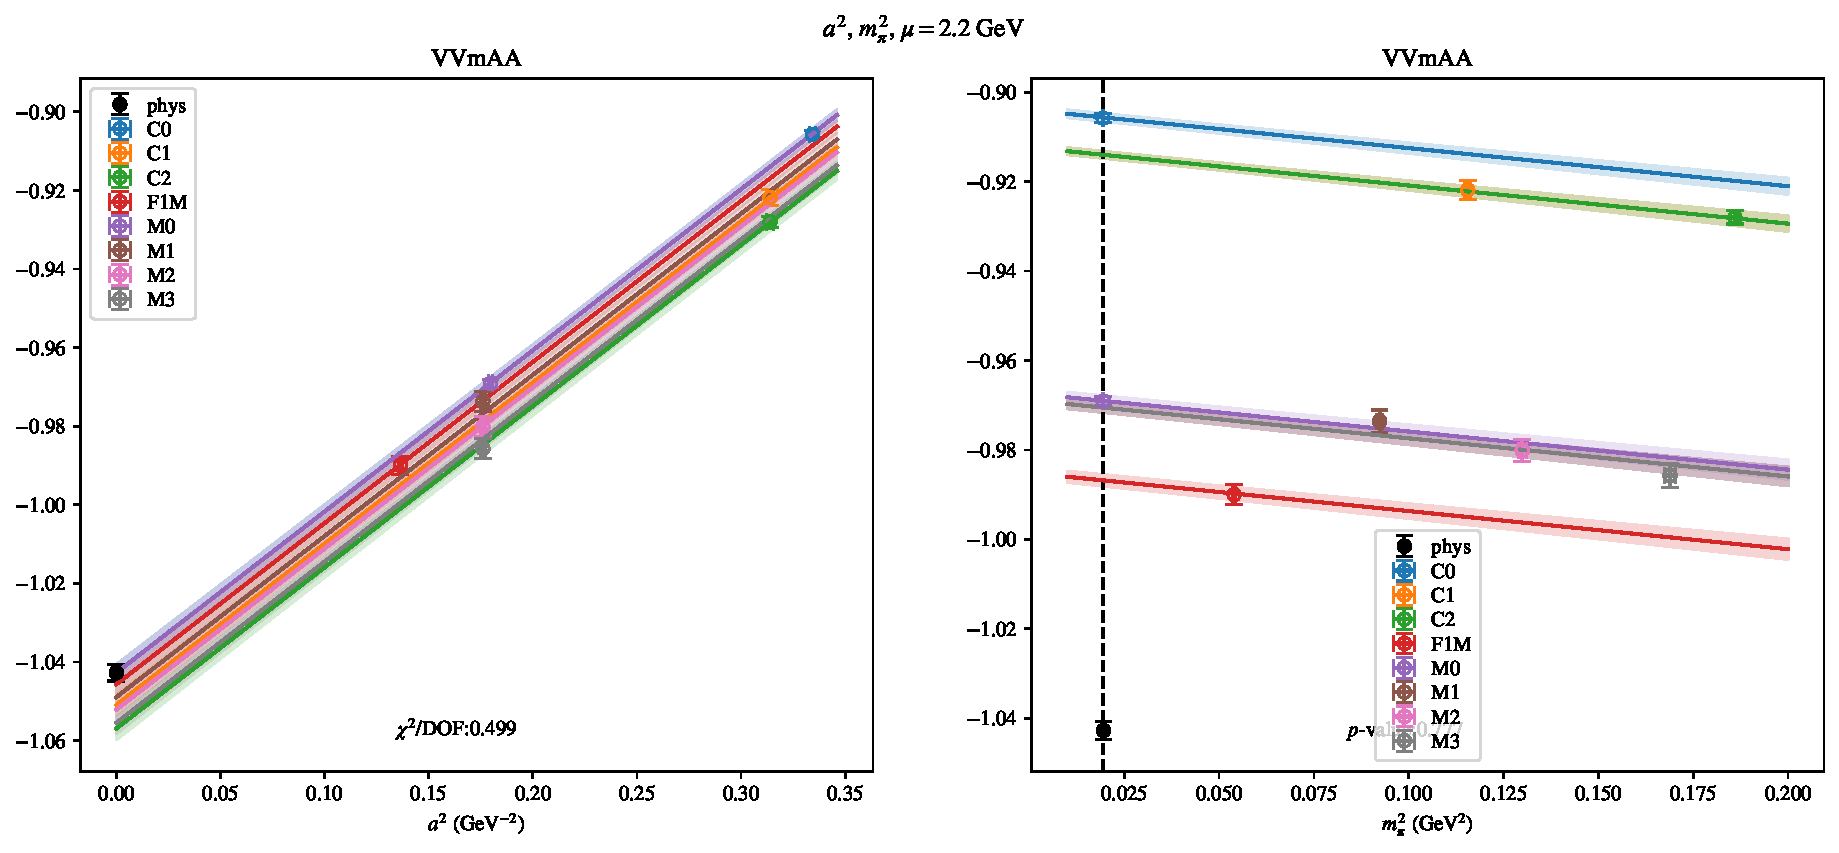
\includepdf[link, pages=-]{VVmAA/NPR/a2m2_22.pdf}
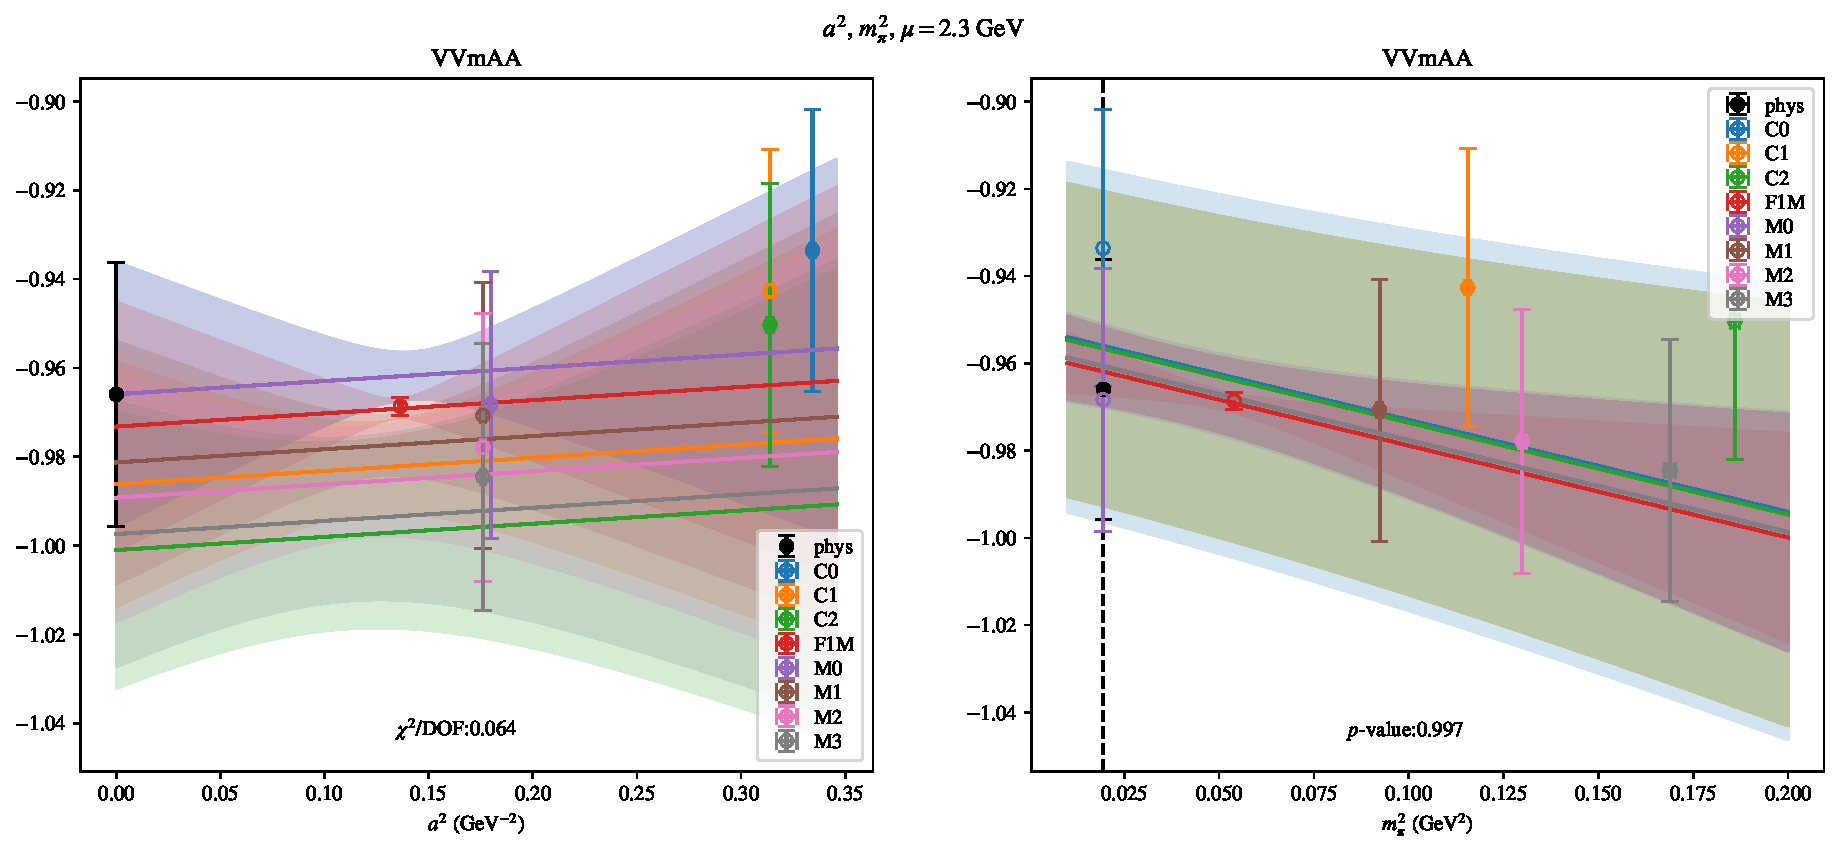
\includepdf[link, pages=-]{VVmAA/NPR/a2m2_23.pdf}
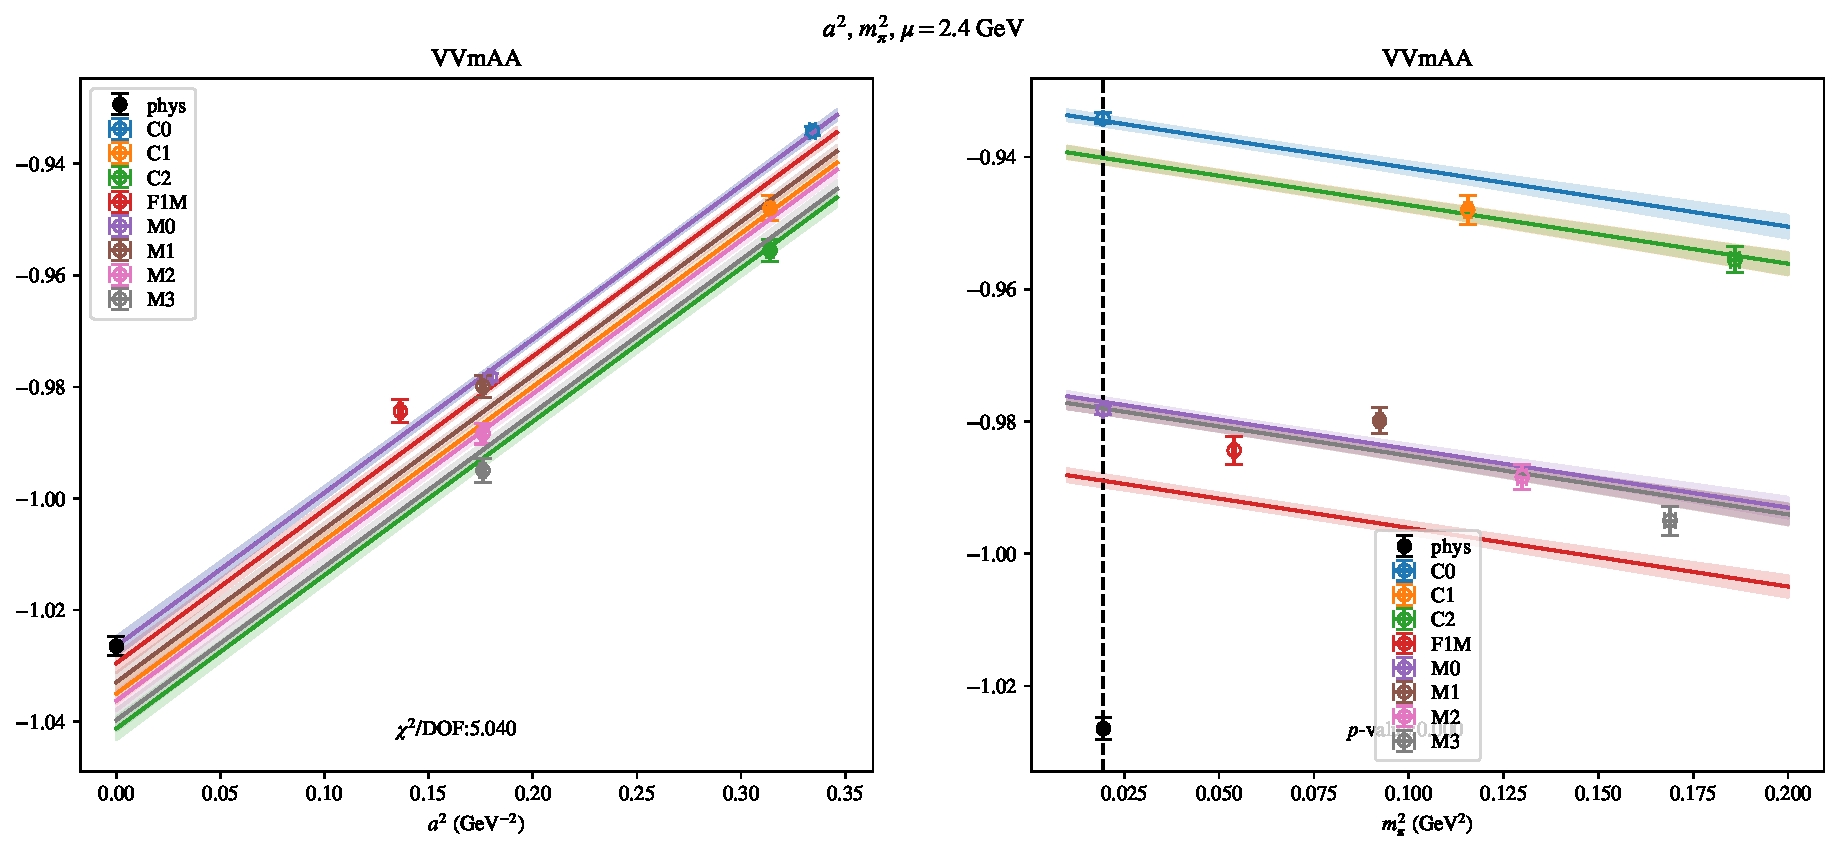
\includepdf[link, pages=-]{VVmAA/NPR/a2m2_24.pdf}
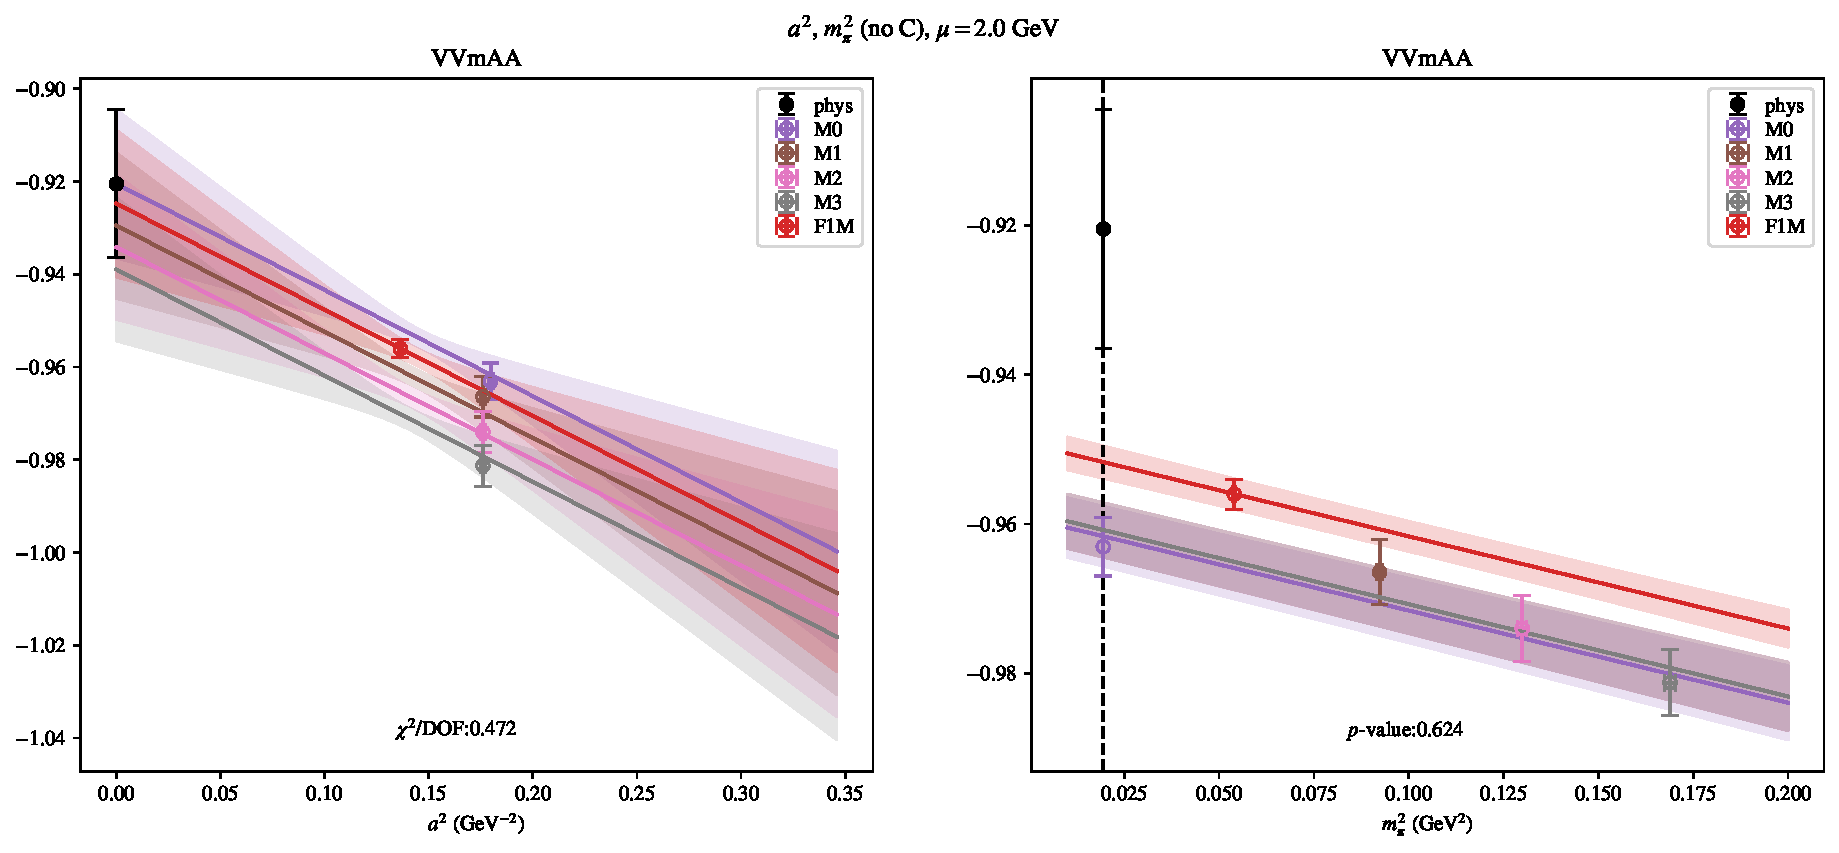
\includepdf[link, pages=-]{VVmAA/NPR/a2m2noC_20.pdf}
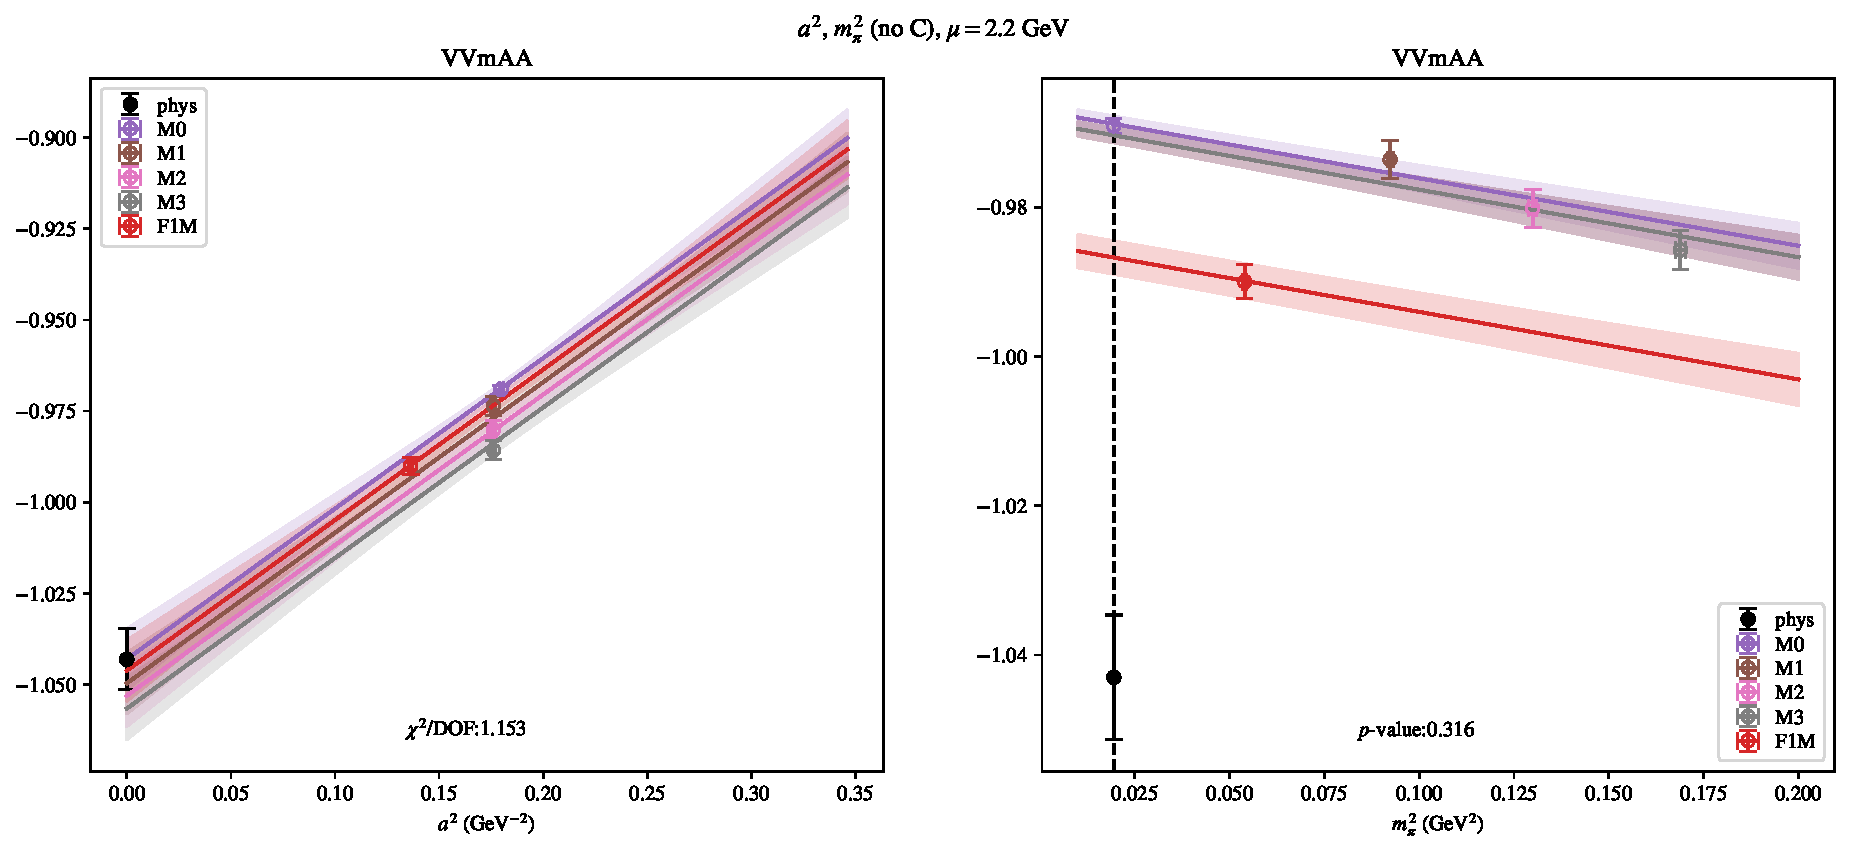
\includepdf[link, pages=-]{VVmAA/NPR/a2m2noC_22.pdf}
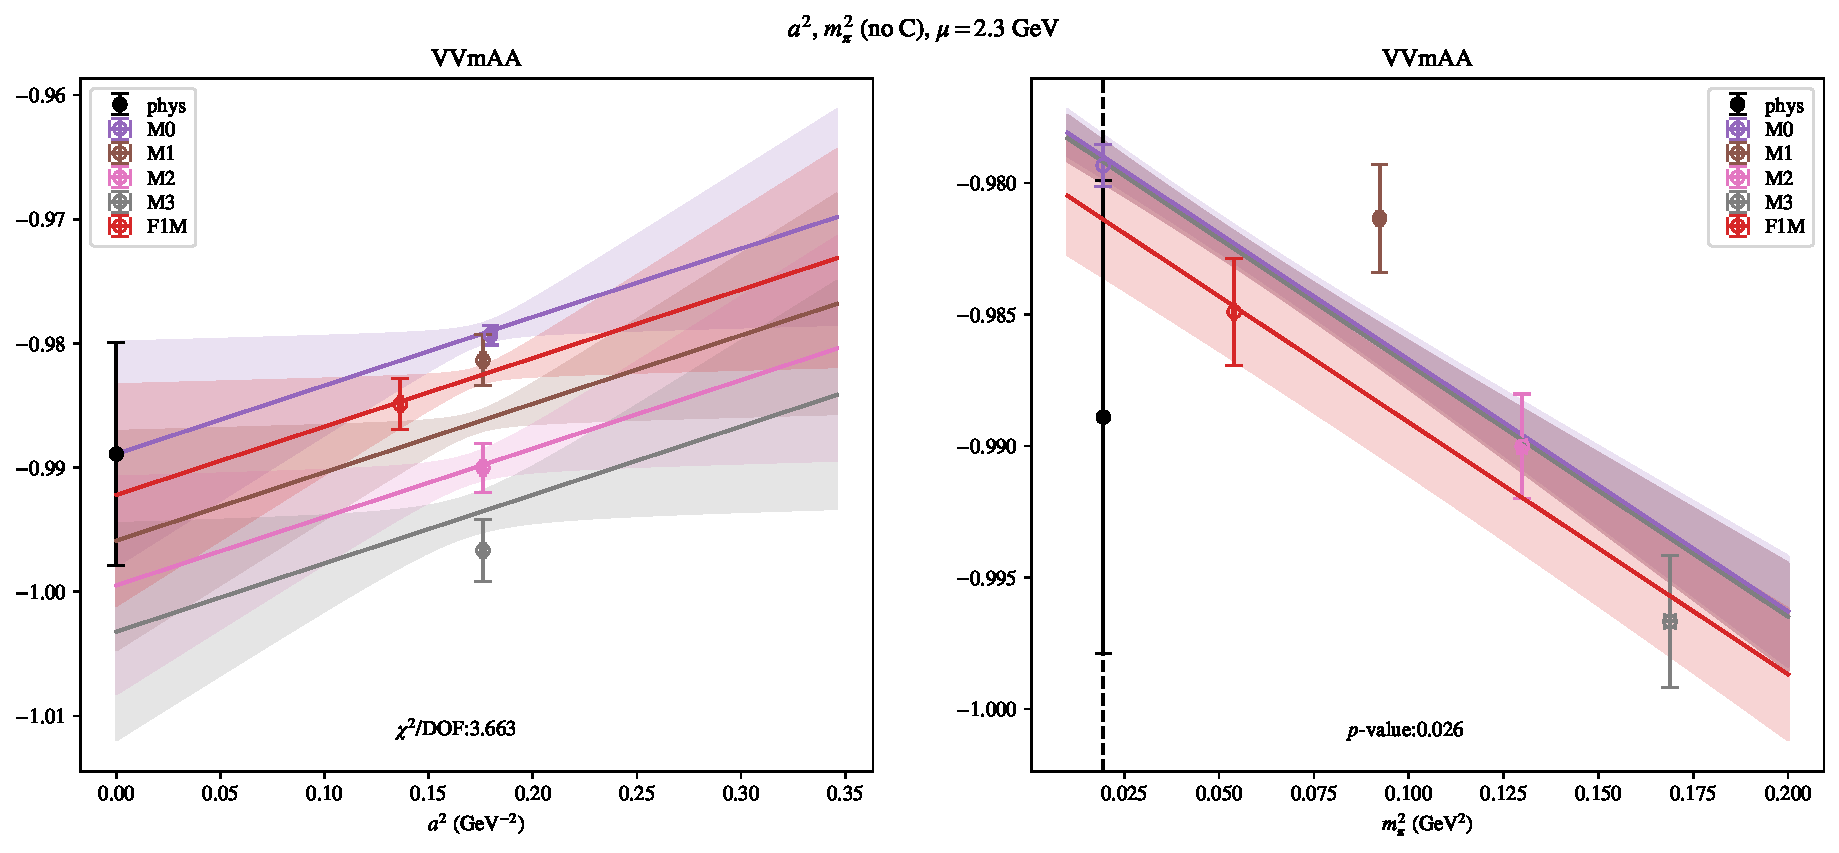
\includepdf[link, pages=-]{VVmAA/NPR/a2m2noC_23.pdf}
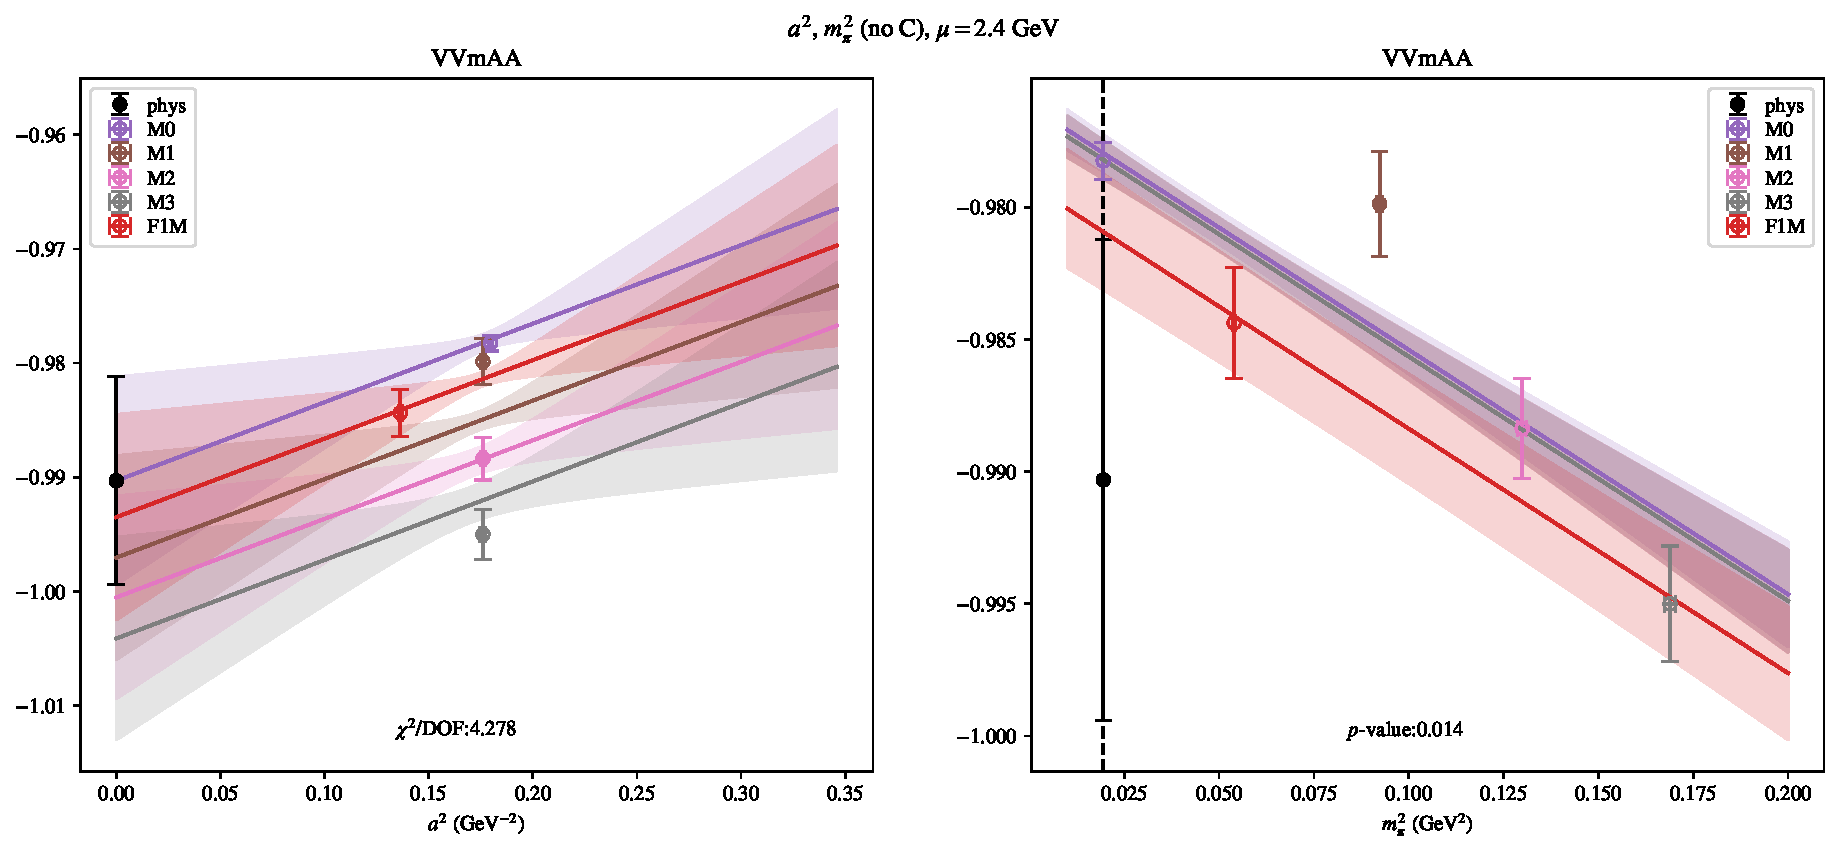
\includepdf[link, pages=-]{VVmAA/NPR/a2m2noC_24.pdf}
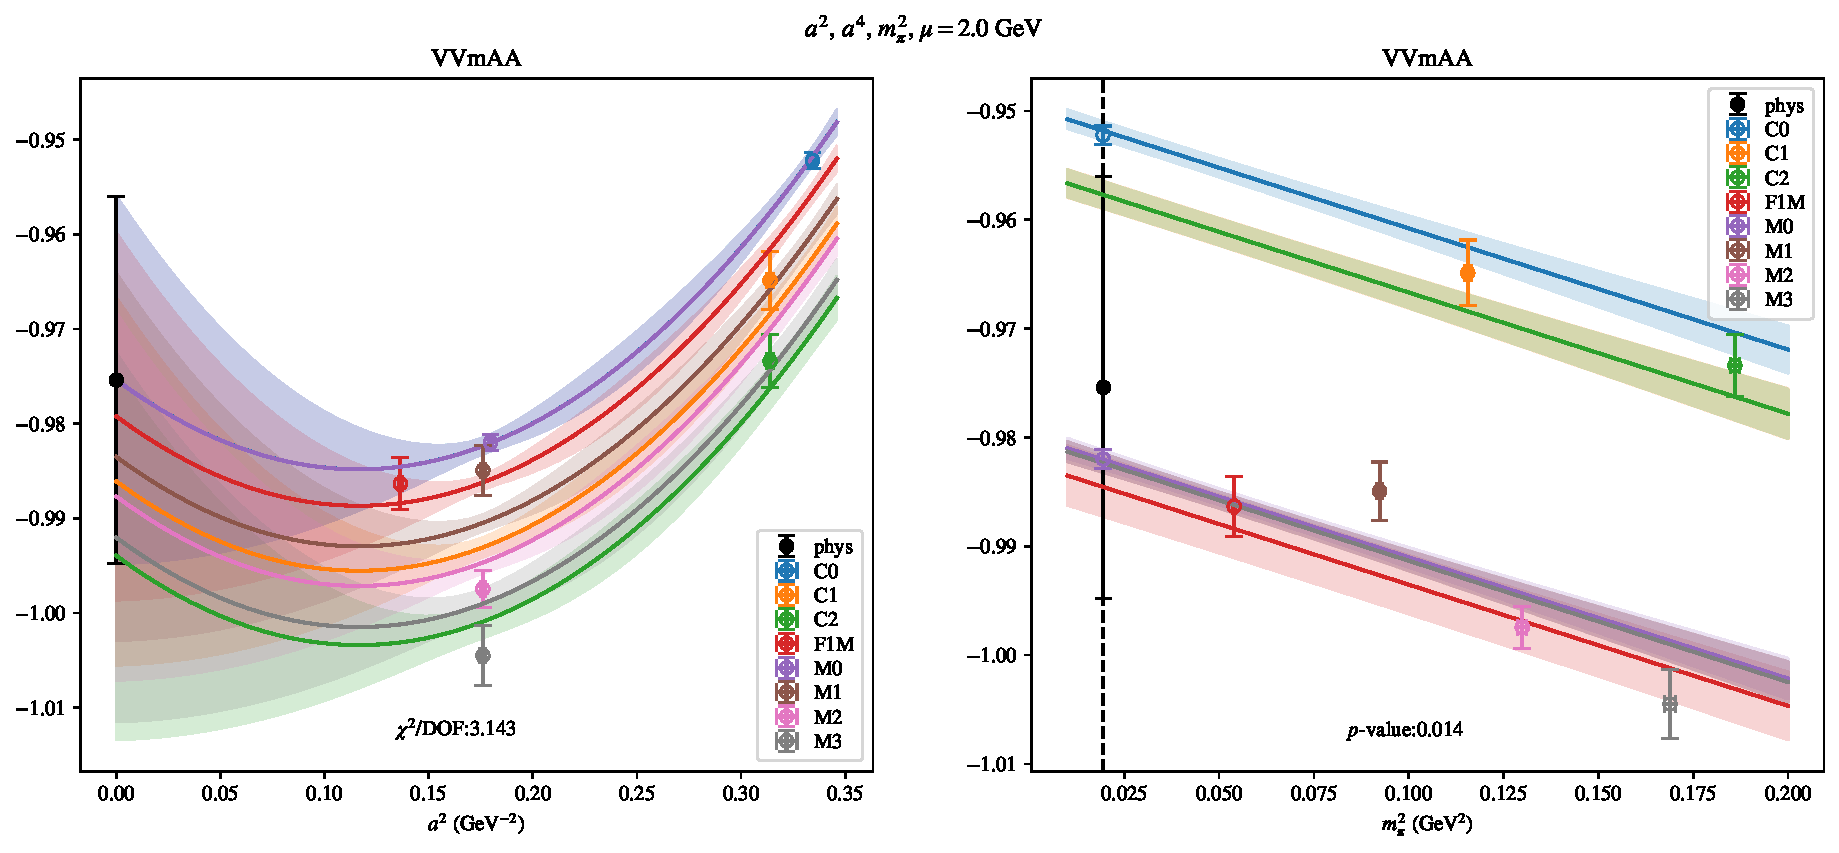
\includepdf[link, pages=-]{VVmAA/NPR/a2a4m2_20.pdf}
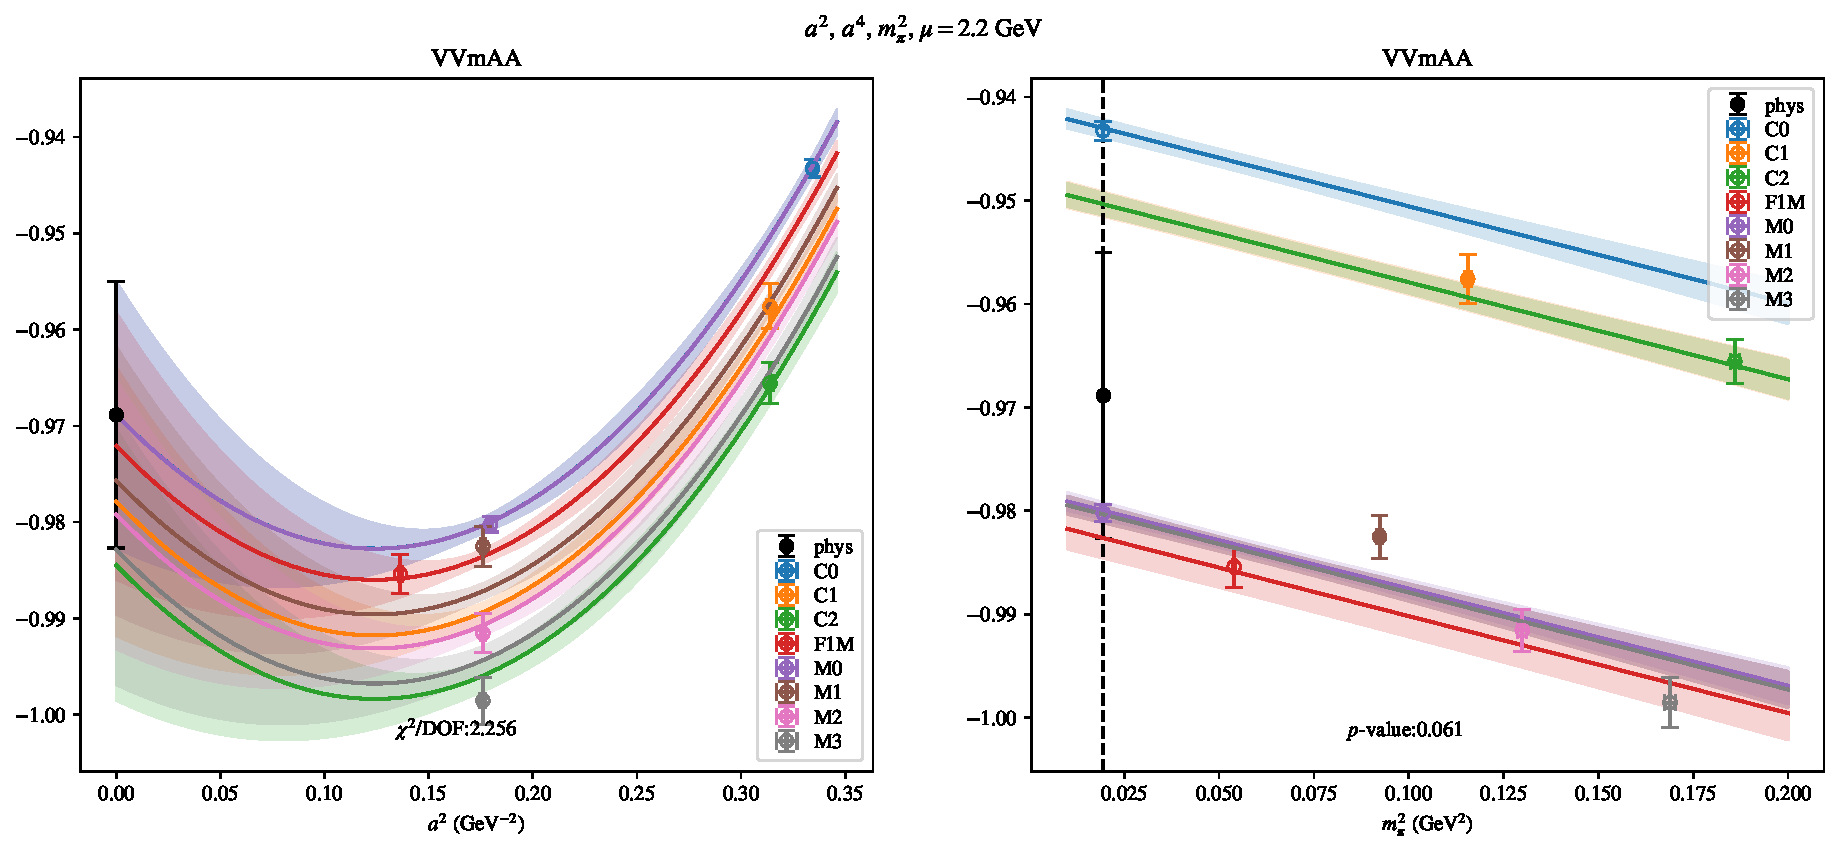
\includepdf[link, pages=-]{VVmAA/NPR/a2a4m2_22.pdf}
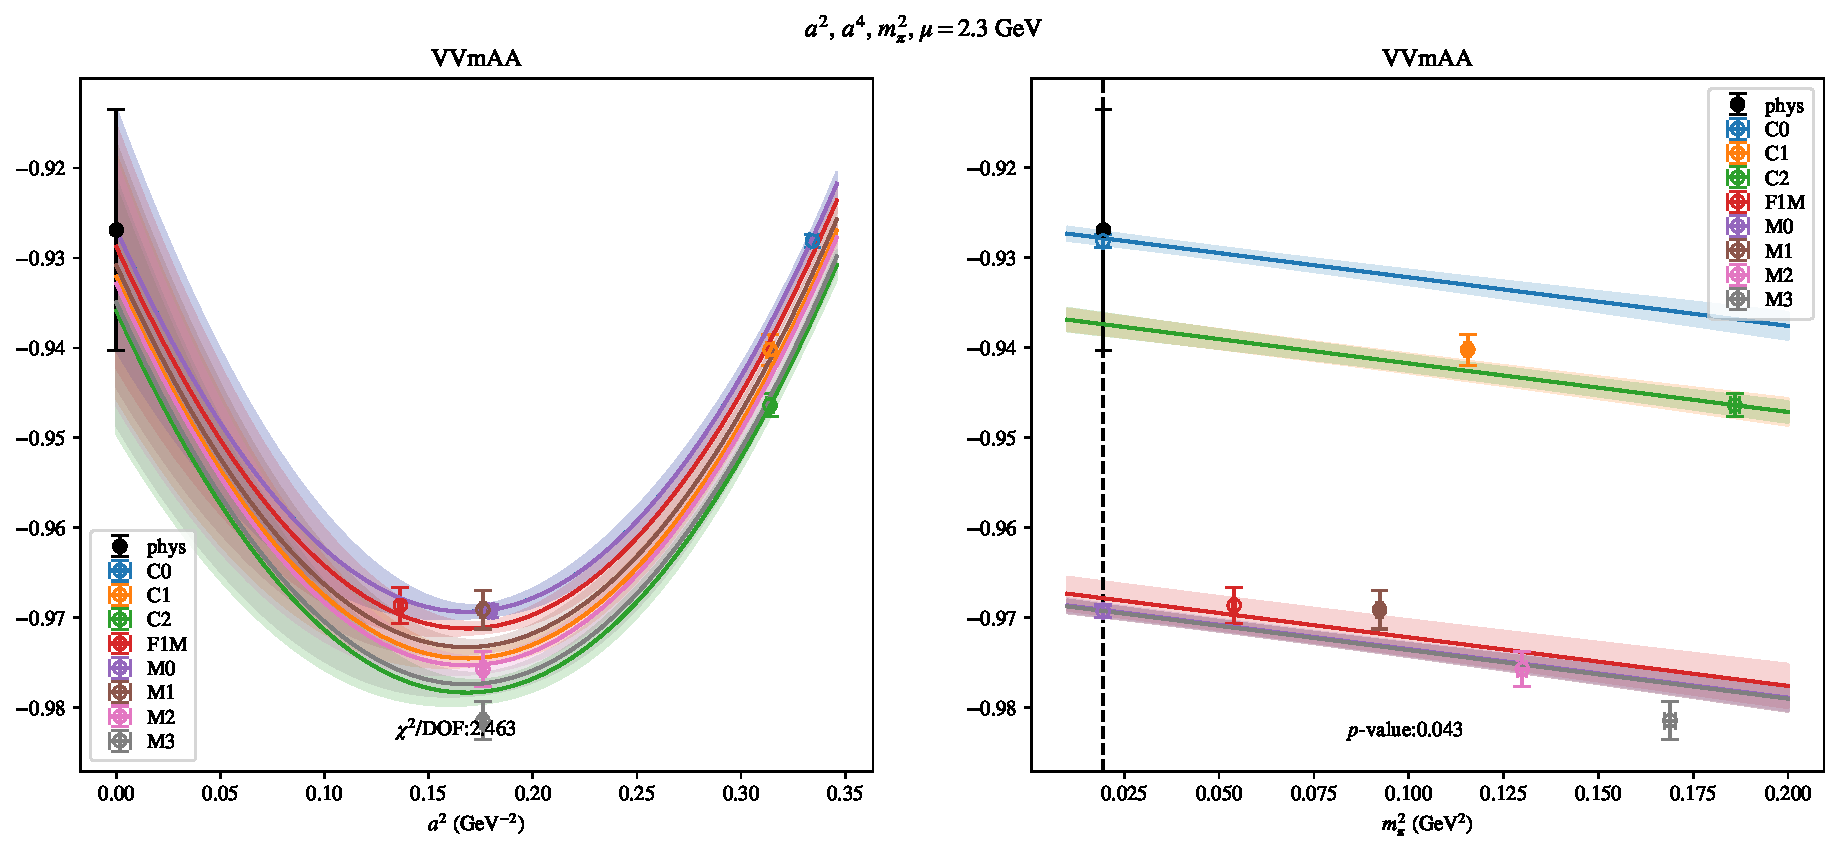
\includepdf[link, pages=-]{VVmAA/NPR/a2a4m2_23.pdf}
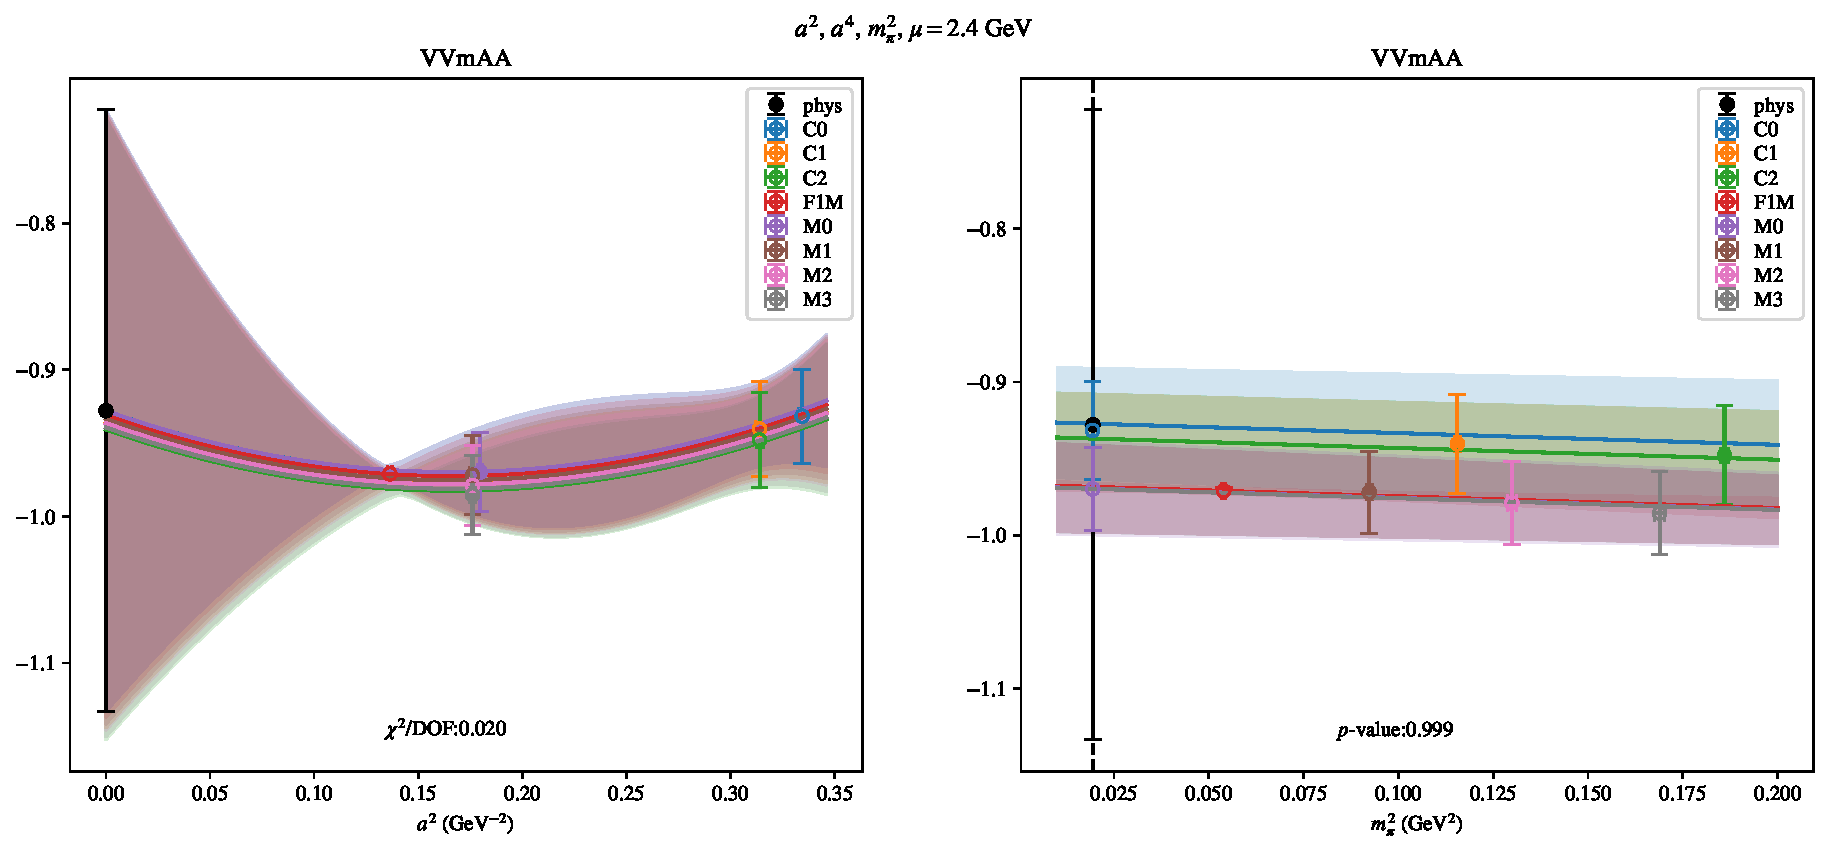
\includepdf[link, pages=-]{VVmAA/NPR/a2a4m2_24.pdf}
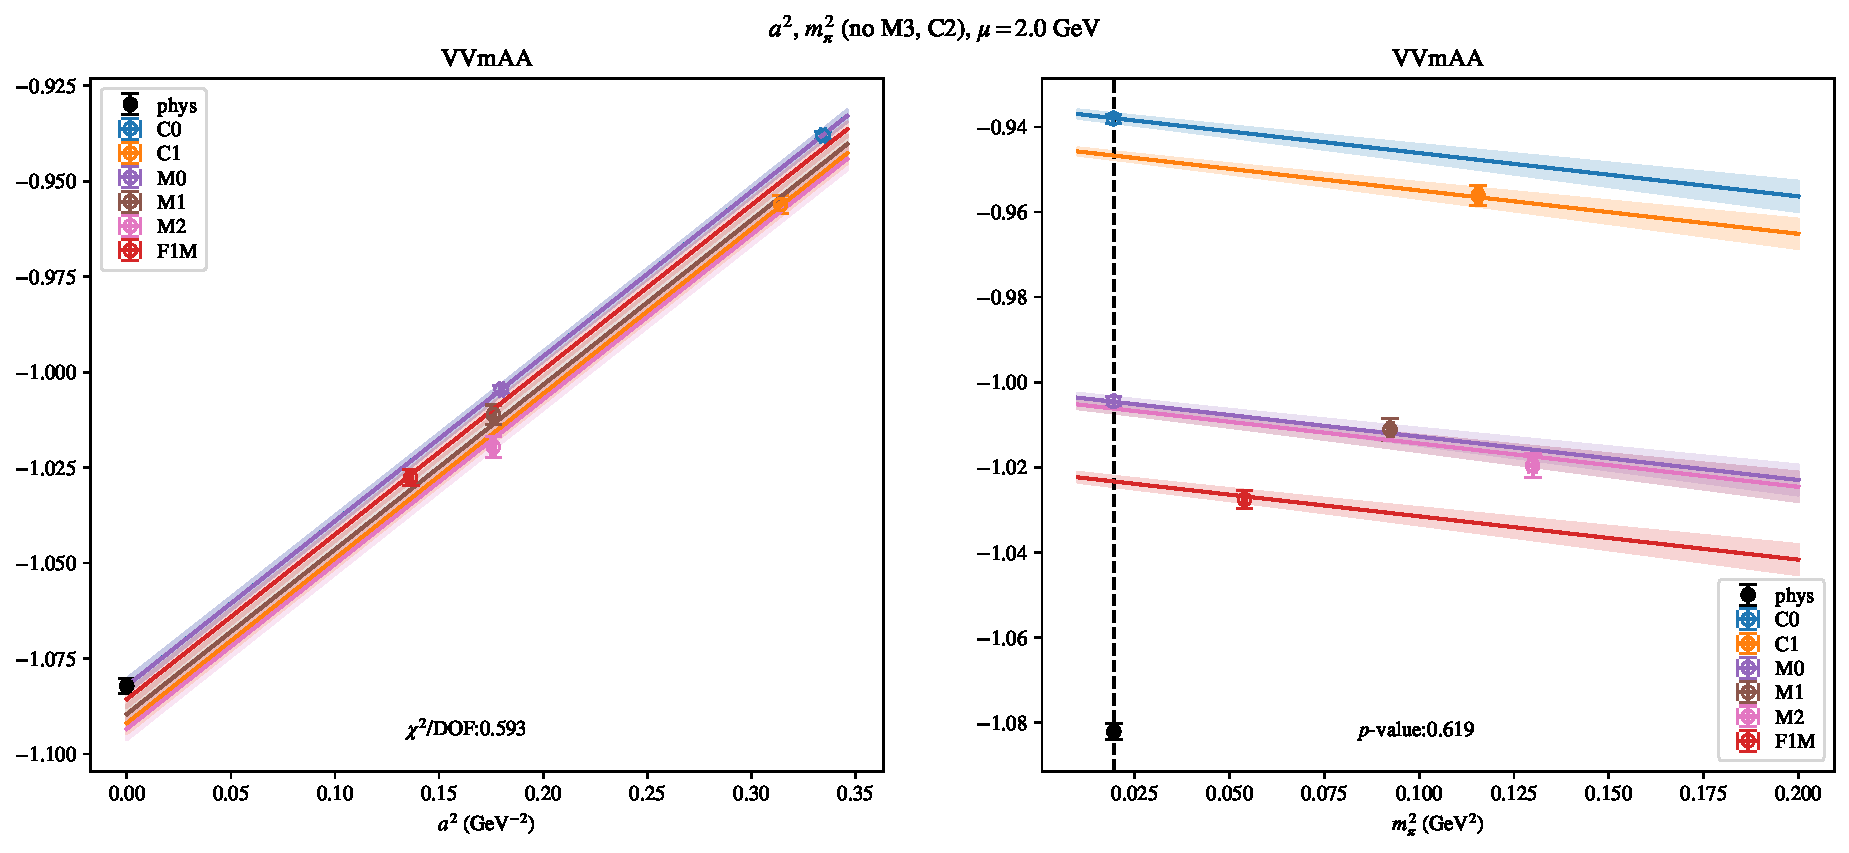
\includepdf[link, pages=-]{VVmAA/NPR/a2m2mcut_20.pdf}
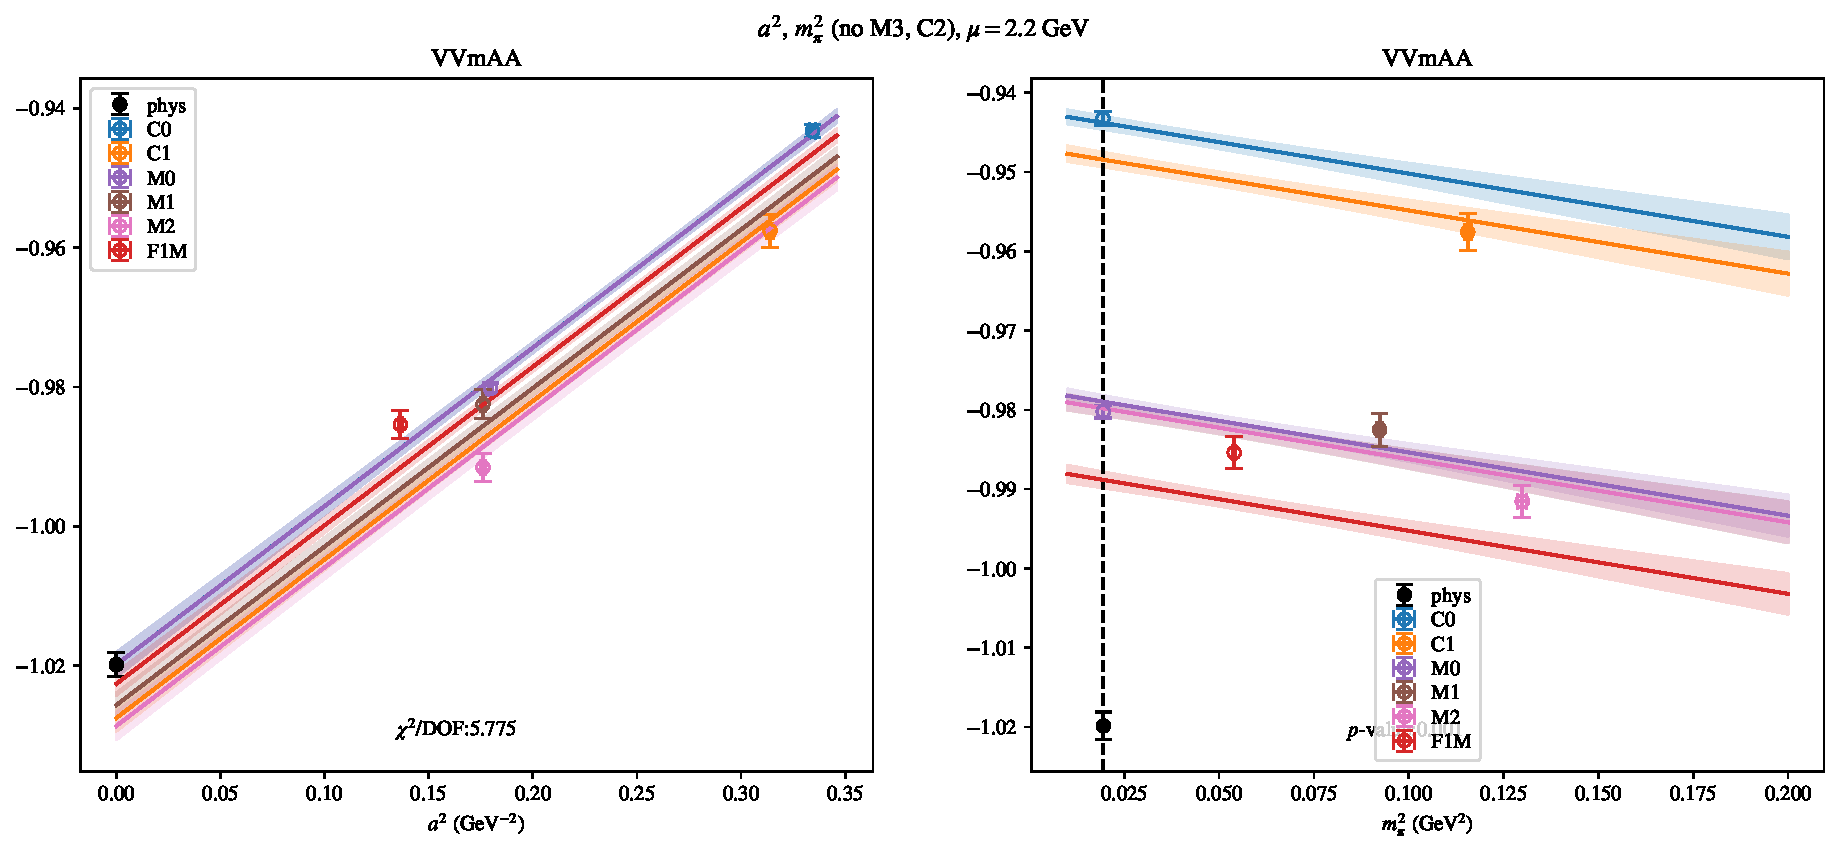
\includepdf[link, pages=-]{VVmAA/NPR/a2m2mcut_22.pdf}
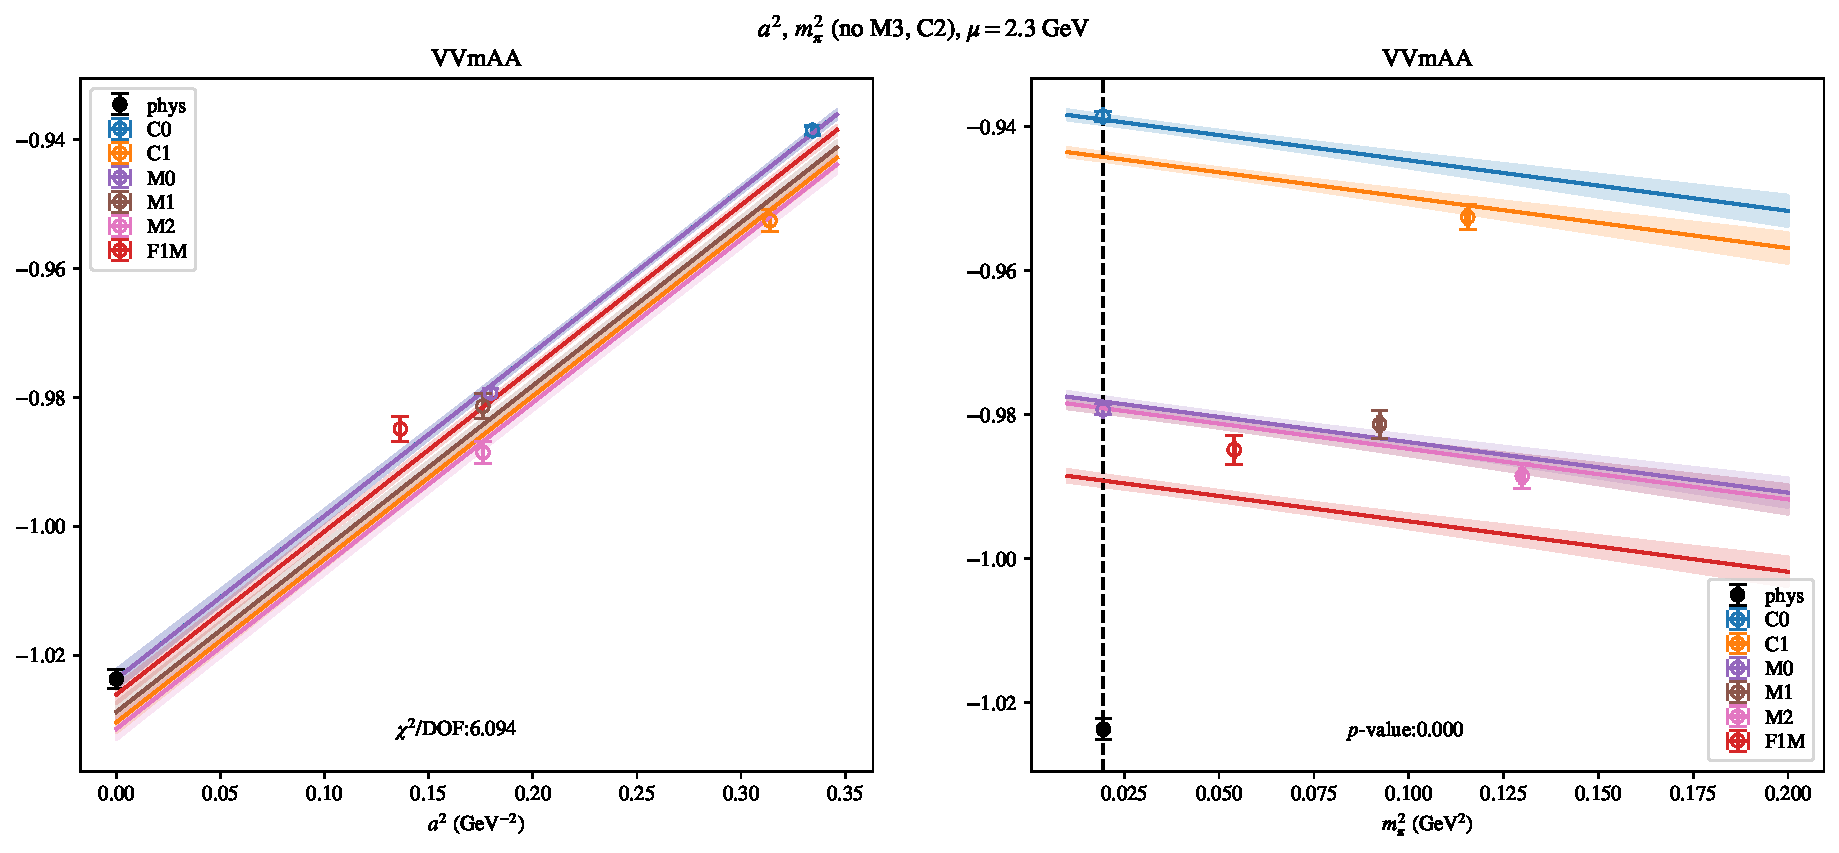
\includepdf[link, pages=-]{VVmAA/NPR/a2m2mcut_23.pdf}
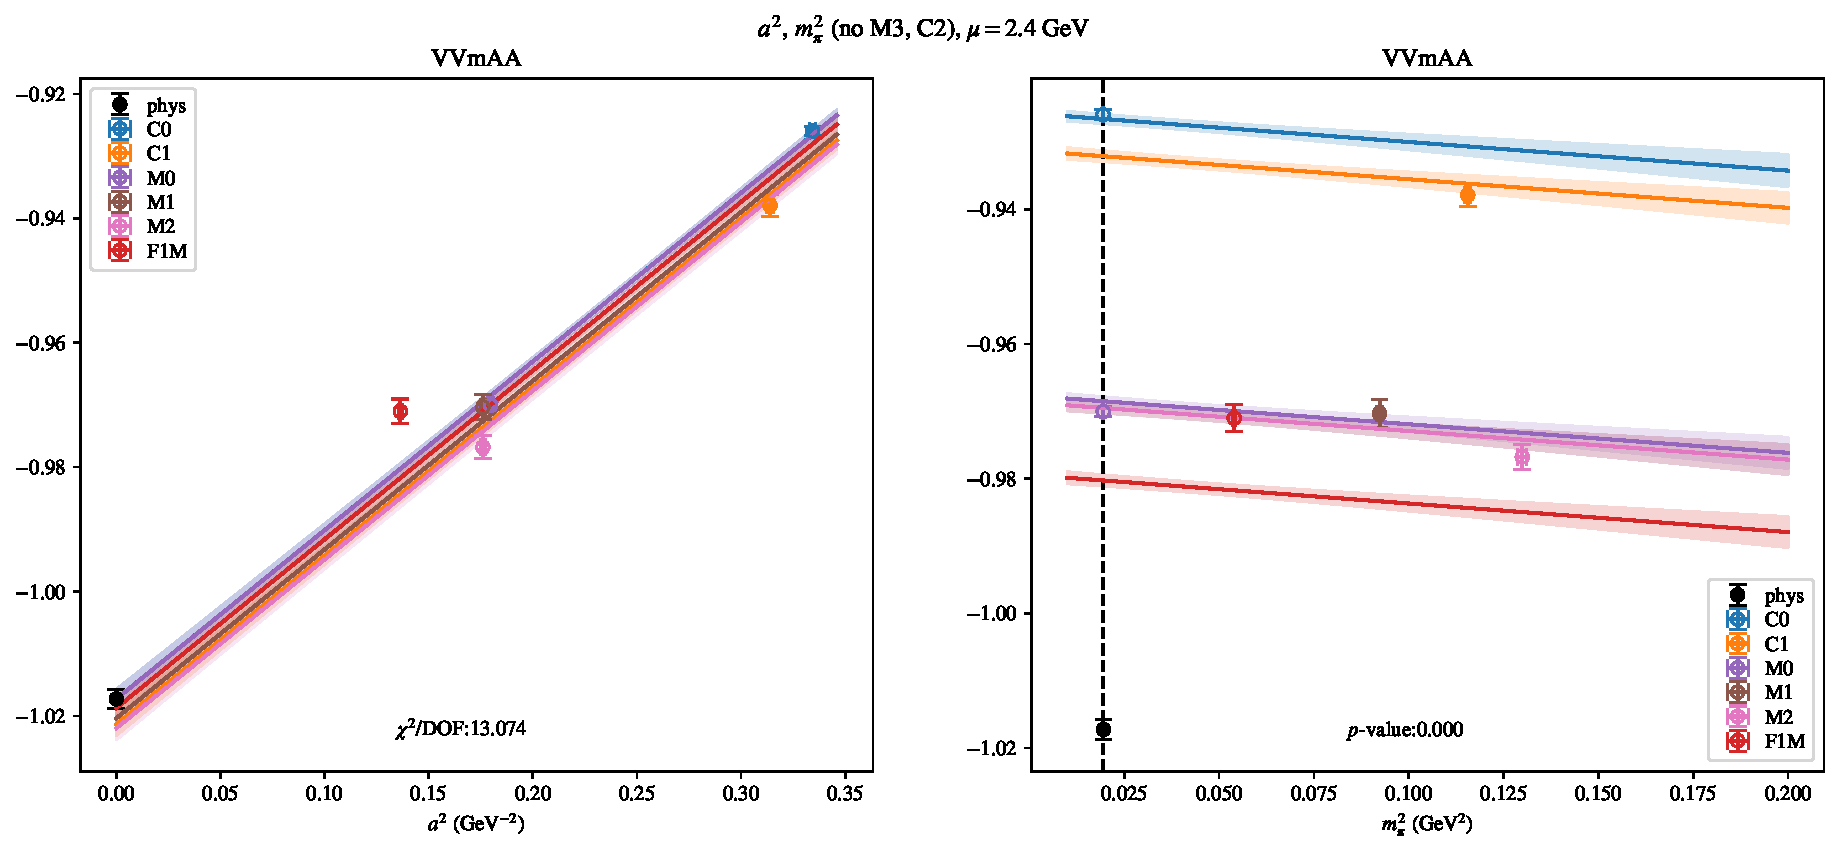
\includepdf[link, pages=-]{VVmAA/NPR/a2m2mcut_24.pdf}
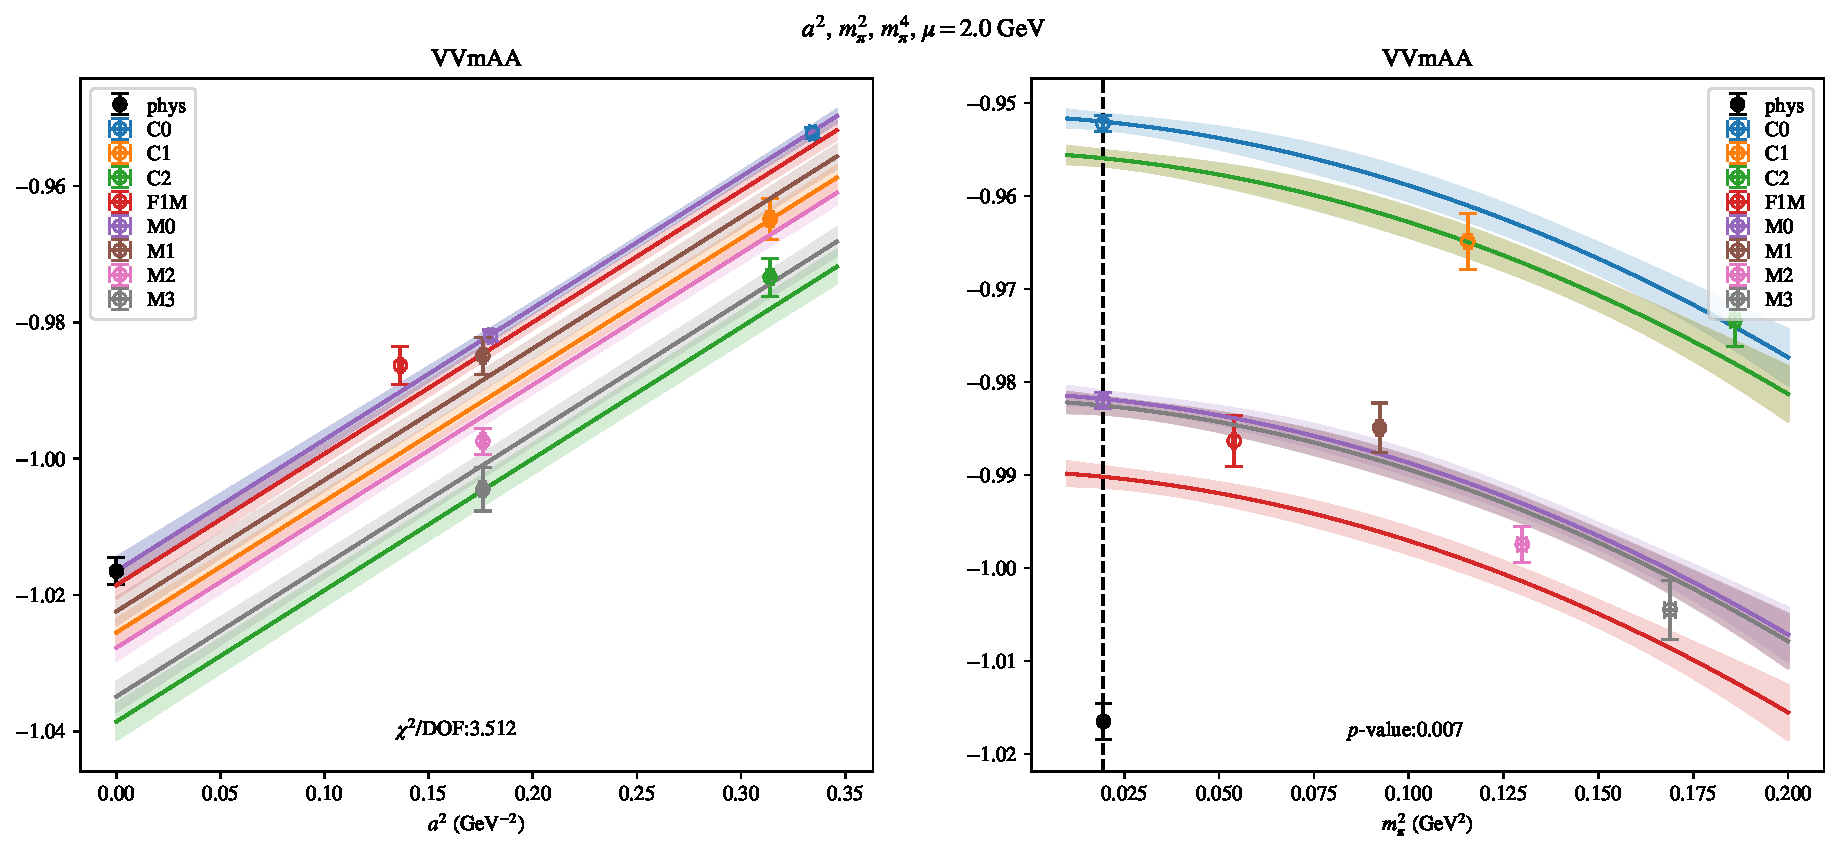
\includepdf[link, pages=-]{VVmAA/NPR/a2m2m4_20.pdf}
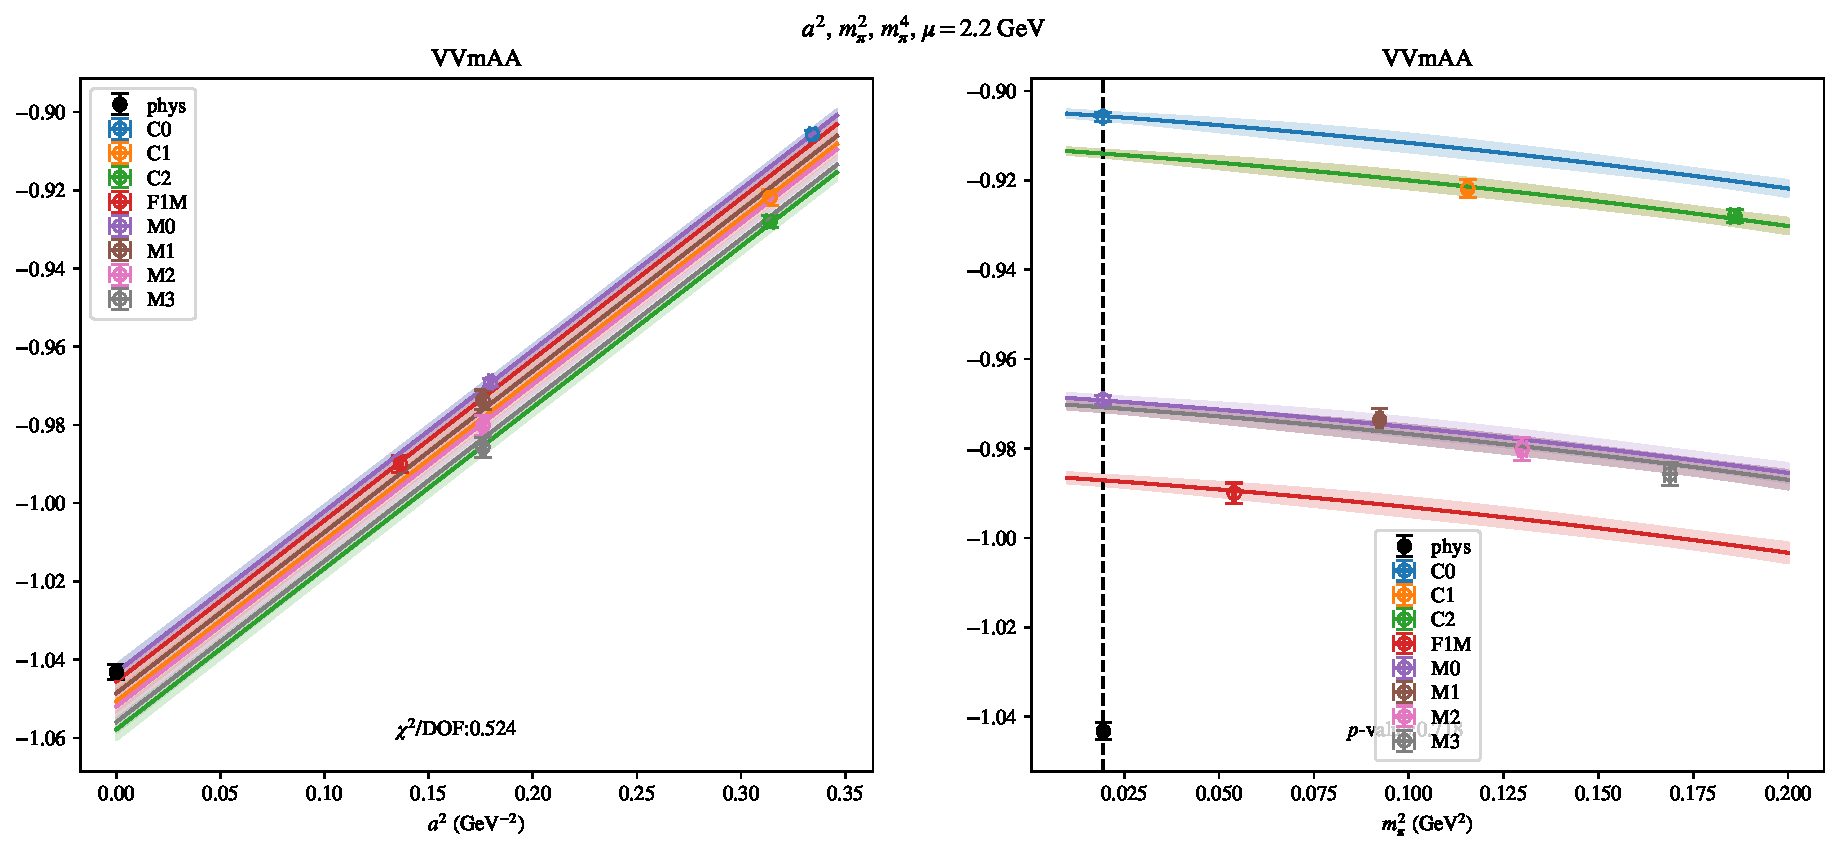
\includepdf[link, pages=-]{VVmAA/NPR/a2m2m4_22.pdf}
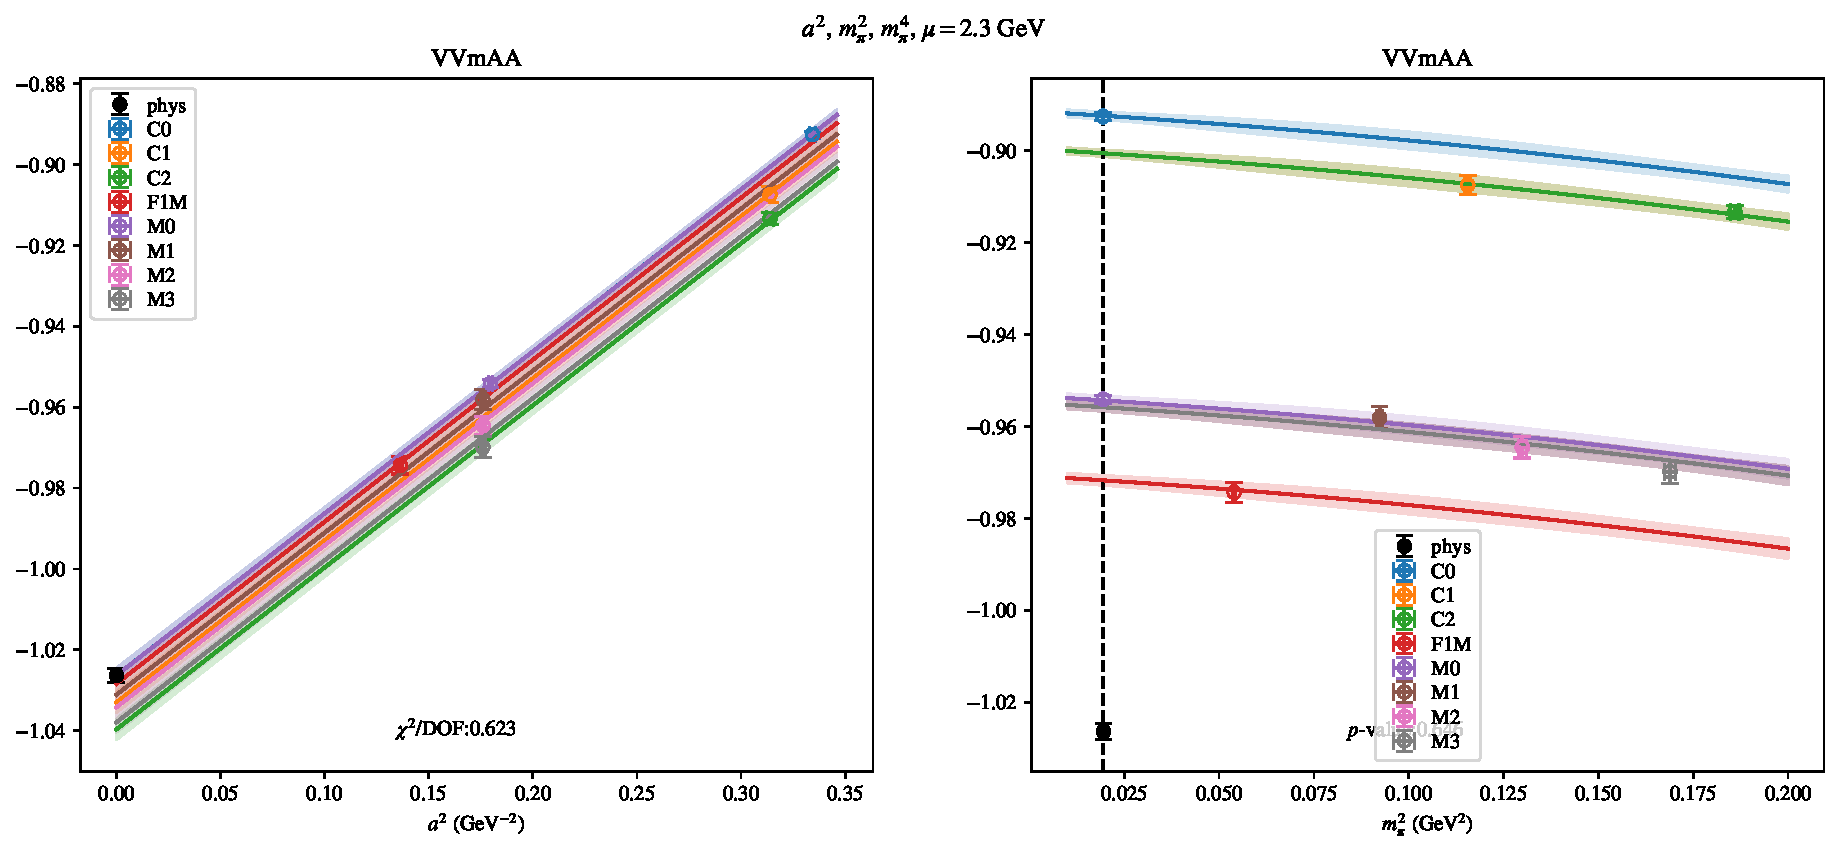
\includepdf[link, pages=-]{VVmAA/NPR/a2m2m4_23.pdf}
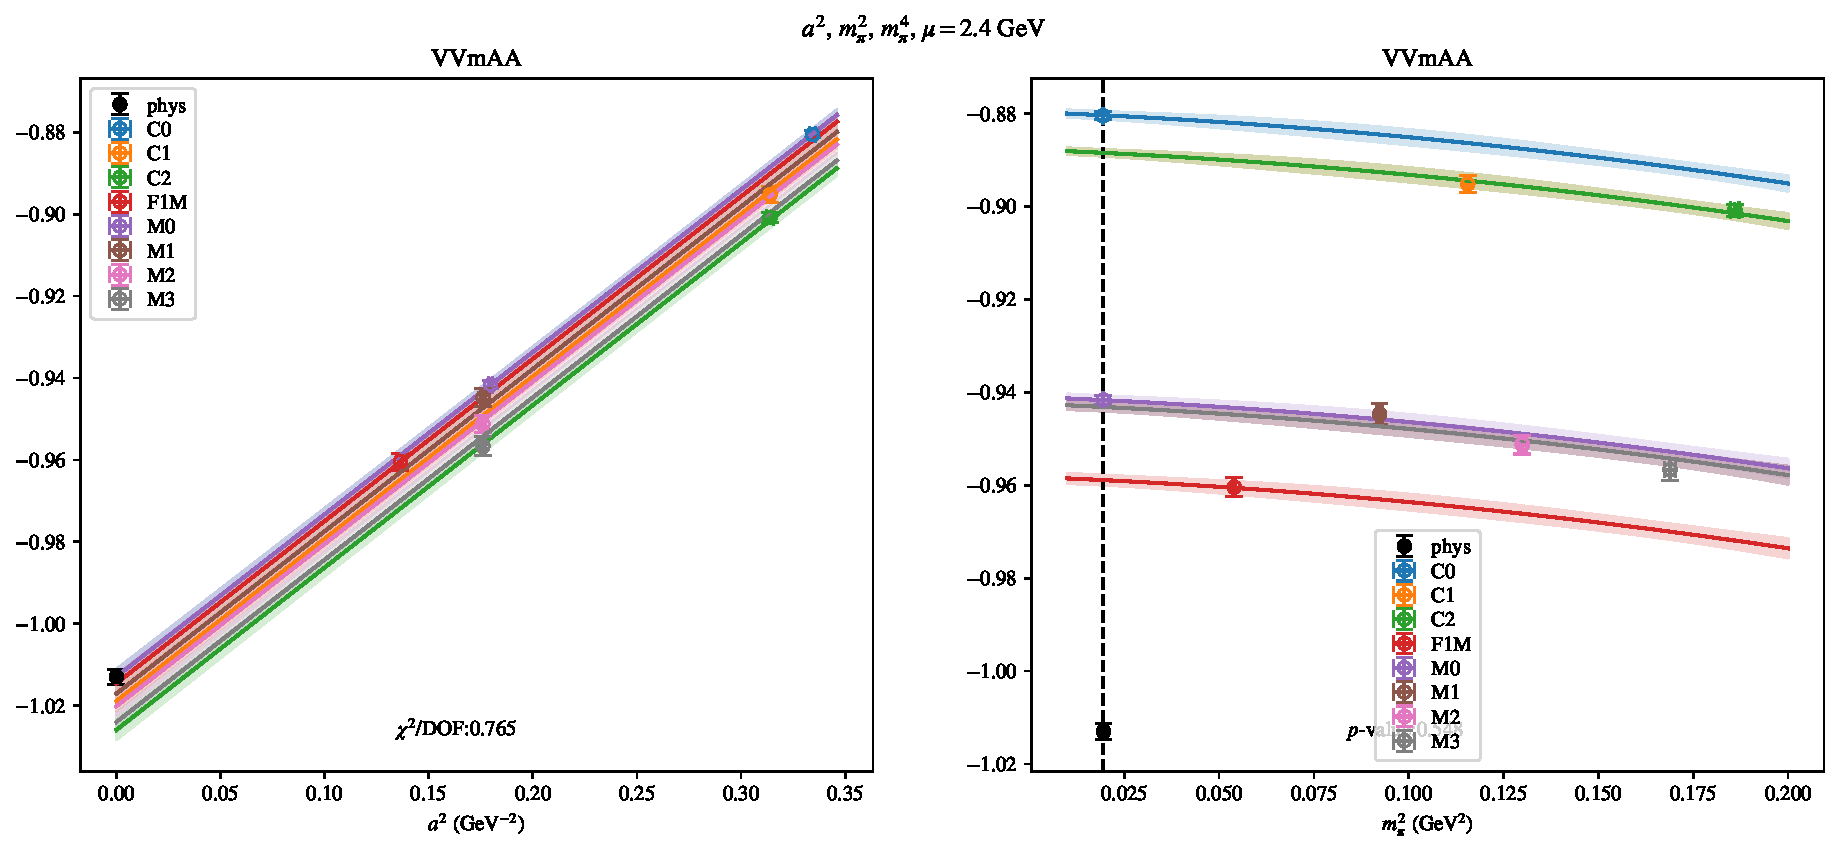
\includepdf[link, pages=-]{VVmAA/NPR/a2m2m4_24.pdf}
\clearpage
\section{$\mathcal{B}_3$}
\begin{table}[h!]
\begin{center}
\begin{tabular}{|c|c|c|c|c|c|}
\hline
$\mu$ (GeV) & $a^2$, $m_\pi^2$& $a^2$, $m_\pi^2$ (no C)& $a^2$, $a^4$, $m_\pi^2$& $a^2$, $m_\pi^2$ (no M3, C2)& $a^2$, $m_\pi^2$, $m_\pi^4$\\
\hline
2.0& \hyperlink{SSmPP/NPR/a2m2_20.pdf.1}{\textbf{1.7999(28)}: 15.728 (0.0)} & \hyperlink{SSmPP/NPR/a2m2noC_20.pdf.1}{\textbf{1.692(13)}: 0.635 (0.53)} & \hyperlink{SSmPP/NPR/a2a4m2_20.pdf.1}{\textbf{1.622(21)}: 1.018 (0.396)} & \hyperlink{SSmPP/NPR/a2m2mcut_20.pdf.1}{\textbf{1.8011(28)}: 24.84 (0.0)} & \hyperlink{SSmPP/NPR/a2m2m4_20.pdf.1}{\textbf{1.8049(29)}: 15.268 (0.0)}\\
2.2& \hyperlink{SSmPP/NPR/a2m2_22.pdf.1}{\textbf{1.8055(26)}: 14.624 (0.0)} & \hyperlink{SSmPP/NPR/a2m2noC_22.pdf.1}{\textbf{1.705(13)}: 1.349 (0.26)} & \hyperlink{SSmPP/NPR/a2a4m2_22.pdf.1}{\textbf{1.639(21)}: 1.498 (0.2)} & \hyperlink{SSmPP/NPR/a2m2mcut_22.pdf.1}{\textbf{1.8069(28)}: 22.011 (0.0)} & \hyperlink{SSmPP/NPR/a2m2m4_22.pdf.1}{\textbf{1.8106(28)}: 13.322 (0.0)}\\
2.3& \hyperlink{SSmPP/NPR/a2m2_23.pdf.1}{\textbf{1.8079(26)}: 14.078 (0.0)} & \hyperlink{SSmPP/NPR/a2m2noC_23.pdf.1}{\textbf{1.709(13)}: 1.503 (0.223)} & \hyperlink{SSmPP/NPR/a2a4m2_23.pdf.1}{\textbf{1.645(21)}: 1.393 (0.233)} & \hyperlink{SSmPP/NPR/a2m2mcut_23.pdf.1}{\textbf{1.8092(27)}: 21.405 (0.0)} & \hyperlink{SSmPP/NPR/a2m2m4_23.pdf.1}{\textbf{1.8128(27)}: 13.146 (0.0)}\\
2.4& \hyperlink{SSmPP/NPR/a2m2_24.pdf.1}{\textbf{1.8093(25)}: 13.05 (0.0)} & \hyperlink{SSmPP/NPR/a2m2noC_24.pdf.1}{\textbf{1.714(13)}: 1.501 (0.223)} & \hyperlink{SSmPP/NPR/a2a4m2_24.pdf.1}{\textbf{1.652(21)}: 1.372 (0.241)} & \hyperlink{SSmPP/NPR/a2m2mcut_24.pdf.1}{\textbf{1.8105(28)}: 19.973 (0.0)} & \hyperlink{SSmPP/NPR/a2m2m4_24.pdf.1}{\textbf{1.8141(27)}: 12.388 (0.0)}\\
\hline
\end{tabular}
\caption{Physical point value from chiral and continuum extrapolation at renormalisation scale $\mu$. Entries are \textbf{value(error)}: $\chi^2/\text{DOF}$ ($p$-value).}
\end{center}
\end{table}
\begin{table}[h!]
\begin{center}
\begin{tabular}{|c c|c|c|c|c|c|}
\hline
$\mu$ (GeV) &  & $a^2$, $m_\pi^2$& $a^2$, $m_\pi^2$ (no C)& $a^2$, $a^4$, $m_\pi^2$& $a^2$, $m_\pi^2$ (no M3, C2)& $a^2$, $m_\pi^2$, $m_\pi^4$\\
\hline
\multirow{2}{0.5in}{2.0} & $\alpha$ & 0.0707(59)& 0.446(49)& 1.06(13)& 0.0688(61)& 0.0615(62)\\
 & $\beta$ & -0.0010(13)& -0.0011(26)& -0.0015(16)& -0.0014(24)& -0.0040(71)\\
\hline
\multirow{2}{0.5in}{2.2} & $\alpha$ & 0.0763(56)& 0.425(47)& 0.99(13)& 0.0743(59)& 0.0671(58)\\
 & $\beta$ & -0.0007(12)& -0.0008(24)& -0.0011(15)& -0.0012(22)& -0.0036(66)\\
\hline
\multirow{2}{0.5in}{2.3} & $\alpha$ & 0.0773(55)& 0.417(47)& 0.97(13)& 0.0755(58)& 0.0684(58)\\
 & $\beta$ & -0.0007(11)& -0.0008(23)& -0.0011(14)& -0.0011(22)& -0.0034(64)\\
\hline
\multirow{2}{0.5in}{2.4} & $\alpha$ & 0.0792(54)& 0.406(46)& 0.93(12)& 0.0774(58)& 0.0704(58)\\
 & $\beta$ & -0.0006(11)& -0.0007(22)& -0.0010(14)& -0.0010(21)& -0.0031(63)\\
\hline
\end{tabular}
\caption{Fit values of coefficients in $Q = Q_{phys} + \mathbf{\alpha} a^2 + \mathbf{\beta}\left(\frac{m_\pi^2}{f_\pi^2}-\frac{m_{\pi,PDG}^2}{f_\pi^2}\right) + \ldots$.}
\end{center}
\end{table}
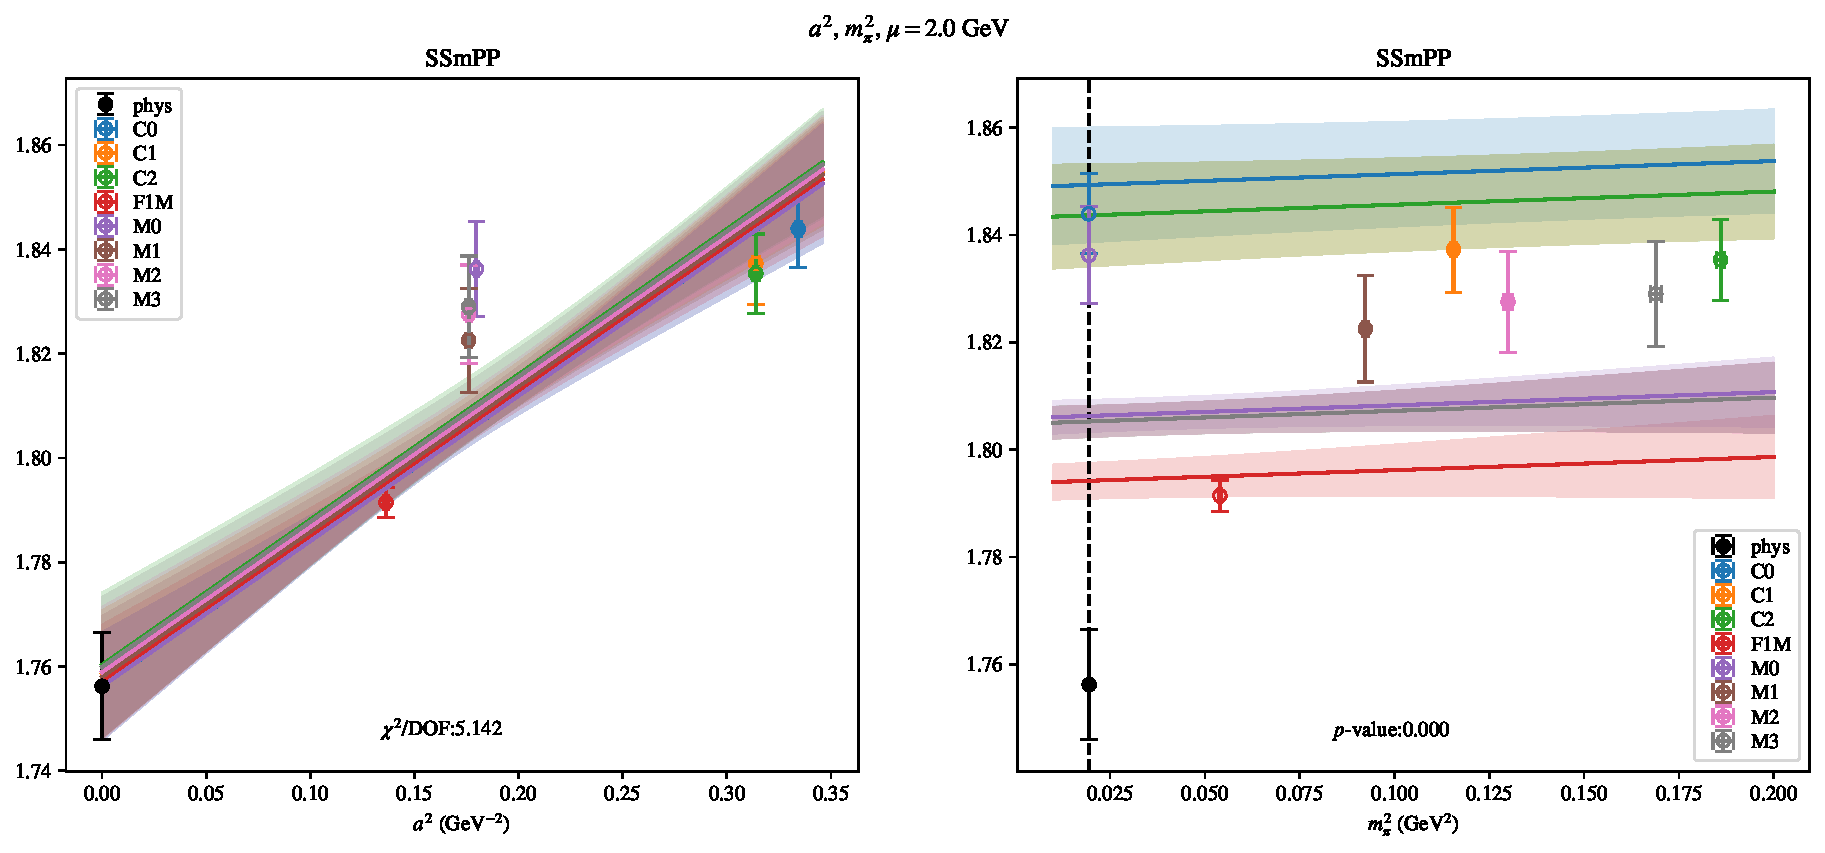
\includepdf[link, pages=-]{SSmPP/NPR/a2m2_20.pdf}
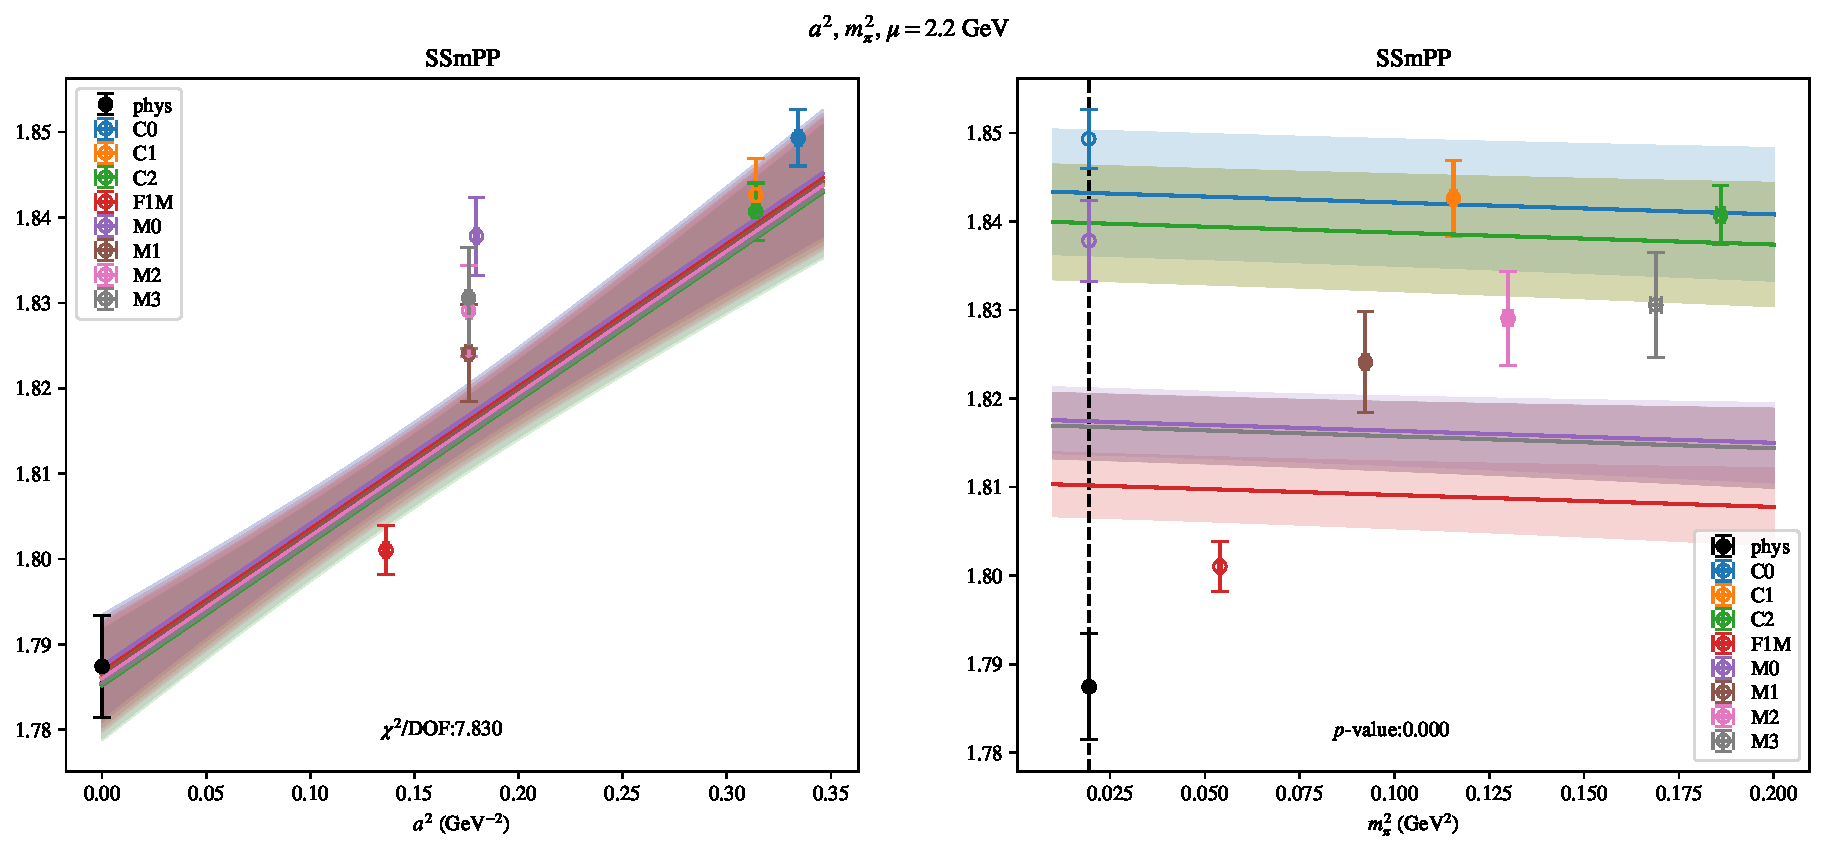
\includepdf[link, pages=-]{SSmPP/NPR/a2m2_22.pdf}
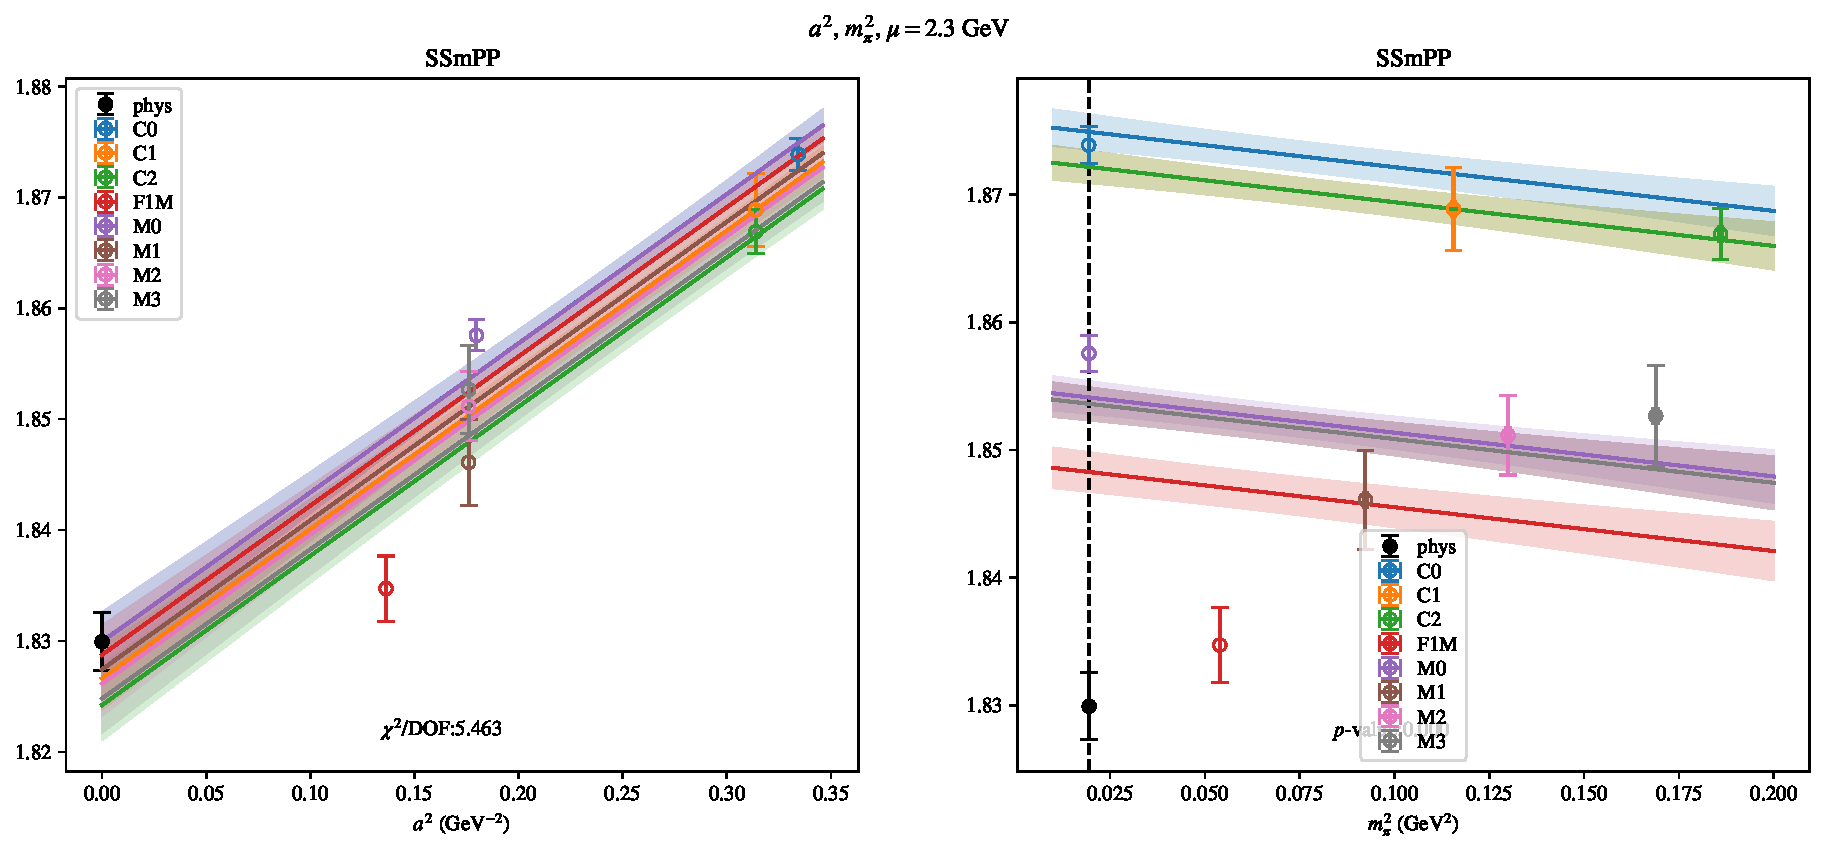
\includepdf[link, pages=-]{SSmPP/NPR/a2m2_23.pdf}
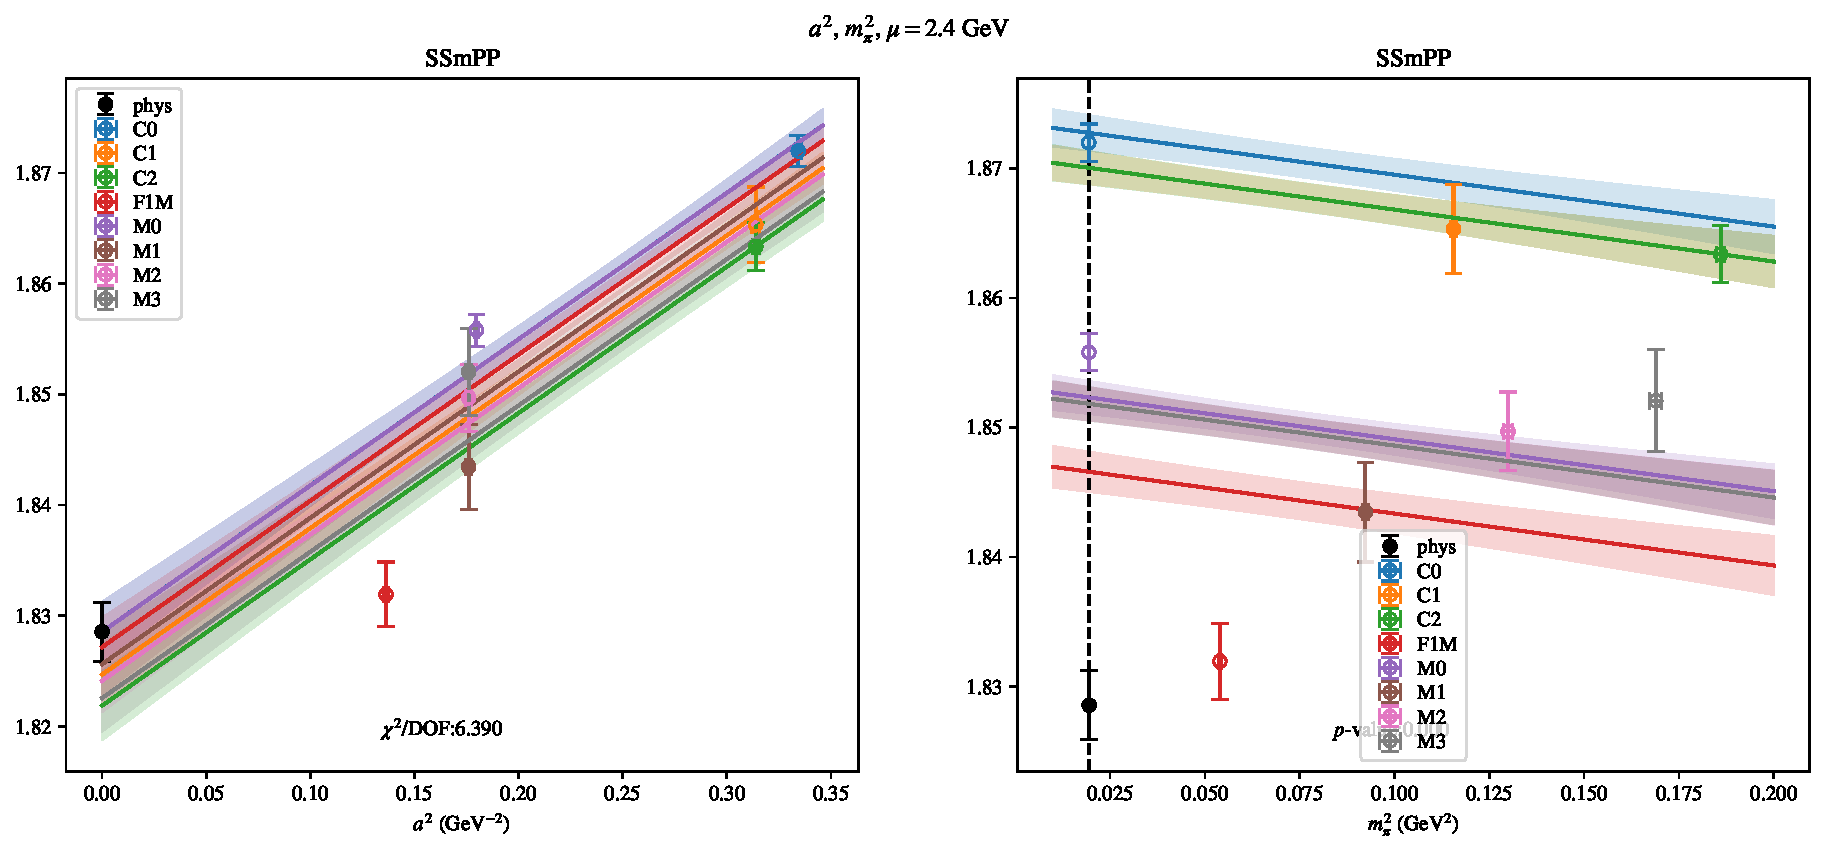
\includepdf[link, pages=-]{SSmPP/NPR/a2m2_24.pdf}
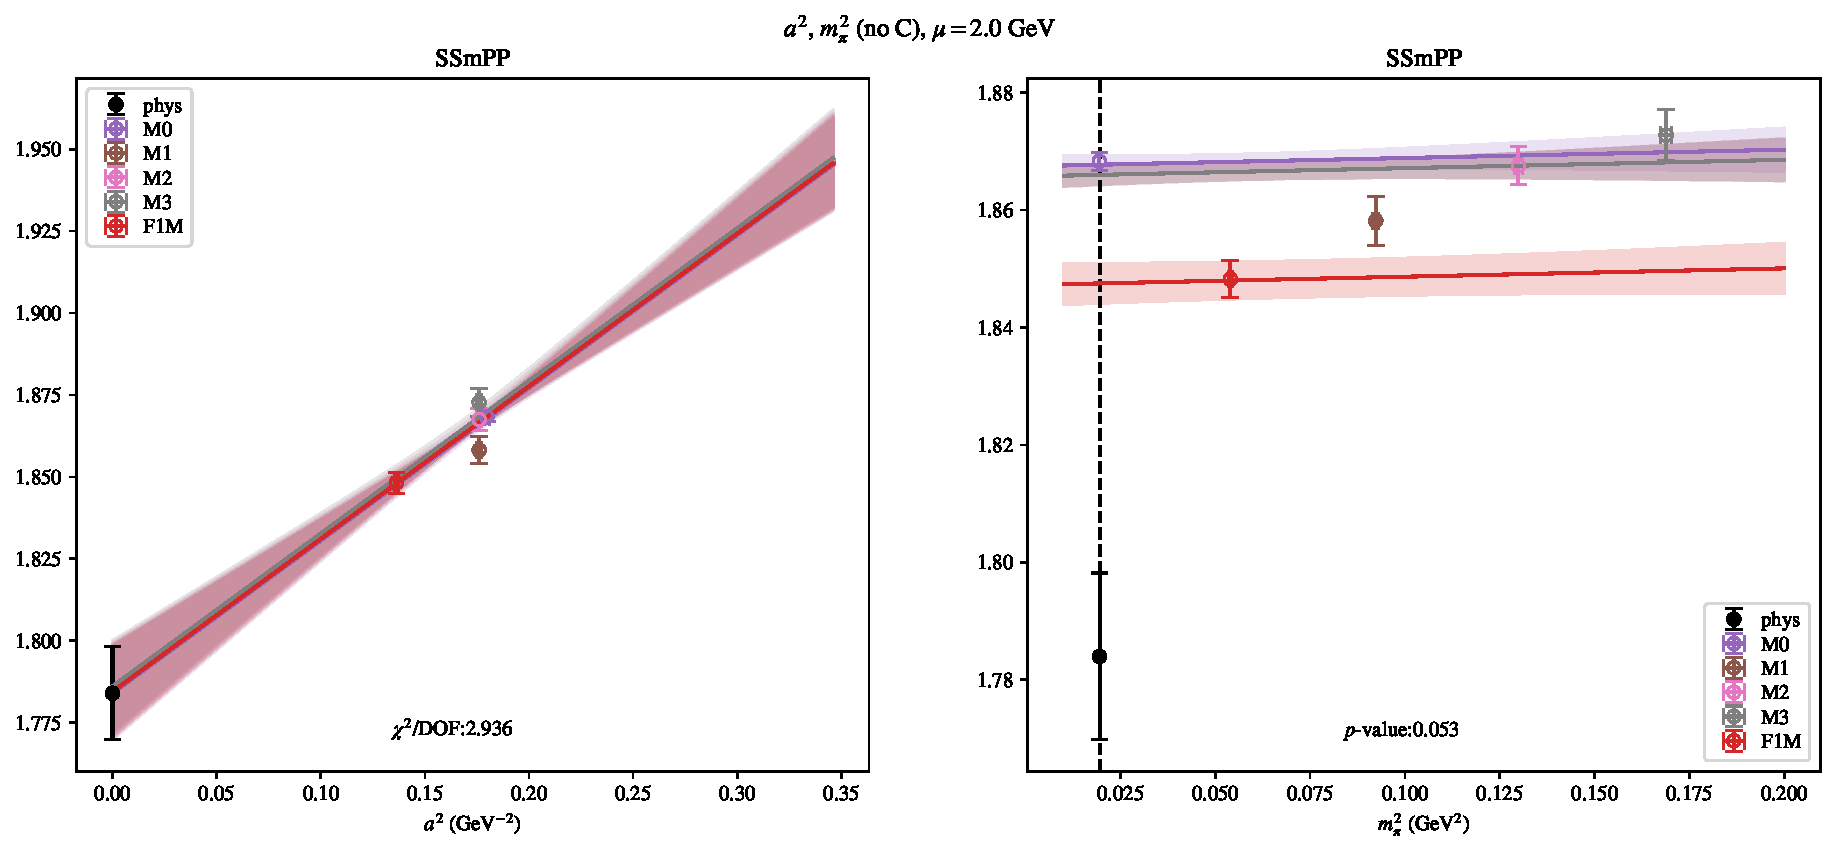
\includepdf[link, pages=-]{SSmPP/NPR/a2m2noC_20.pdf}
\includepdf[link, pages=-]{SSmPP/NPR/a2m2noC_22.pdf}
\includepdf[link, pages=-]{SSmPP/NPR/a2m2noC_23.pdf}
\includepdf[link, pages=-]{SSmPP/NPR/a2m2noC_24.pdf}
\includepdf[link, pages=-]{SSmPP/NPR/a2a4m2_20.pdf}
\includepdf[link, pages=-]{SSmPP/NPR/a2a4m2_22.pdf}
\includepdf[link, pages=-]{SSmPP/NPR/a2a4m2_23.pdf}
\includepdf[link, pages=-]{SSmPP/NPR/a2a4m2_24.pdf}
\includepdf[link, pages=-]{SSmPP/NPR/a2m2mcut_20.pdf}
\includepdf[link, pages=-]{SSmPP/NPR/a2m2mcut_22.pdf}
\includepdf[link, pages=-]{SSmPP/NPR/a2m2mcut_23.pdf}
\includepdf[link, pages=-]{SSmPP/NPR/a2m2mcut_24.pdf}
\includepdf[link, pages=-]{SSmPP/NPR/a2m2m4_20.pdf}
\includepdf[link, pages=-]{SSmPP/NPR/a2m2m4_22.pdf}
\includepdf[link, pages=-]{SSmPP/NPR/a2m2m4_23.pdf}
\includepdf[link, pages=-]{SSmPP/NPR/a2m2m4_24.pdf}
\clearpage
\section{$\mathcal{B}_4$}
\begin{table}[h!]
\begin{center}
\begin{tabular}{|c|c|c|c|c|c|}
\hline
$\mu$ (GeV) & $a^2$, $m_\pi^2$& $a^2$, $m_\pi^2$ (no C)& $a^2$, $a^4$, $m_\pi^2$& $a^2$, $m_\pi^2$ (no M3, C2)& $a^2$, $m_\pi^2$, $m_\pi^4$\\
\hline
2.0& \hyperlink{SSpPP/NPR/a2m2_20.pdf.1}{\textbf{-0.925(17)}: 2.877 (0.013)} & \hyperlink{SSpPP/NPR/a2m2noC_20.pdf.1}{\textbf{-0.936(97)}: 2.265 (0.104)} & \hyperlink{SSpPP/NPR/a2a4m2_20.pdf.1}{\textbf{-0.92(16)}: 3.596 (0.006)} & \hyperlink{SSpPP/NPR/a2m2mcut_20.pdf.1}{\textbf{-0.925(18)}: 3.242 (0.021)} & \hyperlink{SSpPP/NPR/a2m2m4_20.pdf.1}{\textbf{-0.924(19)}: 2.634 (0.032)}\\
2.2& \hyperlink{SSpPP/NPR/a2m2_22.pdf.1}{\textbf{-0.905(17)}: 3.984 (0.001)} & \hyperlink{SSpPP/NPR/a2m2noC_22.pdf.1}{\textbf{-0.920(91)}: 1.869 (0.154)} & \hyperlink{SSpPP/NPR/a2a4m2_22.pdf.1}{\textbf{-0.90(15)}: 4.98 (0.001)} & \hyperlink{SSpPP/NPR/a2m2mcut_22.pdf.1}{\textbf{-0.906(18)}: 4.341 (0.005)} & \hyperlink{SSpPP/NPR/a2m2m4_22.pdf.1}{\textbf{-0.904(18)}: 4.211 (0.002)}\\
2.3& \hyperlink{SSpPP/NPR/a2m2_23.pdf.1}{\textbf{-0.897(17)}: 4.483 (0.0)} & \hyperlink{SSpPP/NPR/a2m2noC_23.pdf.1}{\textbf{-0.913(90)}: 2.157 (0.116)} & \hyperlink{SSpPP/NPR/a2a4m2_23.pdf.1}{\textbf{-0.90(15)}: 5.592 (0.0)} & \hyperlink{SSpPP/NPR/a2m2mcut_23.pdf.1}{\textbf{-0.897(18)}: 5.069 (0.002)} & \hyperlink{SSpPP/NPR/a2m2m4_23.pdf.1}{\textbf{-0.895(18)}: 4.659 (0.001)}\\
2.4& \hyperlink{SSpPP/NPR/a2m2_24.pdf.1}{\textbf{-0.889(16)}: 4.89 (0.0)} & \hyperlink{SSpPP/NPR/a2m2noC_24.pdf.1}{\textbf{-0.906(89)}: 2.33 (0.097)} & \hyperlink{SSpPP/NPR/a2a4m2_24.pdf.1}{\textbf{-0.89(15)}: 6.105 (0.0)} & \hyperlink{SSpPP/NPR/a2m2mcut_24.pdf.1}{\textbf{-0.889(18)}: 5.647 (0.001)} & \hyperlink{SSpPP/NPR/a2m2m4_24.pdf.1}{\textbf{-0.887(18)}: 5.184 (0.0)}\\
\hline
\end{tabular}
\caption{Physical point value from chiral and continuum extrapolation at renormalisation scale $\mu$. Entries are \textbf{value(error)}: $\chi^2/\text{DOF}$ ($p$-value).}
\end{center}
\end{table}
\begin{table}[h!]
\begin{center}
\begin{tabular}{|c c|c|c|c|c|c|}
\hline
$\mu$ (GeV) &  & $a^2$, $m_\pi^2$& $a^2$, $m_\pi^2$ (no C)& $a^2$, $a^4$, $m_\pi^2$& $a^2$, $m_\pi^2$ (no M3, C2)& $a^2$, $m_\pi^2$, $m_\pi^4$\\
\hline
\multirow{2}{0.5in}{2.0} & $\alpha$ & 0.3758(79)& 0.307(63)& 0.37(16)& 0.3756(84)& 0.3817(85)\\
 & $\beta$ & 0.00665(16)& 0.00612(27)& 0.00665(17)& 0.00702(26)& 0.00832(80)\\
\hline
\multirow{2}{0.5in}{2.2} & $\alpha$ & 0.4232(81)& 0.329(60)& 0.41(16)& 0.4197(85)& 0.4282(86)\\
 & $\beta$ & 0.00705(15)& 0.00634(24)& 0.00704(17)& 0.00735(25)& 0.00847(74)\\
\hline
\multirow{2}{0.5in}{2.3} & $\alpha$ & 0.4449(81)& 0.337(60)& 0.41(16)& 0.4417(86)& 0.4506(88)\\
 & $\beta$ & 0.00714(15)& 0.00642(22)& 0.00712(17)& 0.00746(25)& 0.00868(75)\\
\hline
\multirow{2}{0.5in}{2.4} & $\alpha$ & 0.4640(81)& 0.354(60)& 0.43(16)& 0.4604(87)& 0.4698(88)\\
 & $\beta$ & 0.00723(15)& 0.00650(22)& 0.00722(17)& 0.00753(25)& 0.00874(75)\\
\hline
\end{tabular}
\caption{Fit values of coefficients in $Q = Q_{phys} + \mathbf{\alpha} a^2 + \mathbf{\beta}\left(\frac{m_\pi^2}{f_\pi^2}-\frac{m_{\pi,PDG}^2}{f_\pi^2}\right) + \ldots$.}
\end{center}
\end{table}
\includepdf[link, pages=-]{SSpPP/NPR/a2m2_20.pdf}
\includepdf[link, pages=-]{SSpPP/NPR/a2m2_22.pdf}
\includepdf[link, pages=-]{SSpPP/NPR/a2m2_23.pdf}
\includepdf[link, pages=-]{SSpPP/NPR/a2m2_24.pdf}
\includepdf[link, pages=-]{SSpPP/NPR/a2m2noC_20.pdf}
\includepdf[link, pages=-]{SSpPP/NPR/a2m2noC_22.pdf}
\includepdf[link, pages=-]{SSpPP/NPR/a2m2noC_23.pdf}
\includepdf[link, pages=-]{SSpPP/NPR/a2m2noC_24.pdf}
\includepdf[link, pages=-]{SSpPP/NPR/a2a4m2_20.pdf}
\includepdf[link, pages=-]{SSpPP/NPR/a2a4m2_22.pdf}
\includepdf[link, pages=-]{SSpPP/NPR/a2a4m2_23.pdf}
\includepdf[link, pages=-]{SSpPP/NPR/a2a4m2_24.pdf}
\includepdf[link, pages=-]{SSpPP/NPR/a2m2mcut_20.pdf}
\includepdf[link, pages=-]{SSpPP/NPR/a2m2mcut_22.pdf}
\includepdf[link, pages=-]{SSpPP/NPR/a2m2mcut_23.pdf}
\includepdf[link, pages=-]{SSpPP/NPR/a2m2mcut_24.pdf}
\includepdf[link, pages=-]{SSpPP/NPR/a2m2m4_20.pdf}
\includepdf[link, pages=-]{SSpPP/NPR/a2m2m4_22.pdf}
\includepdf[link, pages=-]{SSpPP/NPR/a2m2m4_23.pdf}
\includepdf[link, pages=-]{SSpPP/NPR/a2m2m4_24.pdf}
\clearpage
\section{$\mathcal{B}_5$}
\begin{table}[h!]
\begin{center}
\begin{tabular}{|c|c|c|c|c|c|}
\hline
$\mu$ (GeV) & $a^2$, $m_\pi^2$& $a^2$, $m_\pi^2$ (no C)& $a^2$, $a^4$, $m_\pi^2$& $a^2$, $m_\pi^2$ (no M3, C2)& $a^2$, $m_\pi^2$, $m_\pi^4$\\
\hline
2.0& \hyperlink{TT/NPR/a2m2_20.pdf.1}{\textbf{-0.3625(68)}: 0.593 (0.706)} & \hyperlink{TT/NPR/a2m2noC_20.pdf.1}{\textbf{-0.364(44)}: 0.122 (0.885)} & \hyperlink{TT/NPR/a2a4m2_20.pdf.1}{\textbf{-0.361(71)}: 0.728 (0.573)} & \hyperlink{TT/NPR/a2m2mcut_20.pdf.1}{\textbf{-0.3626(71)}: 0.683 (0.563)} & \hyperlink{TT/NPR/a2m2m4_20.pdf.1}{\textbf{-0.3624(70)}: 0.632 (0.64)}\\
2.2& \hyperlink{TT/NPR/a2m2_22.pdf.1}{\textbf{-0.3597(66)}: 0.949 (0.448)} & \hyperlink{TT/NPR/a2m2noC_22.pdf.1}{\textbf{-0.362(40)}: 0.264 (0.768)} & \hyperlink{TT/NPR/a2a4m2_22.pdf.1}{\textbf{-0.358(64)}: 1.181 (0.317)} & \hyperlink{TT/NPR/a2m2mcut_22.pdf.1}{\textbf{-0.3599(70)}: 1.358 (0.254)} & \hyperlink{TT/NPR/a2m2m4_22.pdf.1}{\textbf{-0.3597(69)}: 1.181 (0.317)}\\
2.3& \hyperlink{TT/NPR/a2m2_23.pdf.1}{\textbf{-0.3587(65)}: 1.006 (0.412)} & \hyperlink{TT/NPR/a2m2noC_23.pdf.1}{\textbf{-0.361(39)}: 0.349 (0.705)} & \hyperlink{TT/NPR/a2a4m2_23.pdf.1}{\textbf{-0.357(63)}: 1.253 (0.286)} & \hyperlink{TT/NPR/a2m2mcut_23.pdf.1}{\textbf{-0.3588(69)}: 1.524 (0.206)} & \hyperlink{TT/NPR/a2m2m4_23.pdf.1}{\textbf{-0.3586(69)}: 1.167 (0.323)}\\
2.4& \hyperlink{TT/NPR/a2m2_24.pdf.1}{\textbf{-0.3578(64)}: 0.939 (0.454)} & \hyperlink{TT/NPR/a2m2noC_24.pdf.1}{\textbf{-0.360(38)}: 0.466 (0.627)} & \hyperlink{TT/NPR/a2a4m2_24.pdf.1}{\textbf{-0.357(62)}: 1.173 (0.32)} & \hyperlink{TT/NPR/a2m2mcut_24.pdf.1}{\textbf{-0.3578(69)}: 1.423 (0.234)} & \hyperlink{TT/NPR/a2m2m4_24.pdf.1}{\textbf{-0.3575(68)}: 0.989 (0.412)}\\
\hline
\end{tabular}
\caption{Physical point value from chiral and continuum extrapolation at renormalisation scale $\mu$. Entries are \textbf{value(error)}: $\chi^2/\text{DOF}$ ($p$-value).}
\end{center}
\end{table}
\begin{table}[h!]
\begin{center}
\begin{tabular}{|c c|c|c|c|c|c|}
\hline
$\mu$ (GeV) &  & $a^2$, $m_\pi^2$& $a^2$, $m_\pi^2$ (no C)& $a^2$, $a^4$, $m_\pi^2$& $a^2$, $m_\pi^2$ (no M3, C2)& $a^2$, $m_\pi^2$, $m_\pi^4$\\
\hline
\multirow{2}{0.5in}{2.0} & $\alpha$ & -0.038(72)& -0.07(68)& -0.002& -0.039(76)& -0.037(75)\\
 & $\beta$ & 0.00617(16)& 0.00584(31)& 0.00618(17)& 0.00630(25)& 0.00672(81)\\
\hline
\multirow{2}{0.5in}{2.2} & $\alpha$ & -0.079(71)& -0.12(62)& -0.057& -0.081(75)& -0.079(74)\\
 & $\beta$ & 0.00630(14)& 0.00590(26)& 0.00631(15)& 0.00627(22)& 0.00641(72)\\
\hline
\multirow{2}{0.5in}{2.3} & $\alpha$ & -0.103(70)& -0.14(61)& -0.084& -0.104(74)& -0.102(73)\\
 & $\beta$ & 0.00630(14)& 0.00597(24)& 0.00631(15)& 0.00636(22)& 0.00675(71)\\
\hline
\multirow{2}{0.5in}{2.4} & $\alpha$ & -0.128(69)& -0.16(60)& -0.1(15)& -0.128(73)& -0.126(72)\\
 & $\beta$ & 0.00627(14)& 0.00600(24)& 0.00627(15)& 0.00637(22)& 0.00690(70)\\
\hline
\end{tabular}
\caption{Fit values of coefficients in $Q = Q_{phys} + \mathbf{\alpha} a^2 + \mathbf{\beta}\left(\frac{m_\pi^2}{f_\pi^2}-\frac{m_{\pi,PDG}^2}{f_\pi^2}\right) + \ldots$.}
\end{center}
\end{table}
\includepdf[link, pages=-]{TT/NPR/a2m2_20.pdf}
\includepdf[link, pages=-]{TT/NPR/a2m2_22.pdf}
\includepdf[link, pages=-]{TT/NPR/a2m2_23.pdf}
\includepdf[link, pages=-]{TT/NPR/a2m2_24.pdf}
\includepdf[link, pages=-]{TT/NPR/a2m2noC_20.pdf}
\includepdf[link, pages=-]{TT/NPR/a2m2noC_22.pdf}
\includepdf[link, pages=-]{TT/NPR/a2m2noC_23.pdf}
\includepdf[link, pages=-]{TT/NPR/a2m2noC_24.pdf}
\includepdf[link, pages=-]{TT/NPR/a2a4m2_20.pdf}
\includepdf[link, pages=-]{TT/NPR/a2a4m2_22.pdf}
\includepdf[link, pages=-]{TT/NPR/a2a4m2_23.pdf}
\includepdf[link, pages=-]{TT/NPR/a2a4m2_24.pdf}
\includepdf[link, pages=-]{TT/NPR/a2m2mcut_20.pdf}
\includepdf[link, pages=-]{TT/NPR/a2m2mcut_22.pdf}
\includepdf[link, pages=-]{TT/NPR/a2m2mcut_23.pdf}
\includepdf[link, pages=-]{TT/NPR/a2m2mcut_24.pdf}
\includepdf[link, pages=-]{TT/NPR/a2m2m4_20.pdf}
\includepdf[link, pages=-]{TT/NPR/a2m2m4_22.pdf}
\includepdf[link, pages=-]{TT/NPR/a2m2m4_23.pdf}
\includepdf[link, pages=-]{TT/NPR/a2m2m4_24.pdf}
\clearpage
\end{document}